\chapter{Result and Evaluation of Simulations}\label{chap:results}
In this chapter, we present the results of the simulations conducted across different topologies. The network sizes selected for these simulations are powers of 2. For a comprehensive overview of all simulations performed, refer to table \ref{table:overviewsims}. Additionally, we have conducted simulations with network sizes that are powers of 10, which are documented in the \hyperref[chap:appendix]{Appendix}.
The results are visualized using \textit{log-log graphs}, where both axes are on a logarithmic scale. The x-axis represents the number of rounds, while the y-axis indicates the mean squared error (MSE). For clarity, we will refer to the Single-Proposal-Deal-Agreement-Based protocol as \textit{DAB} and the Push-Pull Sum protocol as \textit{PPS} throughout this section. Each subsection will highlight a winner based on the performance metrics observed in the simulations.

\section{Complete Graphs}
\textbf{The complete graph}: The complete graph as illustrated in \hyperref[fig:completegraphDemo]{figure} \ref{fig:completegraphDemo} is a graph where each pair of distinct nodes is connected by an edge. The complete graph contains of $n$ nodes and $\frac{n\times(n-1)}{2}$ edges. Every node has a degree of $n-1$, since each node is connected to every other node except to itself. Due to its structure, the complete graph is considered a dense graph, as it contains the maximum possible number of edges for a given set of nodes \cite{GraphTheorySchindelhaauer2021}.
\begin{figure}[H]
    \centering
    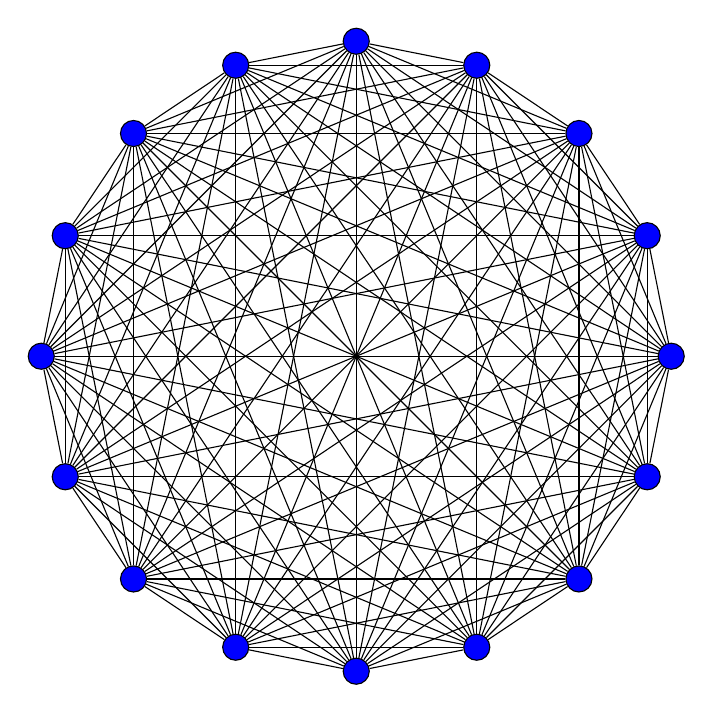
\begin{tikzpicture}
    \foreach \i in {1,...,16} {
      \node[draw, fill=blue, circle, minimum size=6pt] (v\i) at ({360/16 * (\i-1)}:4) {};
    }
    
    \foreach \i in {1,...,16} {
      \foreach \j in {1,...,16} {
        \ifnum\i<\j
          \draw (v\i) -- (v\j);
        \fi
      }
    }
    
  \end{tikzpicture}
    \caption{complete graph: network size 16}
    \label{fig:completegraphDemo}
\end{figure}
\subsection{Network Size 2\textsuperscript{4}}
\textbf{Figures}: \ref{fig:16CompleteGraph}\\
\textbf{Observations}: The plot in figure \ref{fig:16CompleteGraph} illustrates the performance of the DAB and PPS on a complete graph with a network size of 16 (resulting in 120 edges). In the beginning the mean squared error of the network balanced by the DAB algorithm does not decrease as fast as that of the PPS algorithm. However, in round 29, the DAB successfully reduces the MSE to 0, indicating a perfectly balanced network where all nodes have identical loads. This is the state we are aiming for by applying the load balancing algorithms.

Despite the initially steeper downward slope of the PPS graph, the DAB manages to balance the graph more quickly. The remaining simulation showed that in some cases the DAB protocol reduces the error of the network faster, however there are cases like in the \hyperref[chap:appendix]{Appendix} where the PPS performs better for small network sizes.

The PPS chooses its transfer partners by random. For the PPS each load transfer step involves a push and a pull operation. In smaller networks, PPS cannot fully exploit the high connectivity of the graph, limiting its effectiveness. A larger network size, means more edges, which results in more messages being sent trough the network, resulting in a good performance of decreasing the MSE \cite{nugroho2023PushPullSumDataAg}. For a small network size DAB performs well. In some cases, DAB is even able to balance the network completely, as can be seen in figure \ref{fig:16CompleteGraph}. As the network size increases, the PPS outperforms the DAB.\\
\begin{figure}[H]
    \centering
    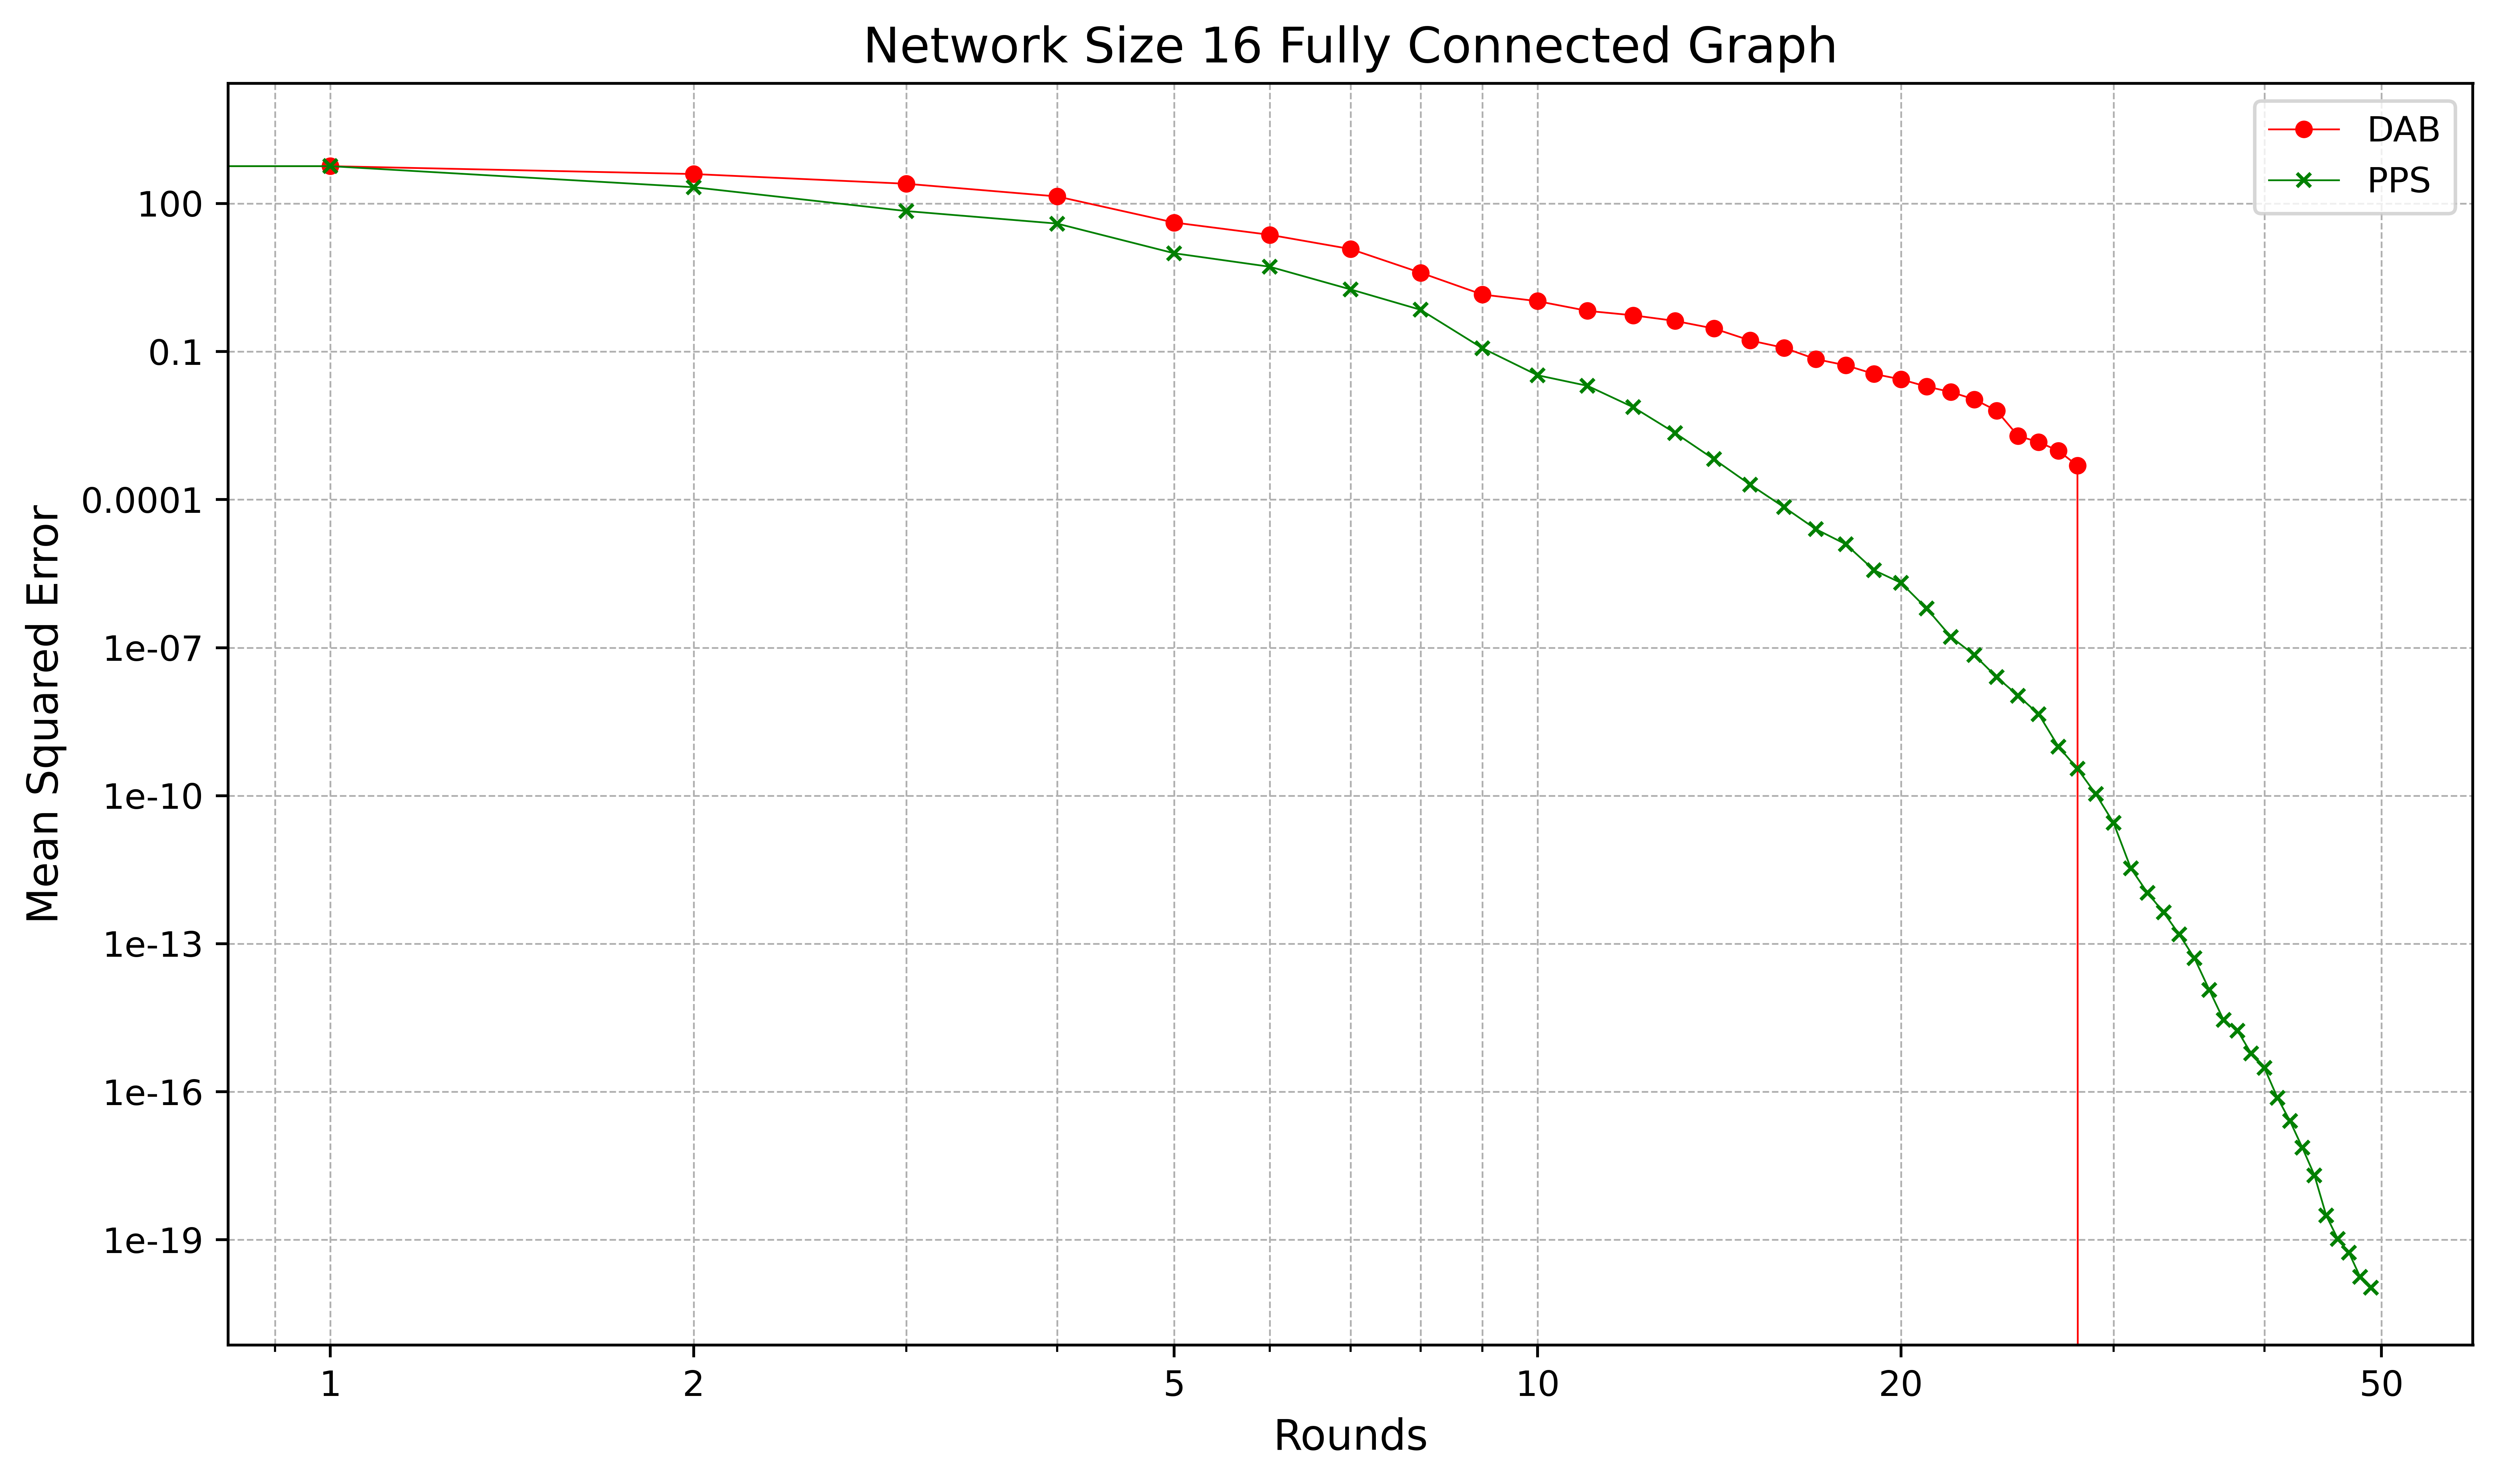
\includegraphics[scale=0.5]{figures/completeGraphSimulations/DAB_vs_PPS_FCG_r50_n16.png}
    \caption{Fully connected graph: network size $2^{4}$ nodes}
    \label{fig:16CompleteGraph}
\end{figure}

\subsection{Network Sizes 2\textsuperscript{8}, 2\textsuperscript{12}, 2\textsuperscript{14}}
\textbf{Figures}: \ref{fig:256CompleteGraph}, \ref{fig:4096CompleteGraph}, \ref{fig:16384CompleteGraph}\\
\textbf{Observations}: For larger network sizes PPS outperforms DAB. The plots of figures \ref{fig:256CompleteGraph}, \ref{fig:4096CompleteGraph} and \ref{fig:16384CompleteGraph} indicate this very clearly. The plots show that DAB maintains a consistent MSE of the network of around 1.000 across all rounds, indicating that it does not improve significantly over time. PPS, on the other hand reaches a significant decrease in MSE as the number of rounds increases, indicating that PPS improves the state of the network a lot better than DAB with more rounds and achieves a much lower error, reaching down to less than $1e-14$.\\
The slope of the PPS graph becomes steeper as rounds increase, indicating rapid convergence and an exponential improvement in performance with each additional round.\\
\begin{figure}[H]
    \centering
    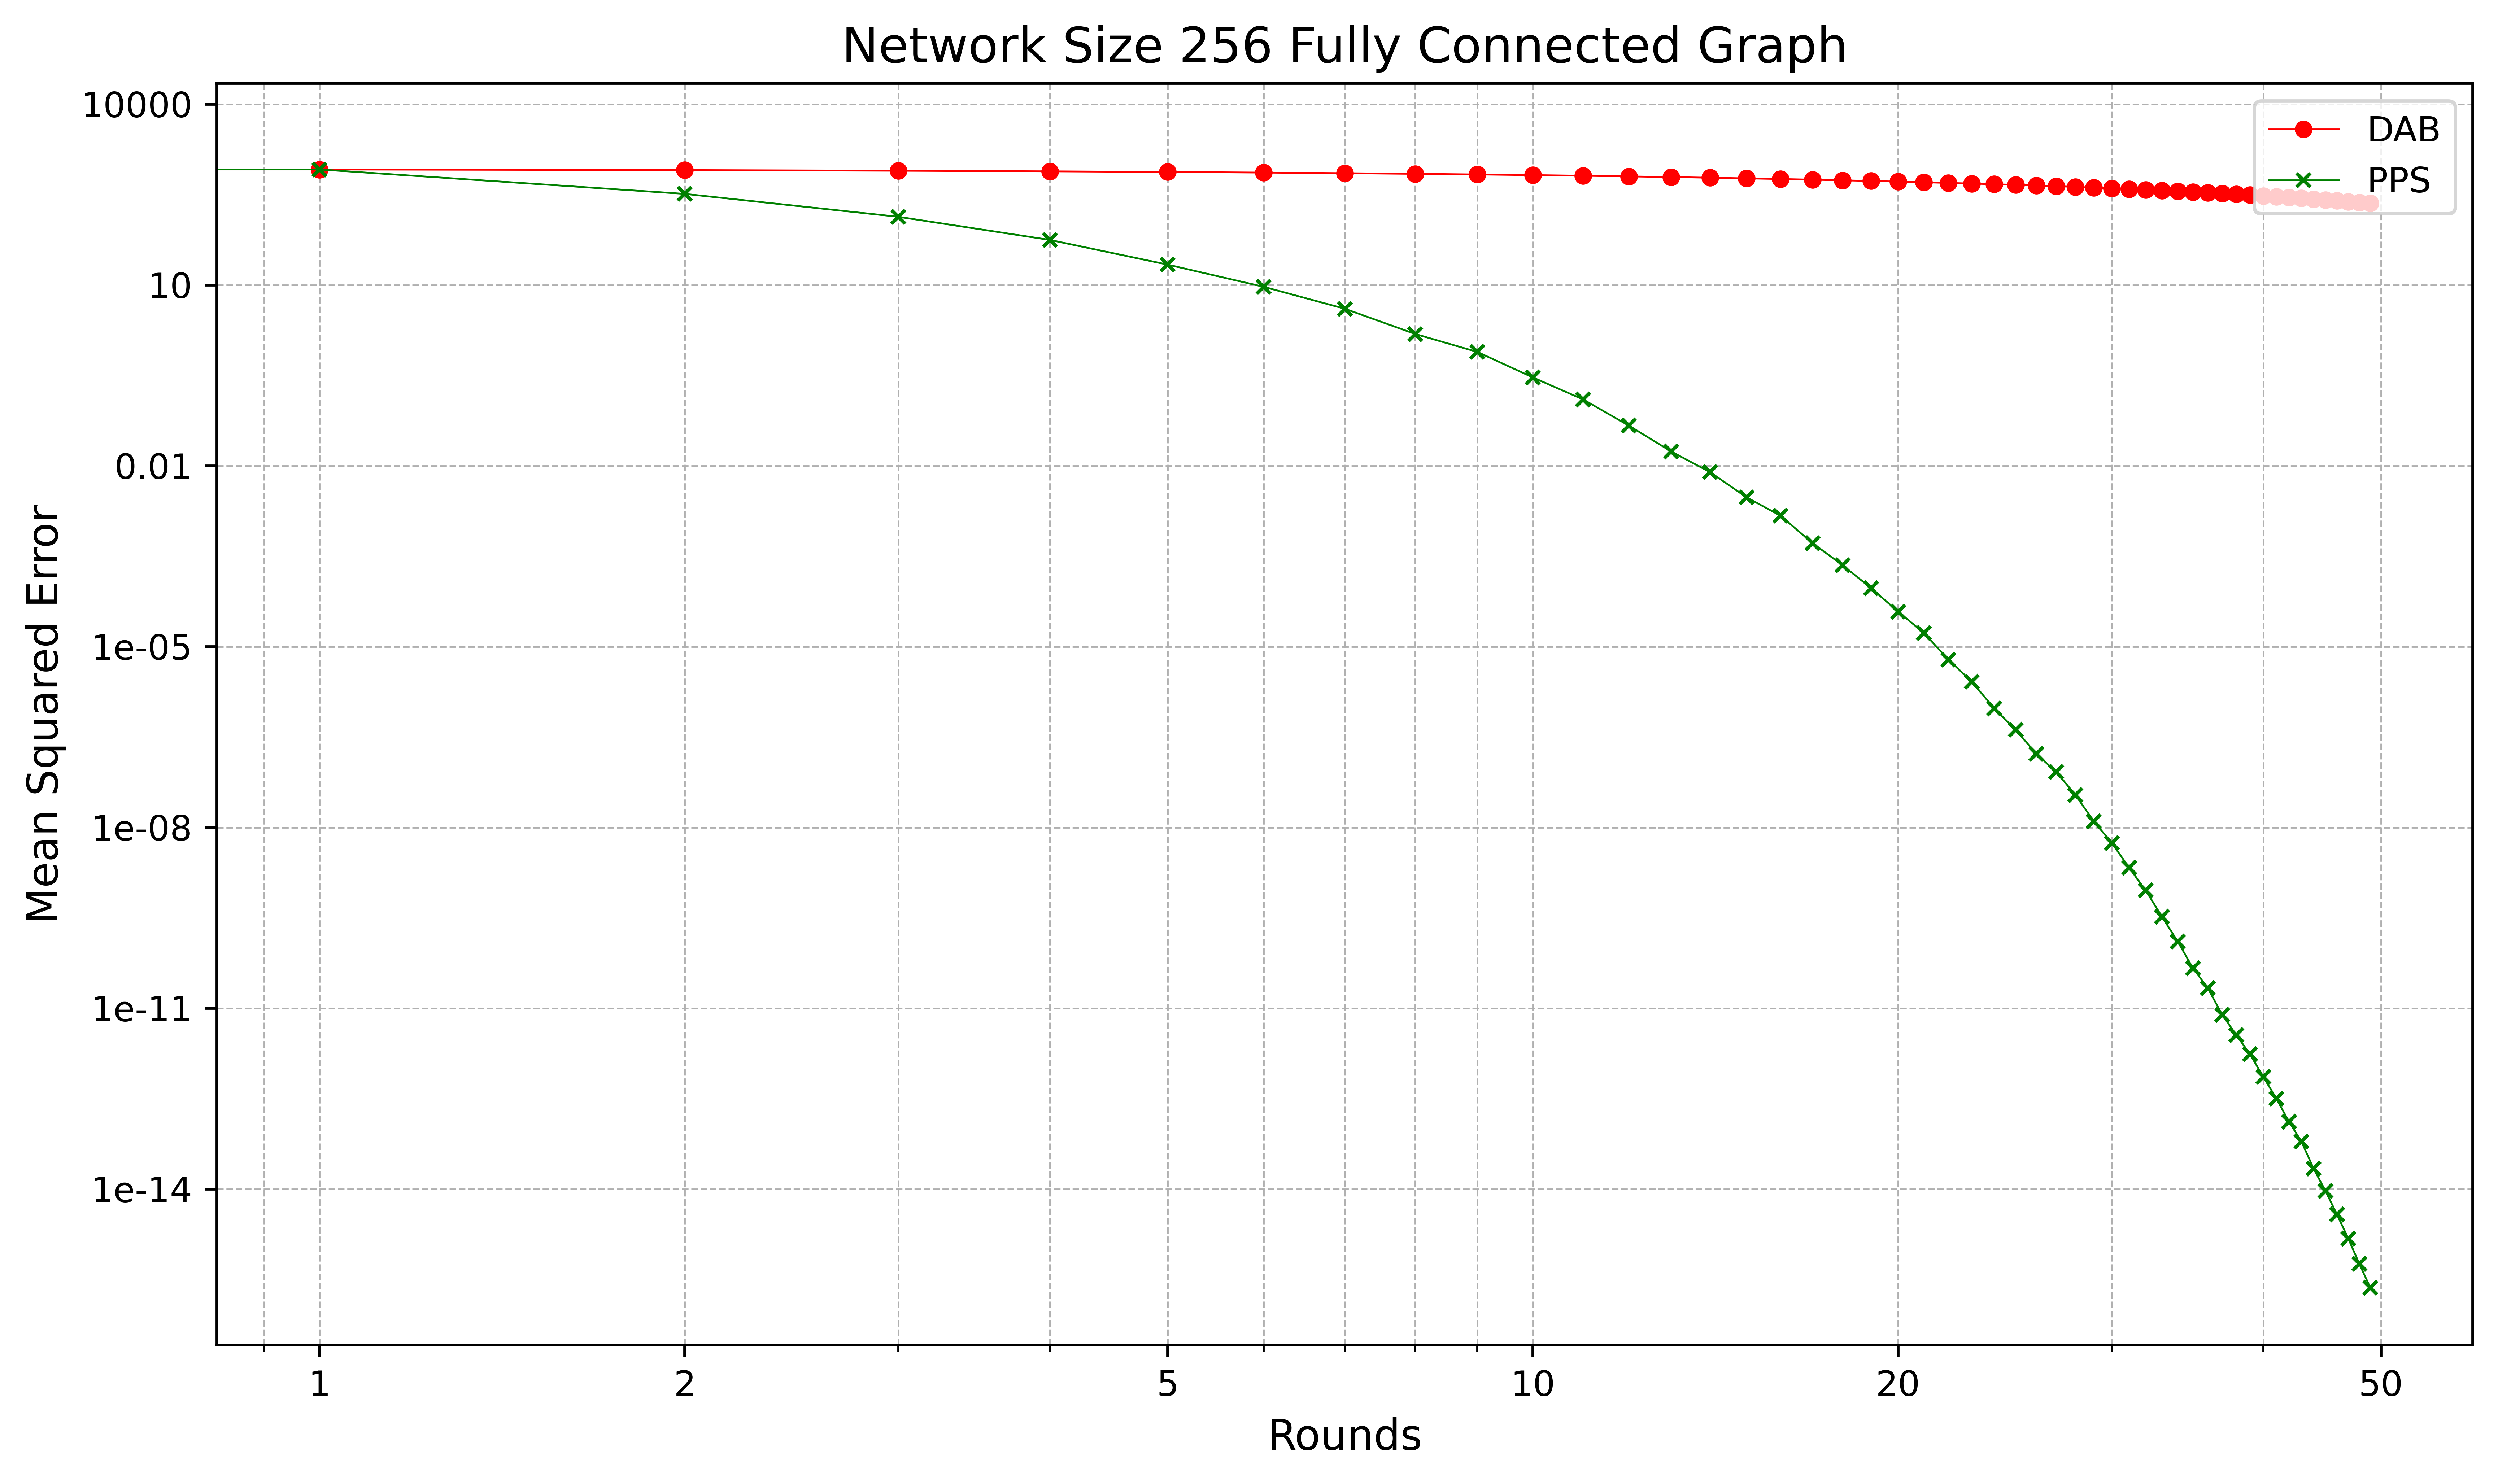
\includegraphics[scale=0.5]{figures/completeGraphSimulations/DAB_vs_PPS_FCG_r50_n256.png}
    \caption{Fully connected graph: network size $2^{8}$ nodes}
    \label{fig:256CompleteGraph}
\end{figure}

\begin{figure}[H]
    \centering
    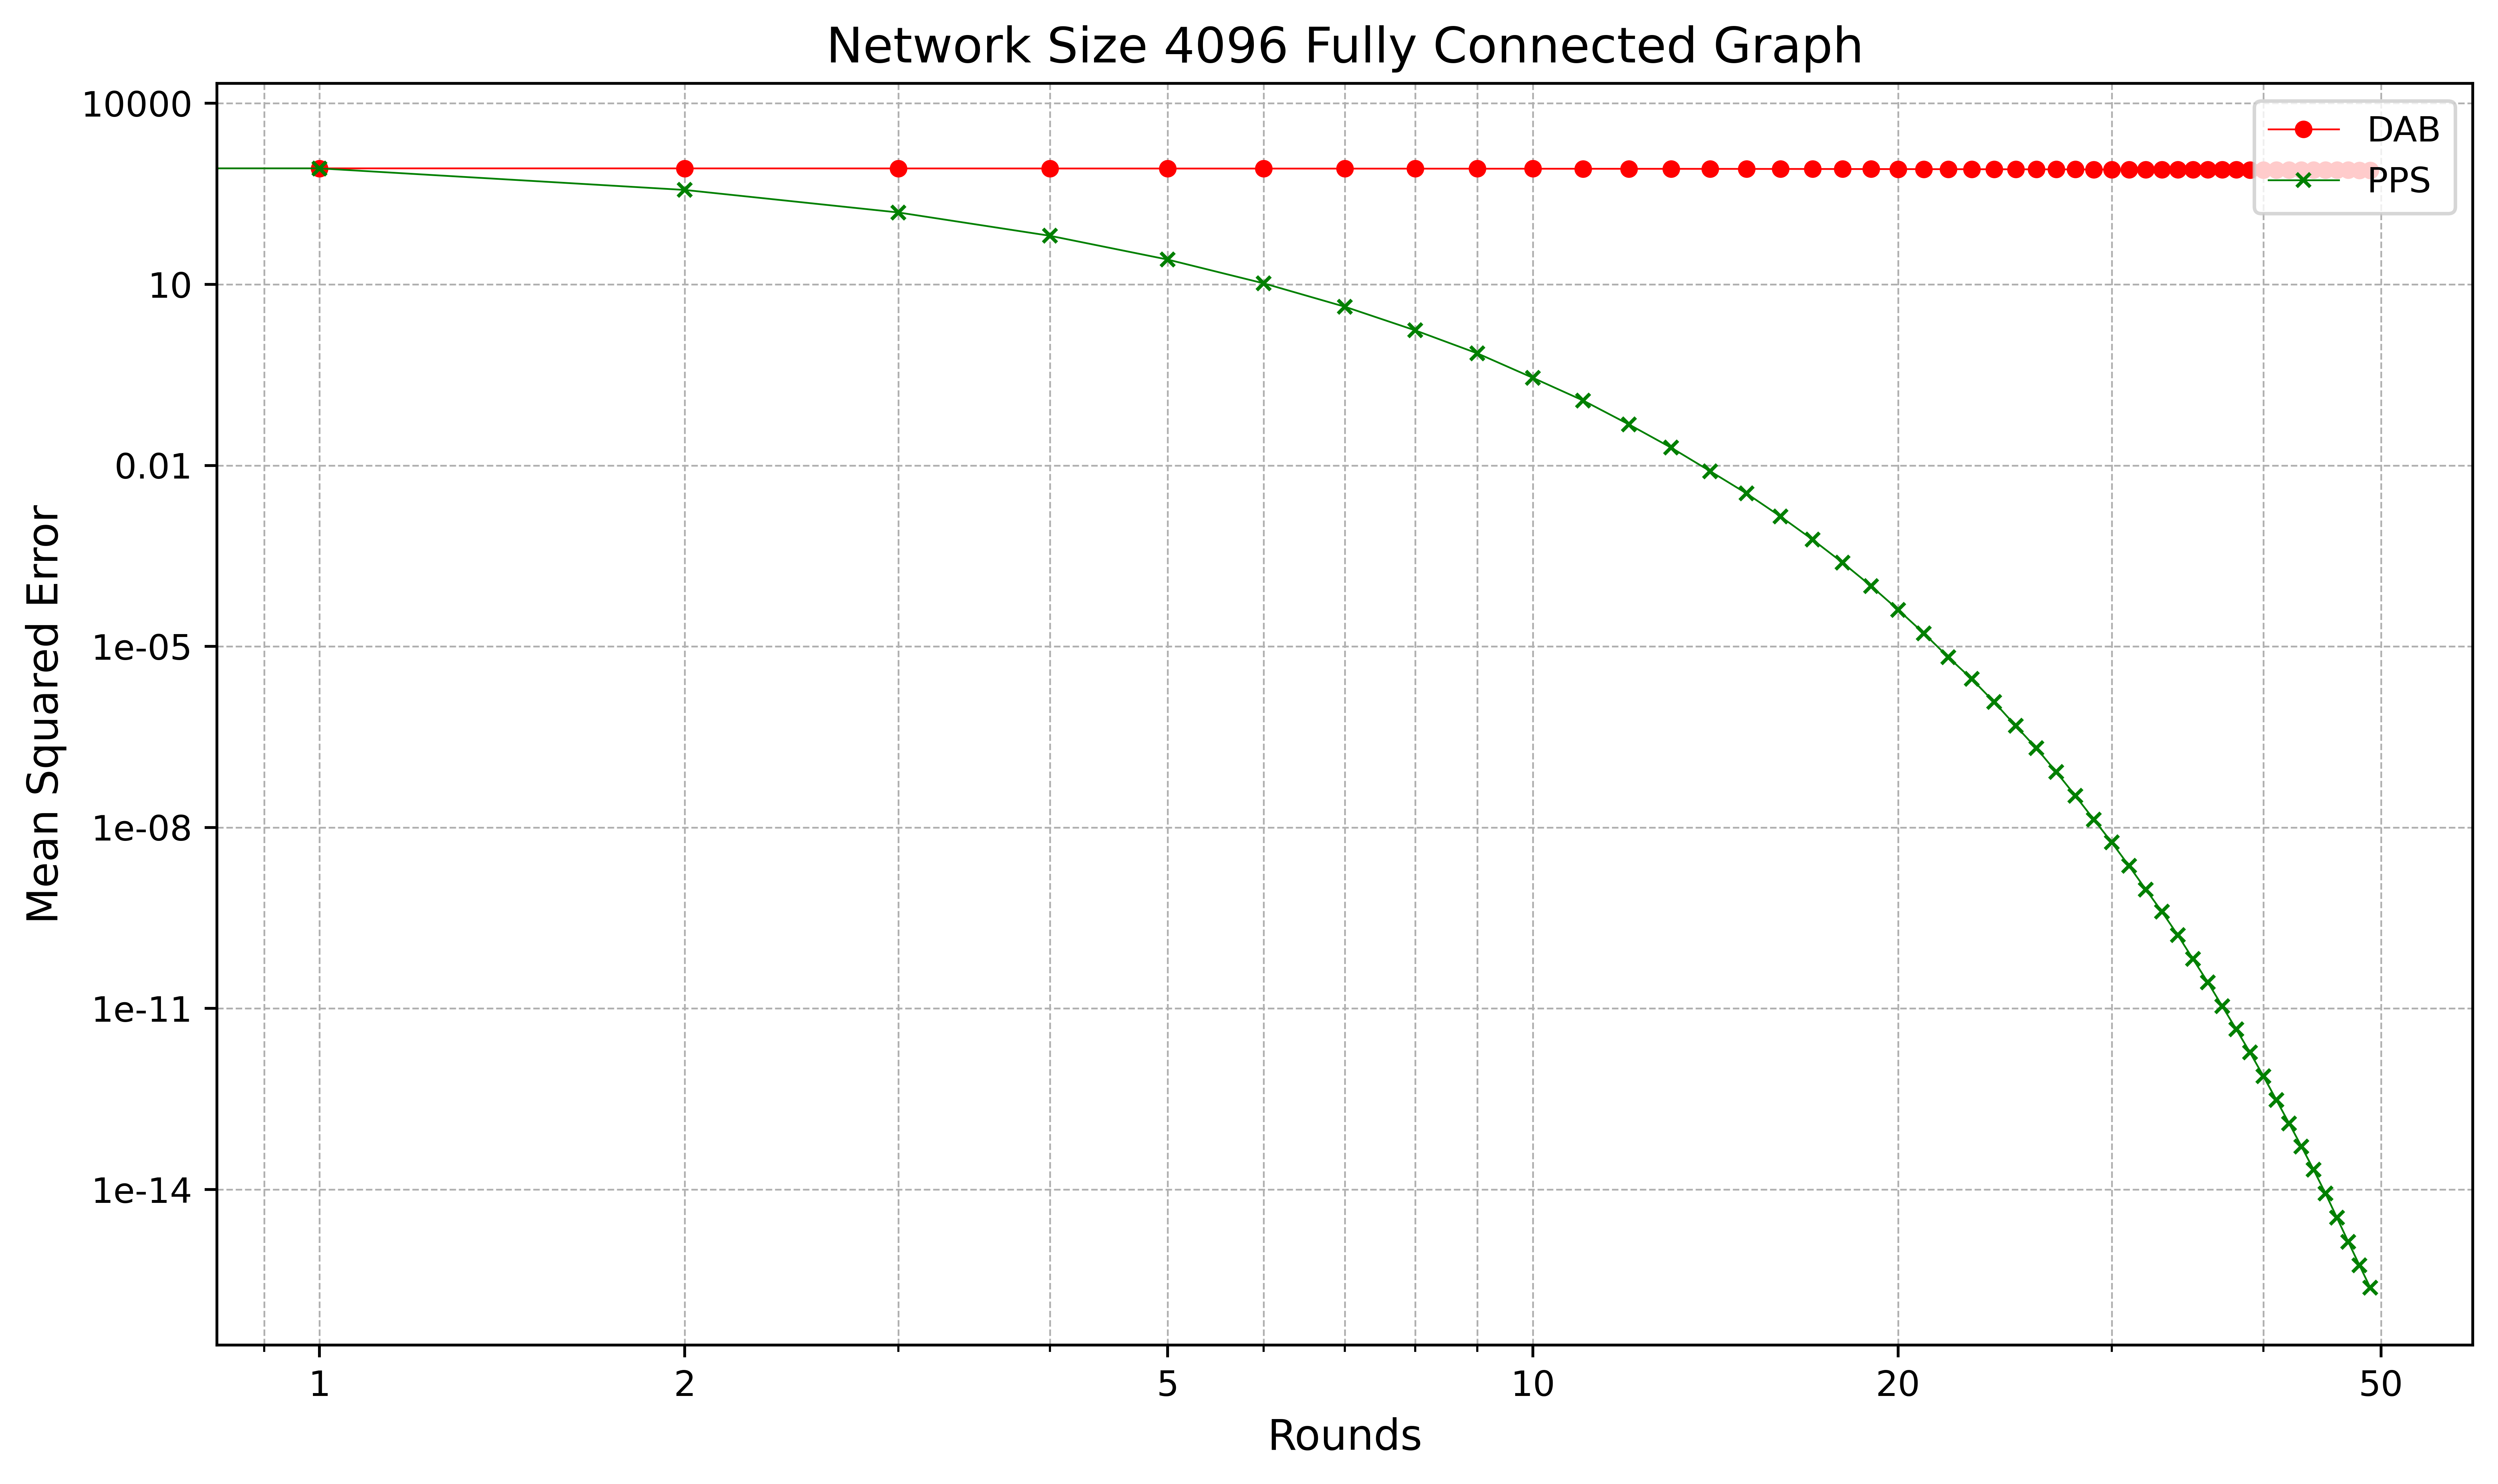
\includegraphics[scale=0.5]{figures/completeGraphSimulations/DAB_vs_PPS_FCG_r50_n4096.png}
    \caption{Fully connected graph: network size $2^{12}$ nodes}
    \label{fig:4096CompleteGraph}
\end{figure}
\begin{figure}[H]
    \centering
    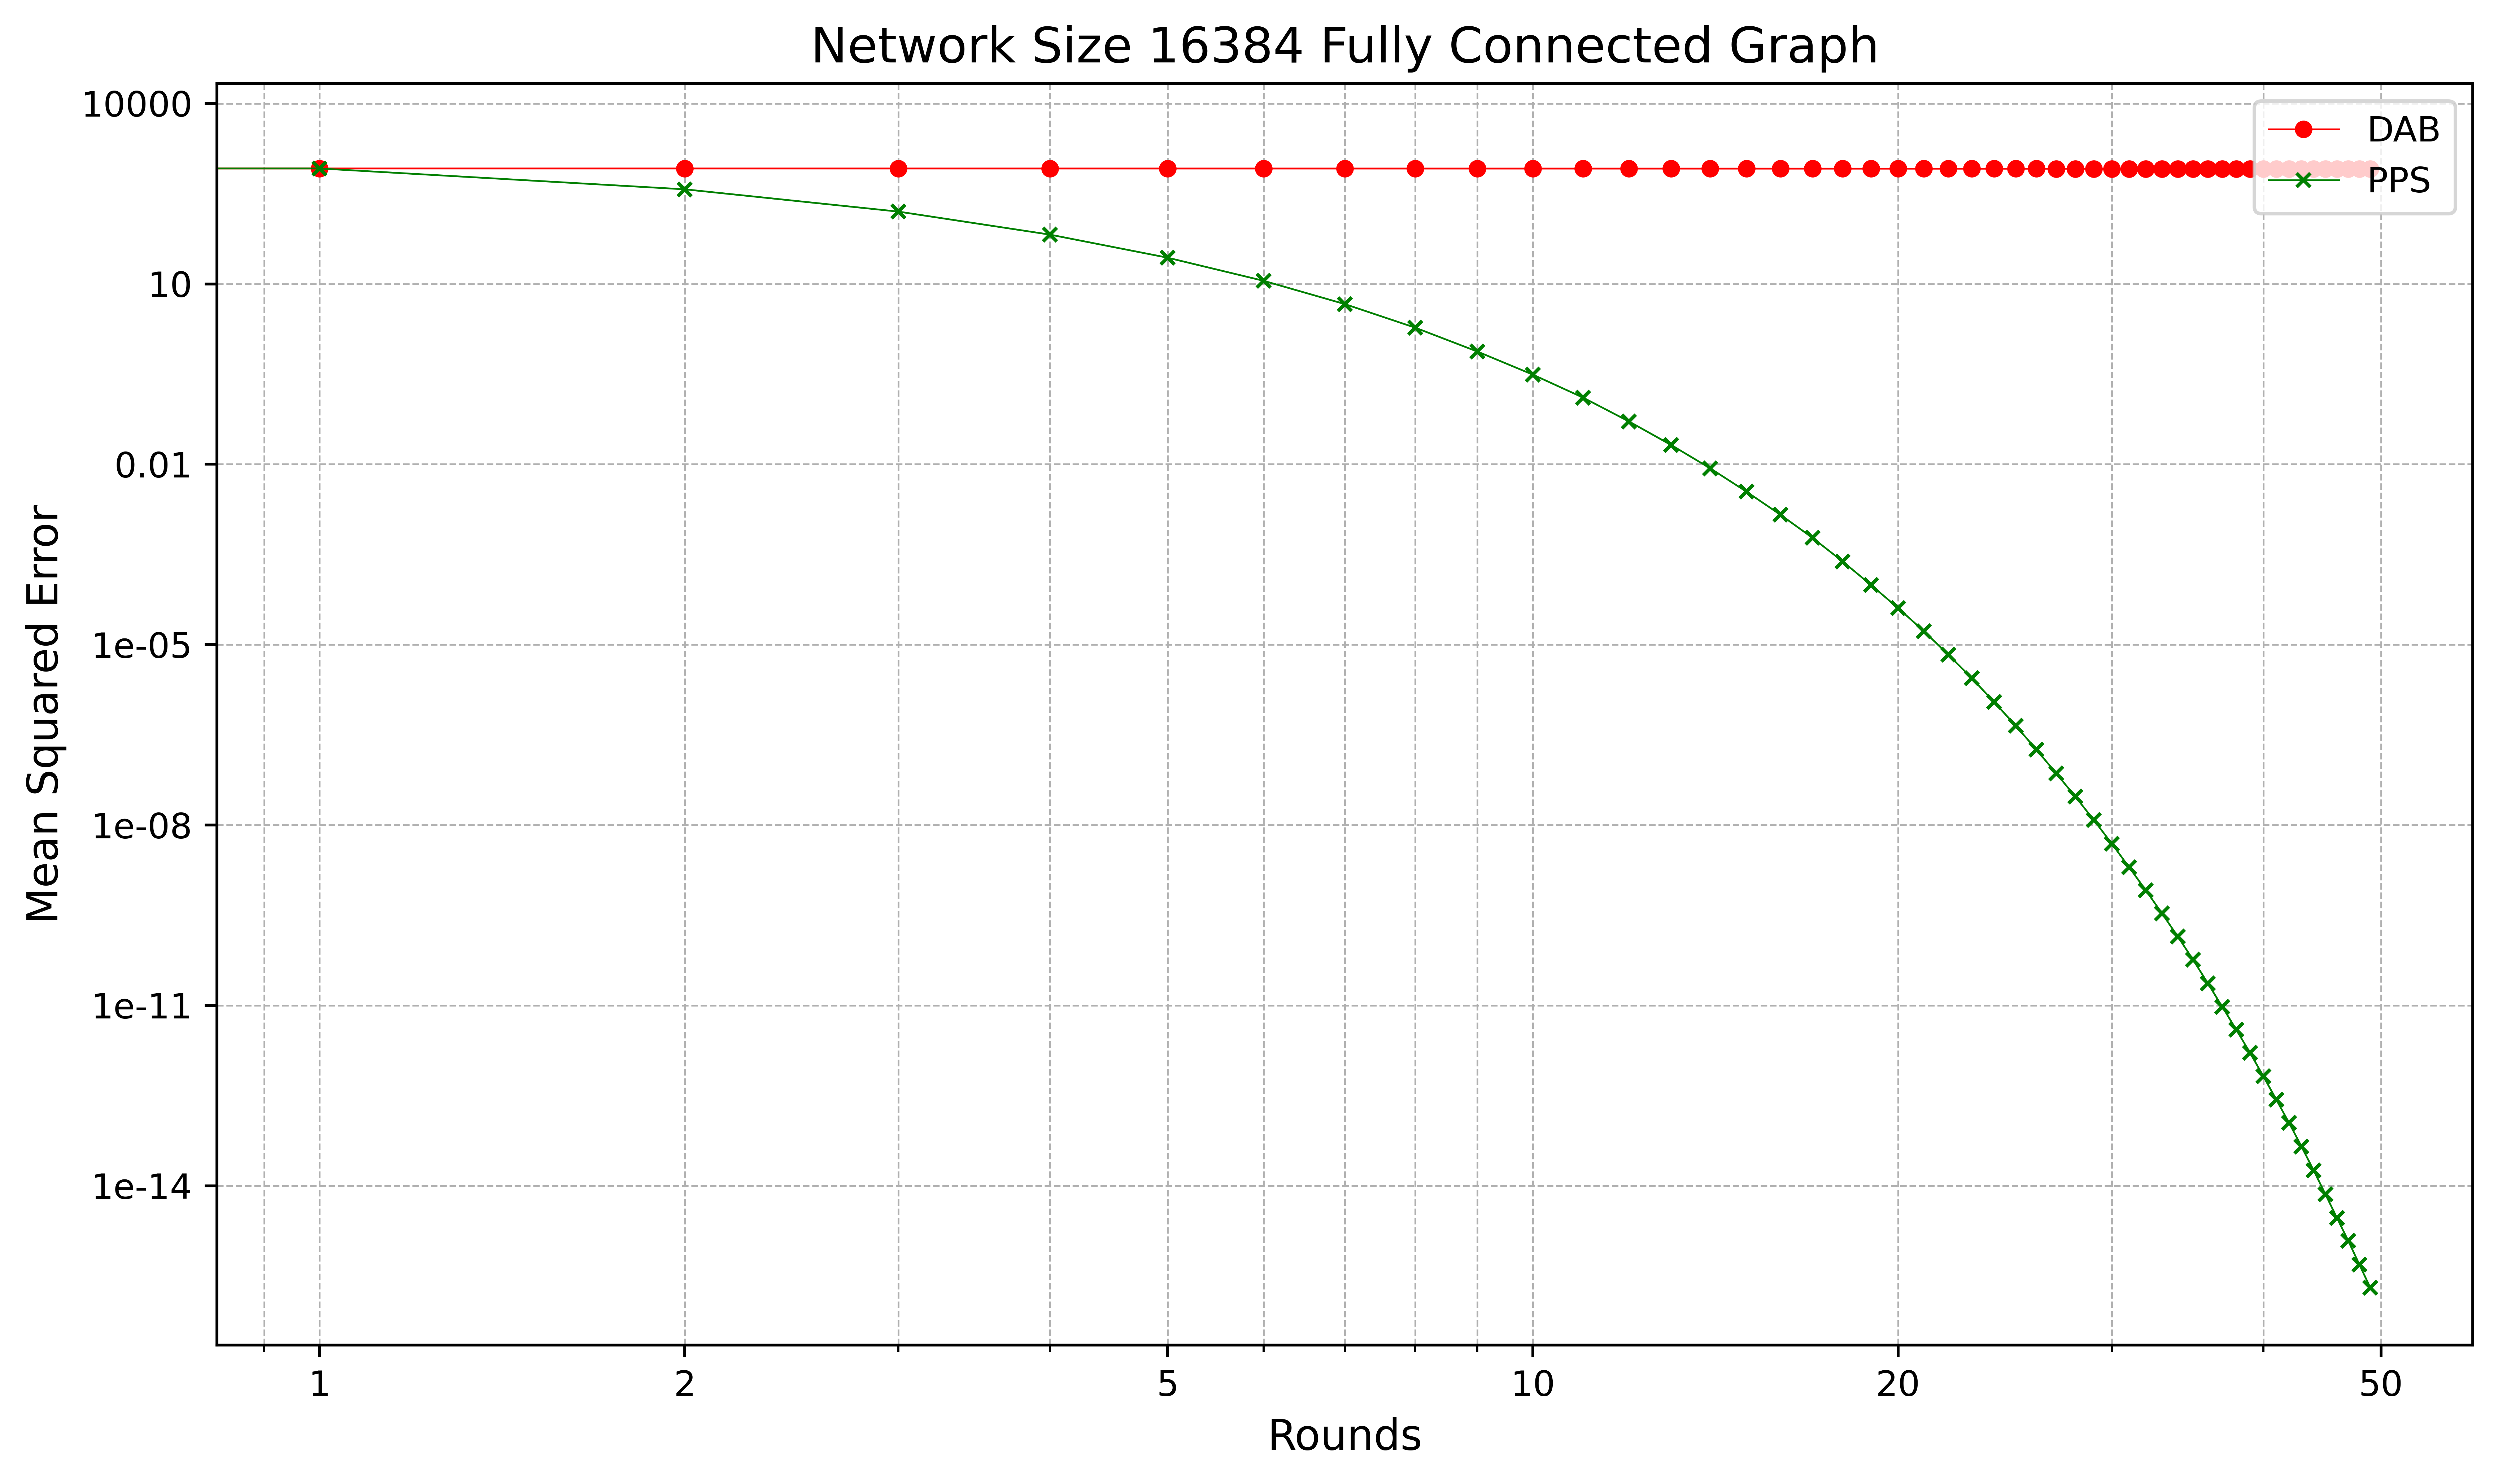
\includegraphics[scale=0.5]{figures/completeGraphSimulations/DAB_vs_PPS_FCG_r50_n16384.png}
    \caption{Fully connected graph: network size $2^{14}$ nodes}
    \label{fig:16384CompleteGraph}
\end{figure}


\section{Star Graph}
\textbf{The star graph}: A star graph as depicted in \hyperref[fig:stargraphDemo]{figure} \ref{fig:stargraphDemo} is a complete bipartite graph \cite{west2001introduction}. A graph is classified as bipartite graph, if the set of graph edges is the union of two disjoint independent sets \cite{GraphTheorySchindelhaauer2021}. In a star graph, the central node belongs to one of these sets, while all remaining outer nodes belong to the other set.

A star graph with $n$ nodes has $n-1$ edges. In this structure, every outer node has a degree of 1, meaning it is connected only to the central node. The central node has a degree of $n-1$. The diameter of a star graph is 2.
\begin{figure}[H]
    \centering
    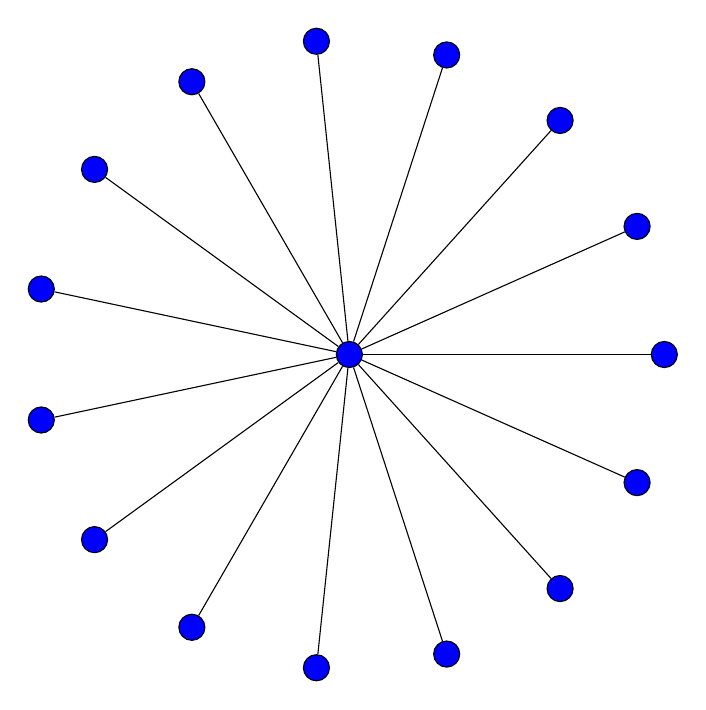
\begin{tikzpicture}
    \node[draw, fill=blue, circle] (center) at (0, 0) {};
    \foreach \i in {1,...,15} {
            \node[draw, fill=blue, circle] (n\i) at ({360/15 * (\i-1)}:4) {};
            \draw (center) -- (n\i);
        }
\end{tikzpicture}
    \caption{Star graph: network size 16}
    \label{fig:stargraphDemo}
\end{figure}
\subsection{Network Sizes 2\textsuperscript{4}, 2\textsuperscript{8}, 2\textsuperscript{12}, 2\textsuperscript{14}}
\textbf{Figures}: \ref{fig:16StarGraph}, \ref{fig:256StarGraph}, \ref{fig:4096StarGraph}, \ref{fig:16384StarGraph}\\
\textbf{Observations}: The PPS algorithm outperforms the DAB in terms of error reduction in every network size we have simulated. For smaller network sizes, the network balanced by DAB shows some reduction in mean squared error, however "only" reduces the MSE to around 0.001 at the end. The network balanced with the PPS has reached an MSE of $1e-23$ at the end and is therefore far more balanced.

For larger network sizes, the network balanced by the DAB results in a stagnating MSE curve. A look at the simulation outputs shows: For the network sizes $2^{8}$, $2^{12}$ and $2^{14}$, the MSE after 50 rounds for the DAB balanced network is located around 100. Meanwhile, the PPS balanced network achieves an MSE of less than $1e-20$.

This is due to the characteristic structure of the star graph. Each outer node is only connected to the center node. For all the outer nodes this means, that the only possible trading partner is the central node. Consequently, the DAB will, when searching for the minimum node, only be able to propose to the central node. If the central node's load is already higher than that of the outer nodes, load transfers are minimal or nonexistent, leading to a slow reduction in network error. The PPS, on the other hand, performs very well in this structure. Each outer node selects the center node as a trading partner. This means that every node is involved in a load transfer in each round. Each push action of the outer node is followed by a pull action of the center node. What is now observable, however, is that the central node becomes heavily stressed with load transfers, which could lead to failures due to overloading. This node fulfils a large part of the balancing procedure. It is notable that the sum and the weight value of the center node is larger than the ones of the outer nodes. If a node is involved in every load transfer, this results in a very one-sided load on a node. For the DAB in the star graph scenario there is also a one-sided loading of a node, however with less load transfers per round.

Another observation that emerges from the plot is that the PPS protocols graph has a spike in the last few rounds of the simulations for several network sizes. In rounds 47-50, there is a short-term increase in the error for the three network sizes $2^{8}$, $2^{12}$ and $2^{14}$. Such behaviour is not observed for the DAB protocol.

As the MSE decreases to extremely small values for the PPS graph (in the range of $1e-17$ to $1e-20$, as shown in the plot), the precision of the representation may begin to deteriorate. When numbers become very small, precision errors or underflows can occur, which lead to spikes in the computed values. This may be an explanation for the spikes occuring in the graphs and may not be a true reflection of the PPS performance (for the last few rounds).\\
\begin{figure}[H]
    \centering
    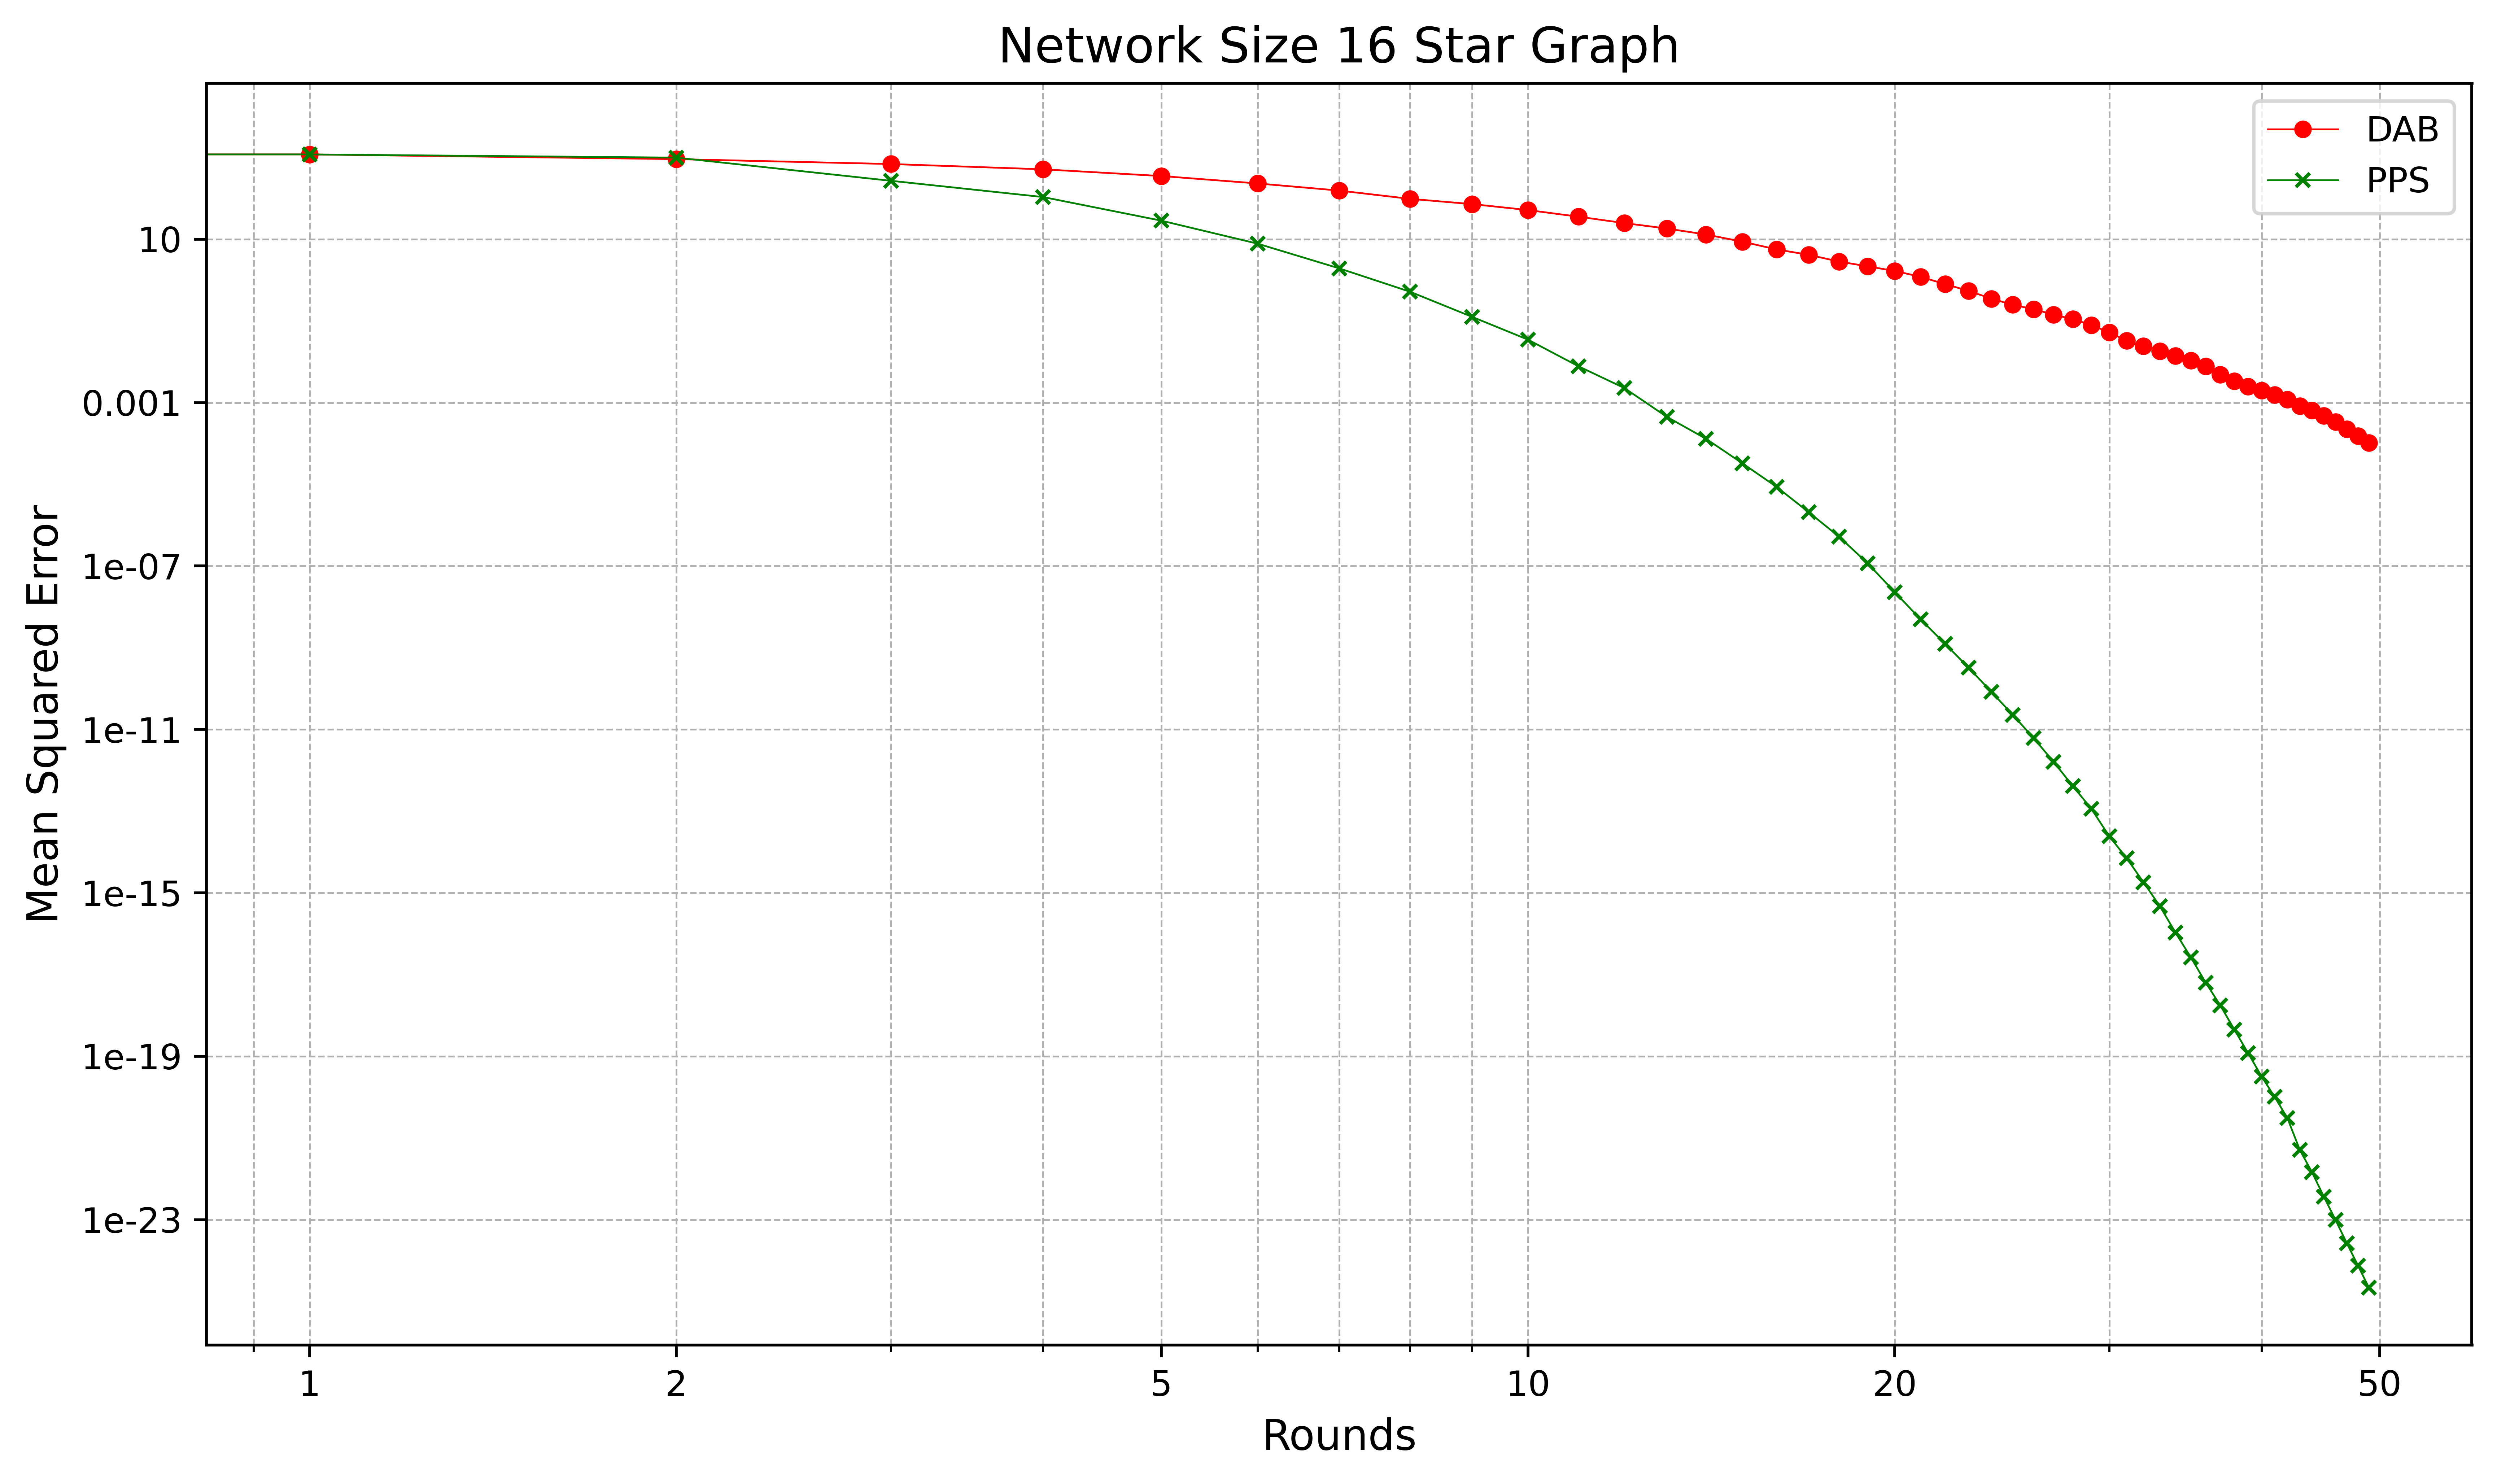
\includegraphics[scale=0.5]{figures/starGraphSimulations/DAB_vs_PPS_SG_r50_n16.png}
    \caption{Star graph: network size $2^{4}$ nodes}
    \label{fig:16StarGraph}
\end{figure}

\begin{figure}[H]
    \centering
    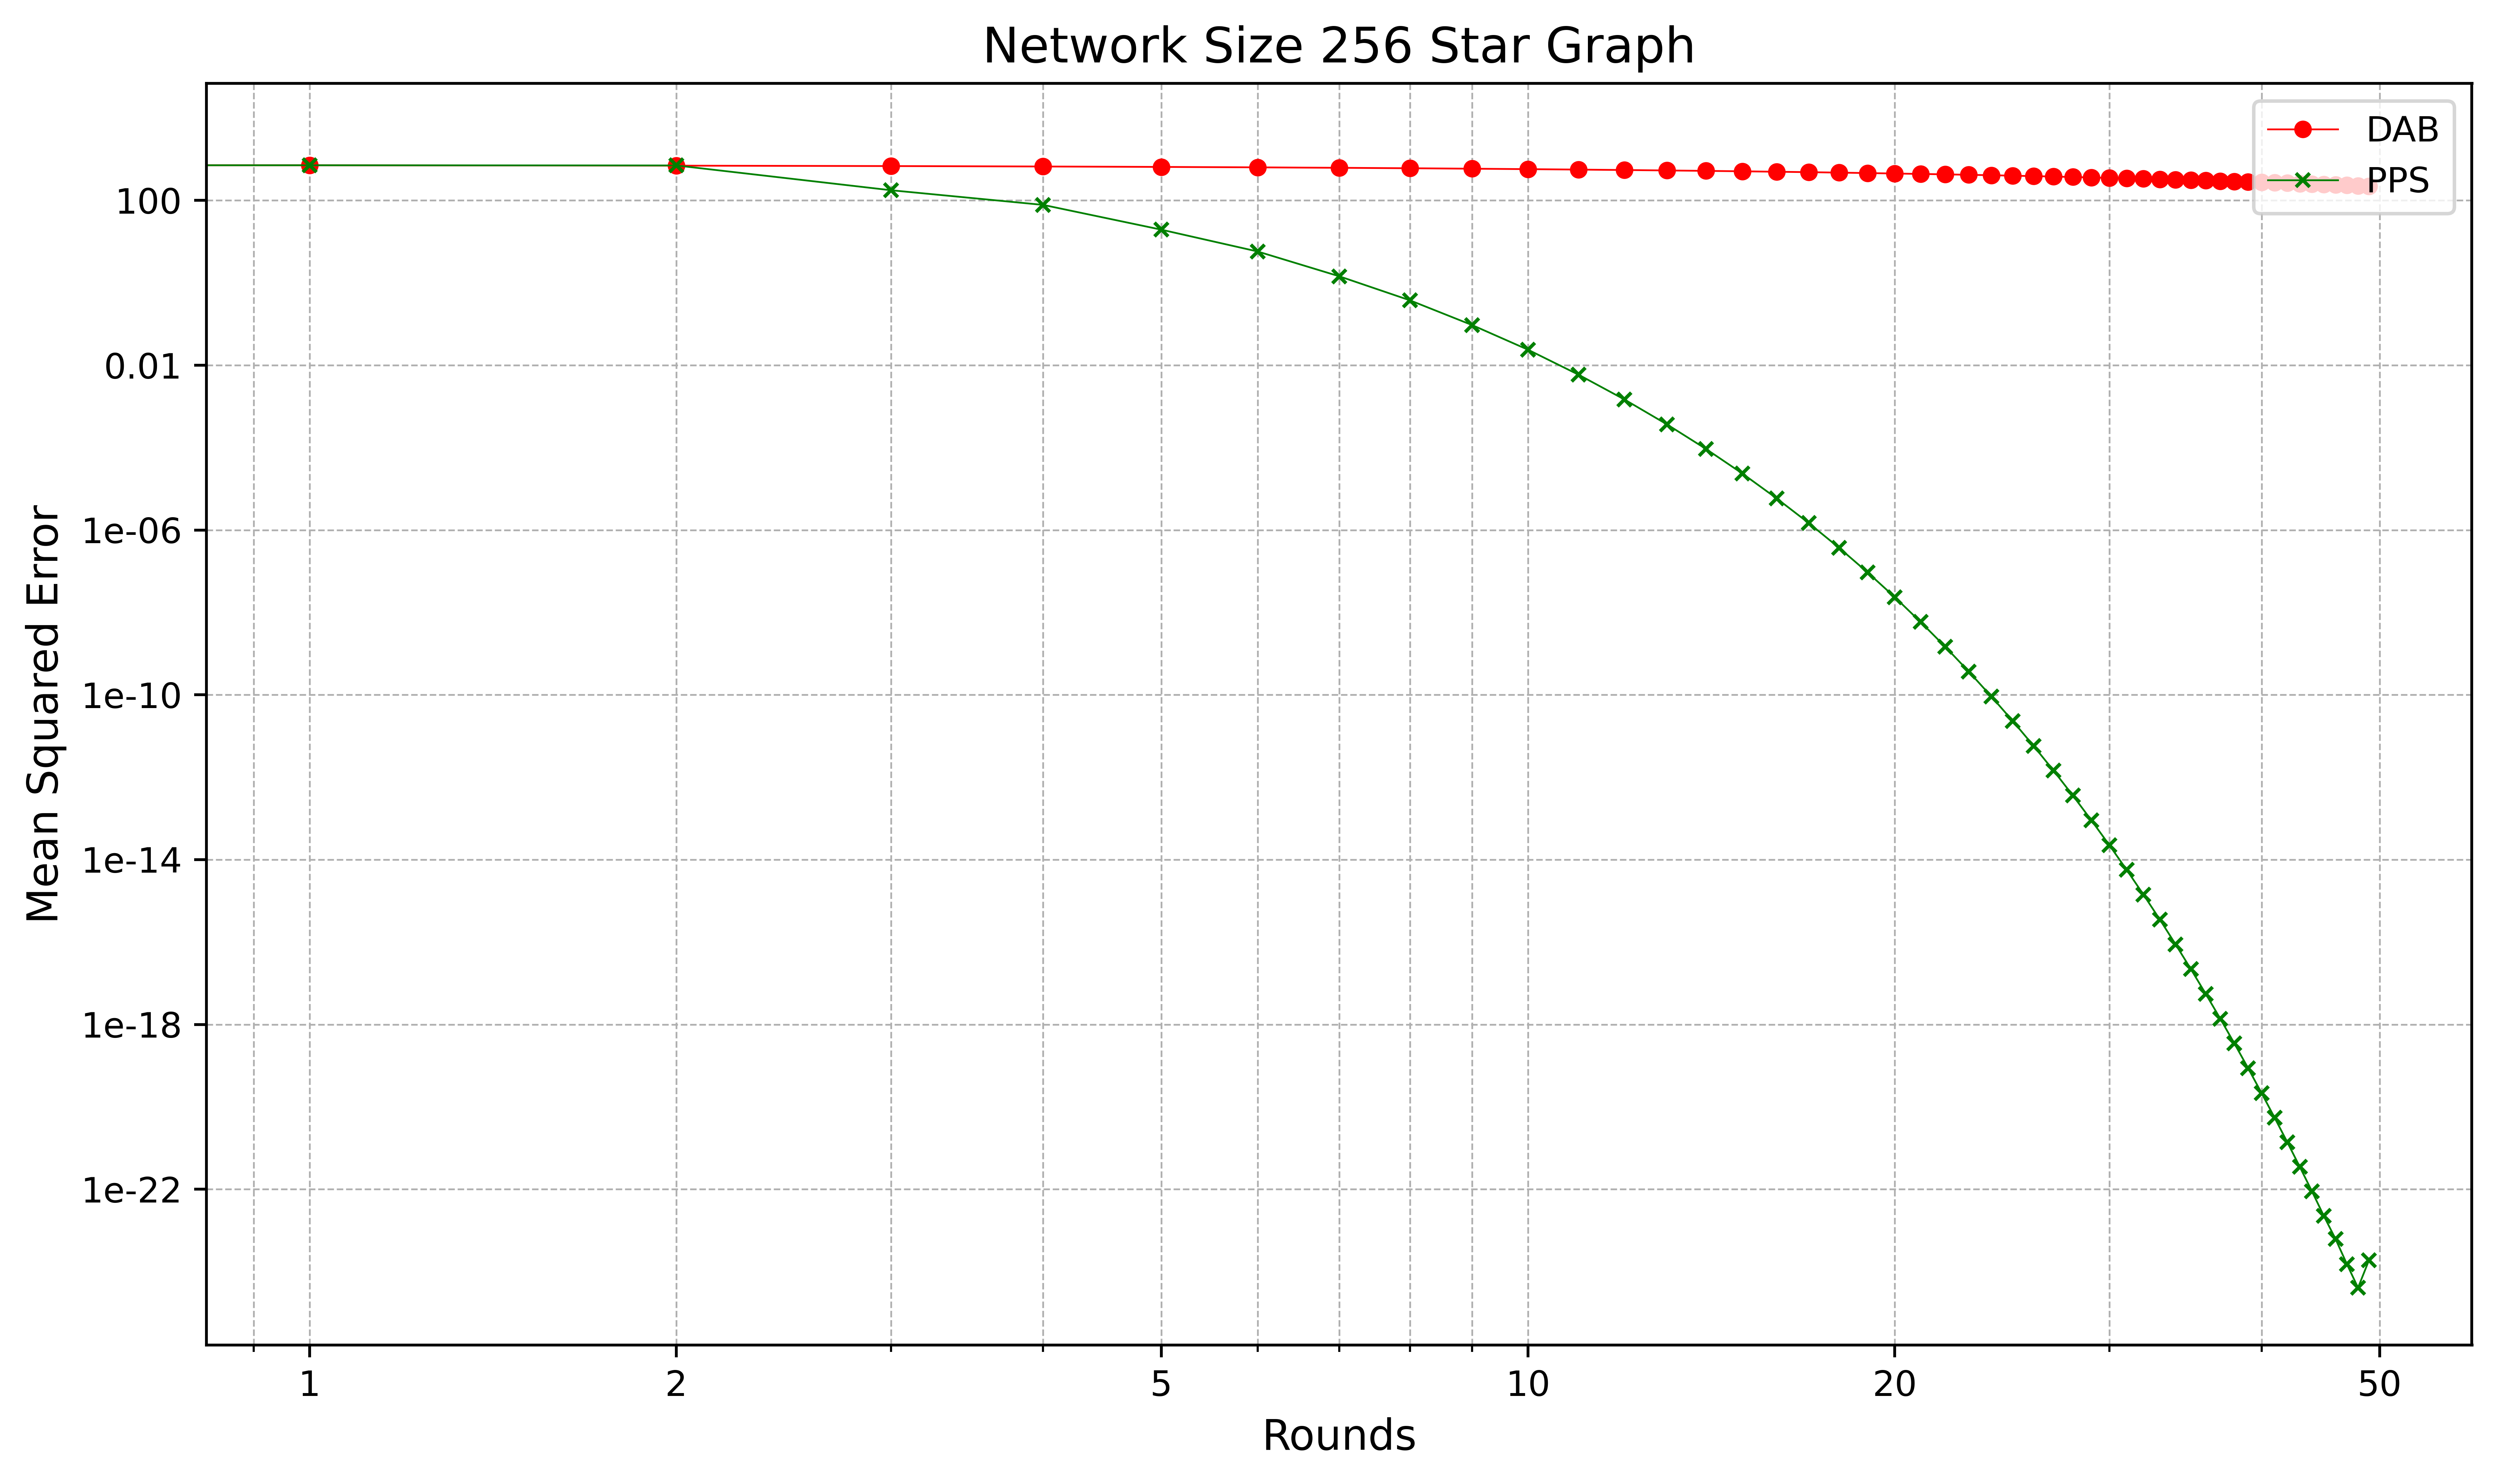
\includegraphics[scale=0.5]{figures/starGraphSimulations/DAB_vs_PPS_SG_r50_n256.png}
    \caption{Star graph: network size $2^{8}$ nodes}
    \label{fig:256StarGraph}
\end{figure}

\begin{figure}[H]
    \centering
    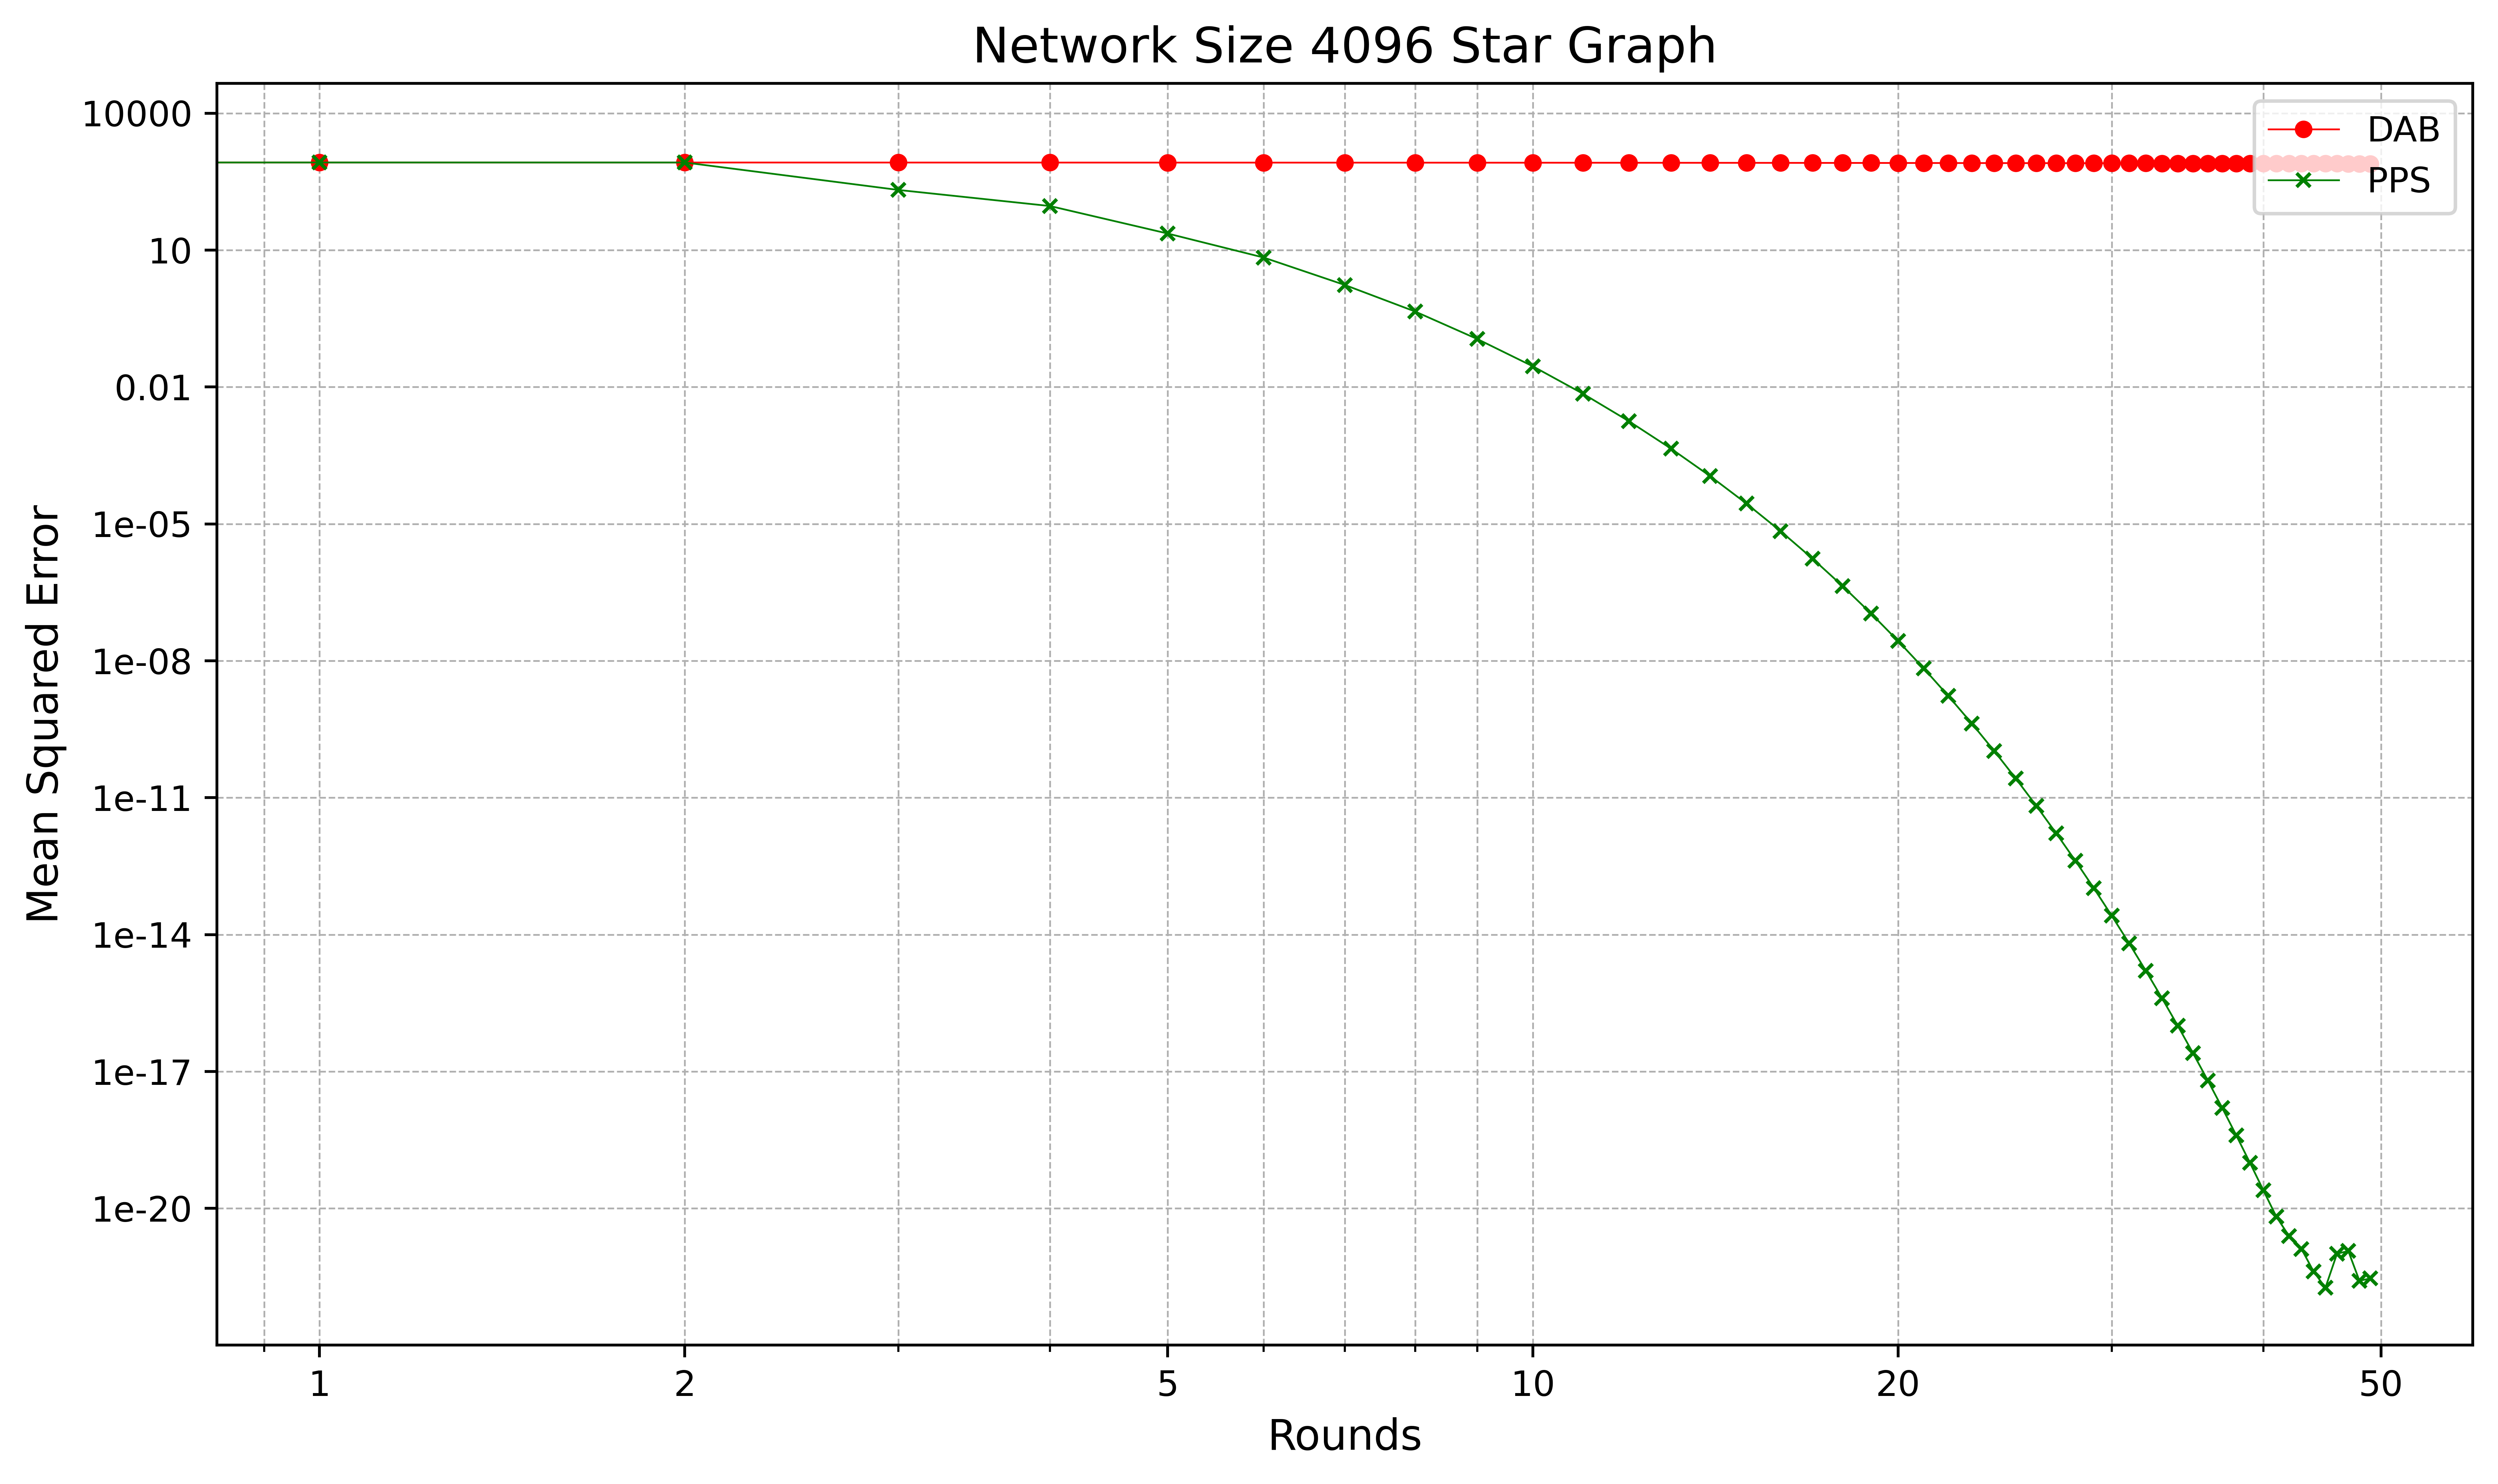
\includegraphics[scale=0.5]{figures/starGraphSimulations/DAB_vs_PPS_SG_r50_n4096.png}
    \caption{Star graph: network size $2^{12}$ nodes}
    \label{fig:4096StarGraph}
\end{figure}

\begin{figure}[H]
    \centering
    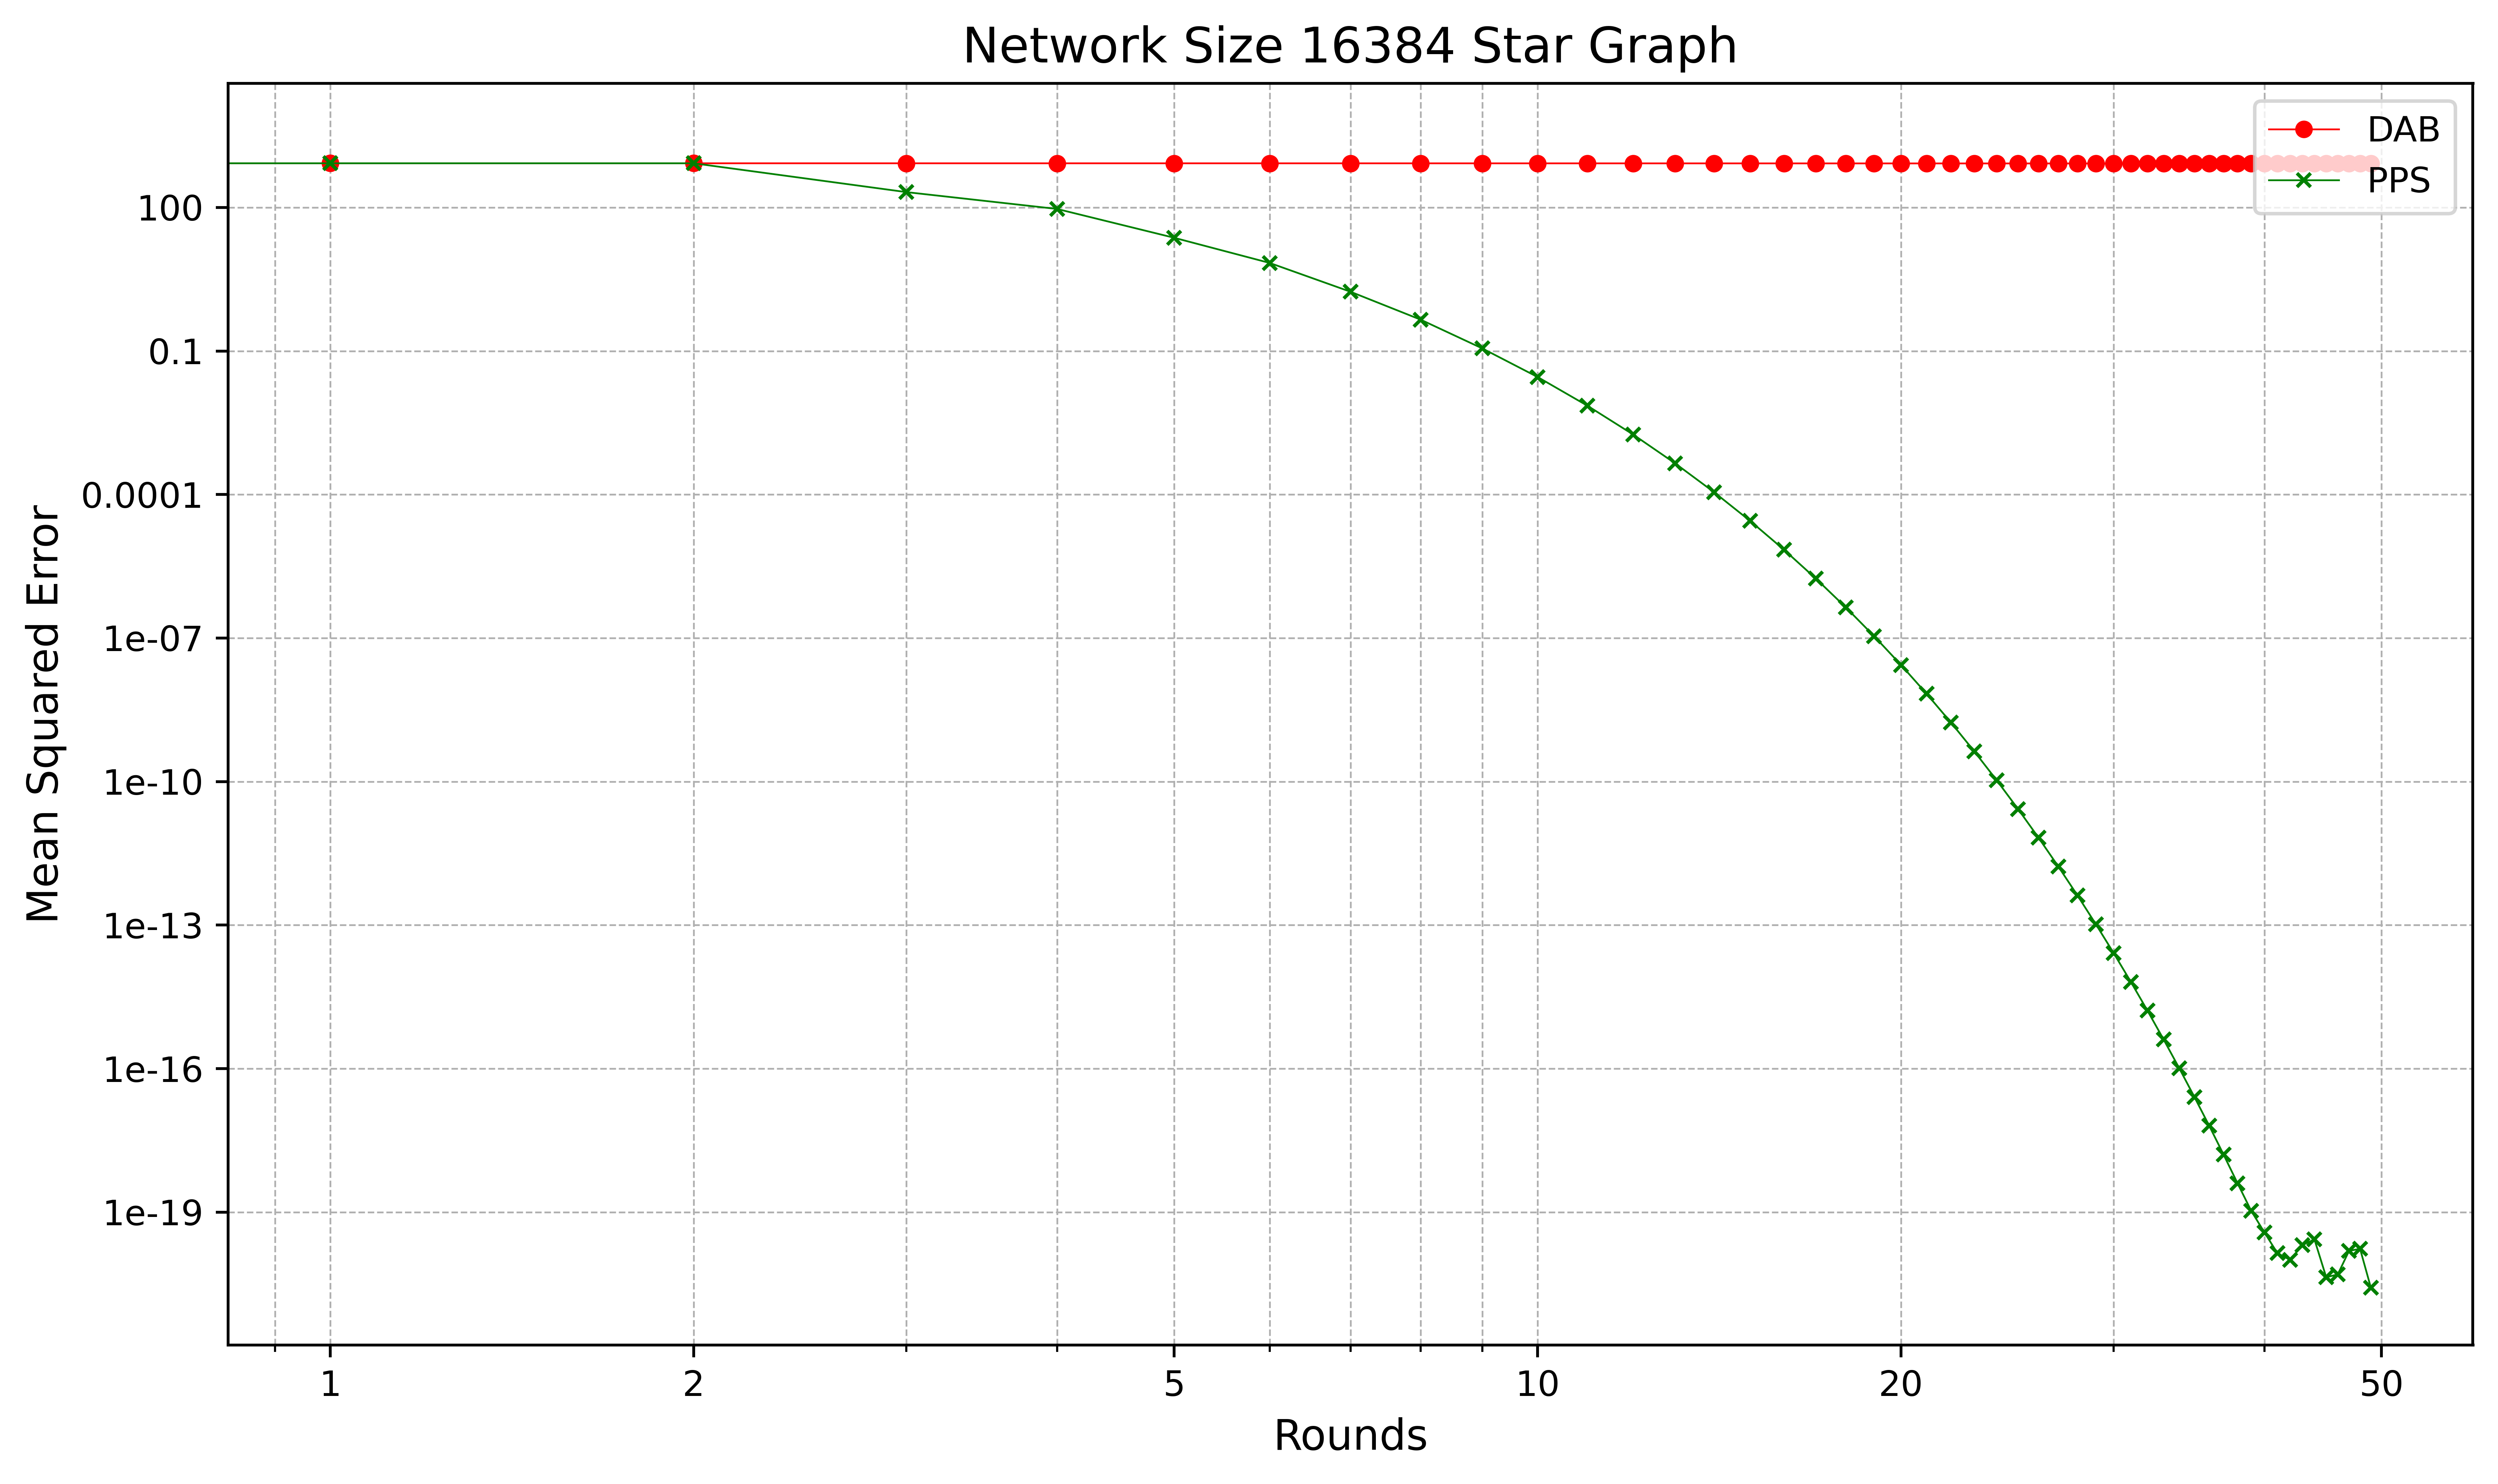
\includegraphics[scale=0.5]{figures/starGraphSimulations/DAB_vs_PPS_SG_r50_n16384.png}
    \caption{Star graph: network size $2^{14}$ nodes}
    \label{fig:16384StarGraph}
\end{figure}

\section{Closed Chain Graph}
\textbf{The closed chain graph}: A closed chain graph, also known as a closed path graph or ring, is a type of regular graph where each node has a degree of two. This means that every node is connected to exactly two other nodes. A chain graph can be drawn so that all of its vertices and edges lie on a single straight line \cite{gross1998graph}. In the case of a closed chain graph, the first and last nodes are also connected, forming a loop as depicted in \hyperref[fig:closedChainGraphDemo]{figure } \ref{fig:closedChainGraphDemo}. The graph consists of $n$ nodes and $n$ edges.
\begin{figure}[H]
    \centering
    \scalebox{0.8}{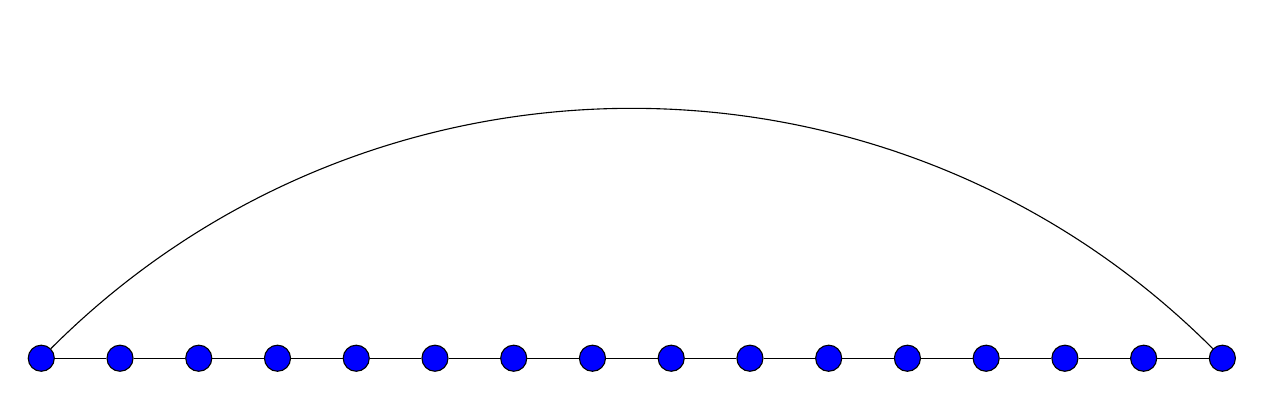
\begin{tikzpicture}
    \foreach \i in {1,...,16} {
      \node[draw, fill=blue, circle, minimum size=6pt] (v\i) at (\i, 0) {};
    }
    
    \foreach \i in {1,...,15} {
      \pgfmathtruncatemacro{\j}{\i+1}
      \draw (v\i) -- (v\j);
    }
    
    \draw[bend left=45] (v1) to (v16);
  
  \end{tikzpicture}}
    \caption{Closed chain graph: network size 16}
    \label{fig:closedChainGraphDemo}
\end{figure}
\subsection{Network sizes 2\textsuperscript{4}, 2\textsuperscript{8}, 2\textsuperscript{12} and 2\textsuperscript{14}}
\textbf{Figures}: \ref{fig:16384ChainGraph}, \ref{fig:256ChainGraph}, \ref{fig:4096ChainGraph}, \ref{fig:16384ChainGraph}\\
\textbf{Observations}: For a network size of $2^{4}$ DAB reduces the error faster than PPS within 50 rounds. The error graphs of the two protocols almost converge in the 8th round, where the MSE of the PPS balanced graph is approximately 49.41, and the MSE of the DAB balanced graph is 48.02. In the following rounds, the DAB increases its distance again. Especially after the 10th round the DAB consistently increases its lead, achieving an network with a MSE of around 0.07, while the PPS reduces the error of the network to a MSE of 0.36.

For comparison, for the network size $2^{14}$ the MSE for the PPS balanced network is about 43.72 at the end of the 50th round, whereas the DAB achieves a slightly better result for its network with an MSE of 34.88. One possible explanation for the DAB’s superior performance is the closed chain graph's structure, where each node has a degree of 2. This setup allows for exactly two possible partners for each load transfer. The PPS protocol might end up trading with a non-ideal trading partner. The DAB protocol avoids load transfers that might worsen their state locally or globally since its load transfer process is conditional. This conditional approach is the primary advantage of the DAB protocol over the PPS protocol in this scenario.\\

The DAB curve starts with a steep drop in MSE during the first few rounds and then begins to flatten as rounds increase.
This initial rapid reduction indicates that the DAB protocols converges relatively quickly at first, but then slows down, resulting in diminishing returns after the first few rounds.
This behavior suggests that the convergence follows a power law initially, but as rounds progress, the slope decreases, meaning the rate of convergence slows. The PPS curve has a slower initial downwards slope compared to DAB, but it follows a more consistent and steady reduction in MSE over time.
This means that PPS has a slower start but continues to improve steadily, whereas DAB's progress worsens after its initial fast decline.
\begin{figure}[H]
    \centering
    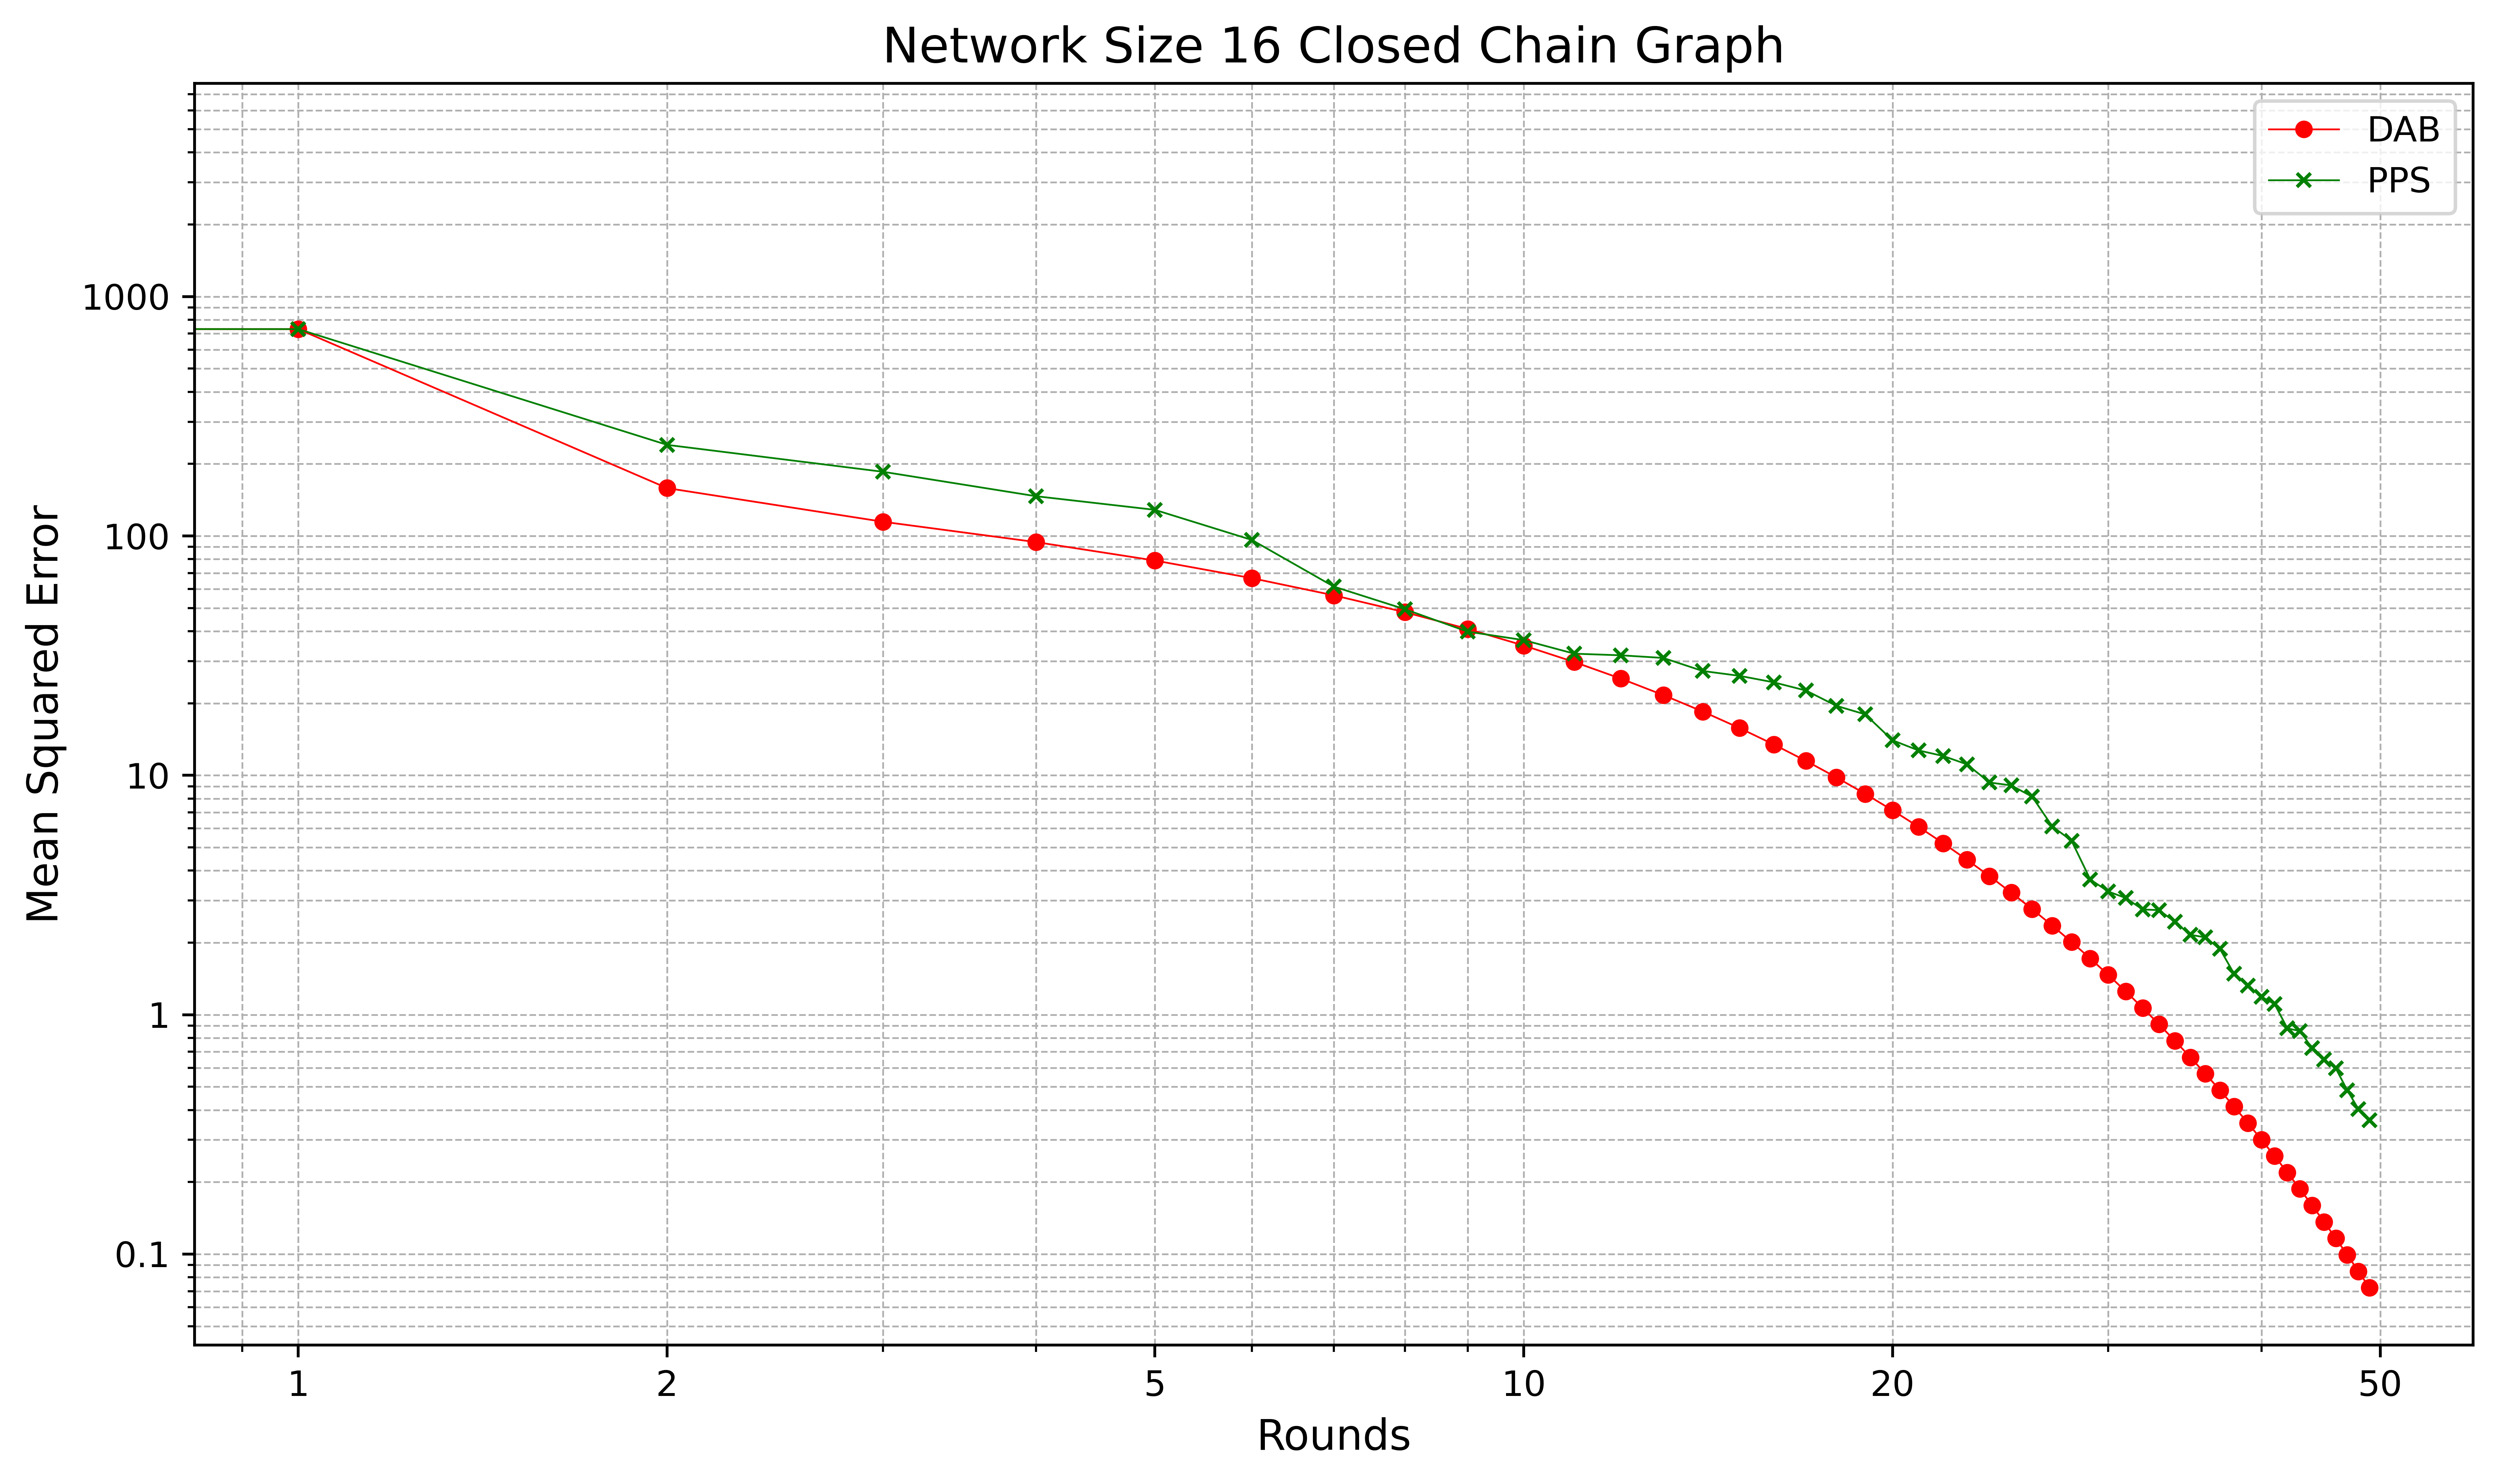
\includegraphics[scale=0.5]{figures/closedChainSimulations/DAB_vs_PPS_CCG_r50_n16.png}
    \caption{Closed chain graph: network size $2^{4}$ nodes}
    \label{fig:16ChainGraph}
\end{figure}

\begin{figure}[H]
    \centering
    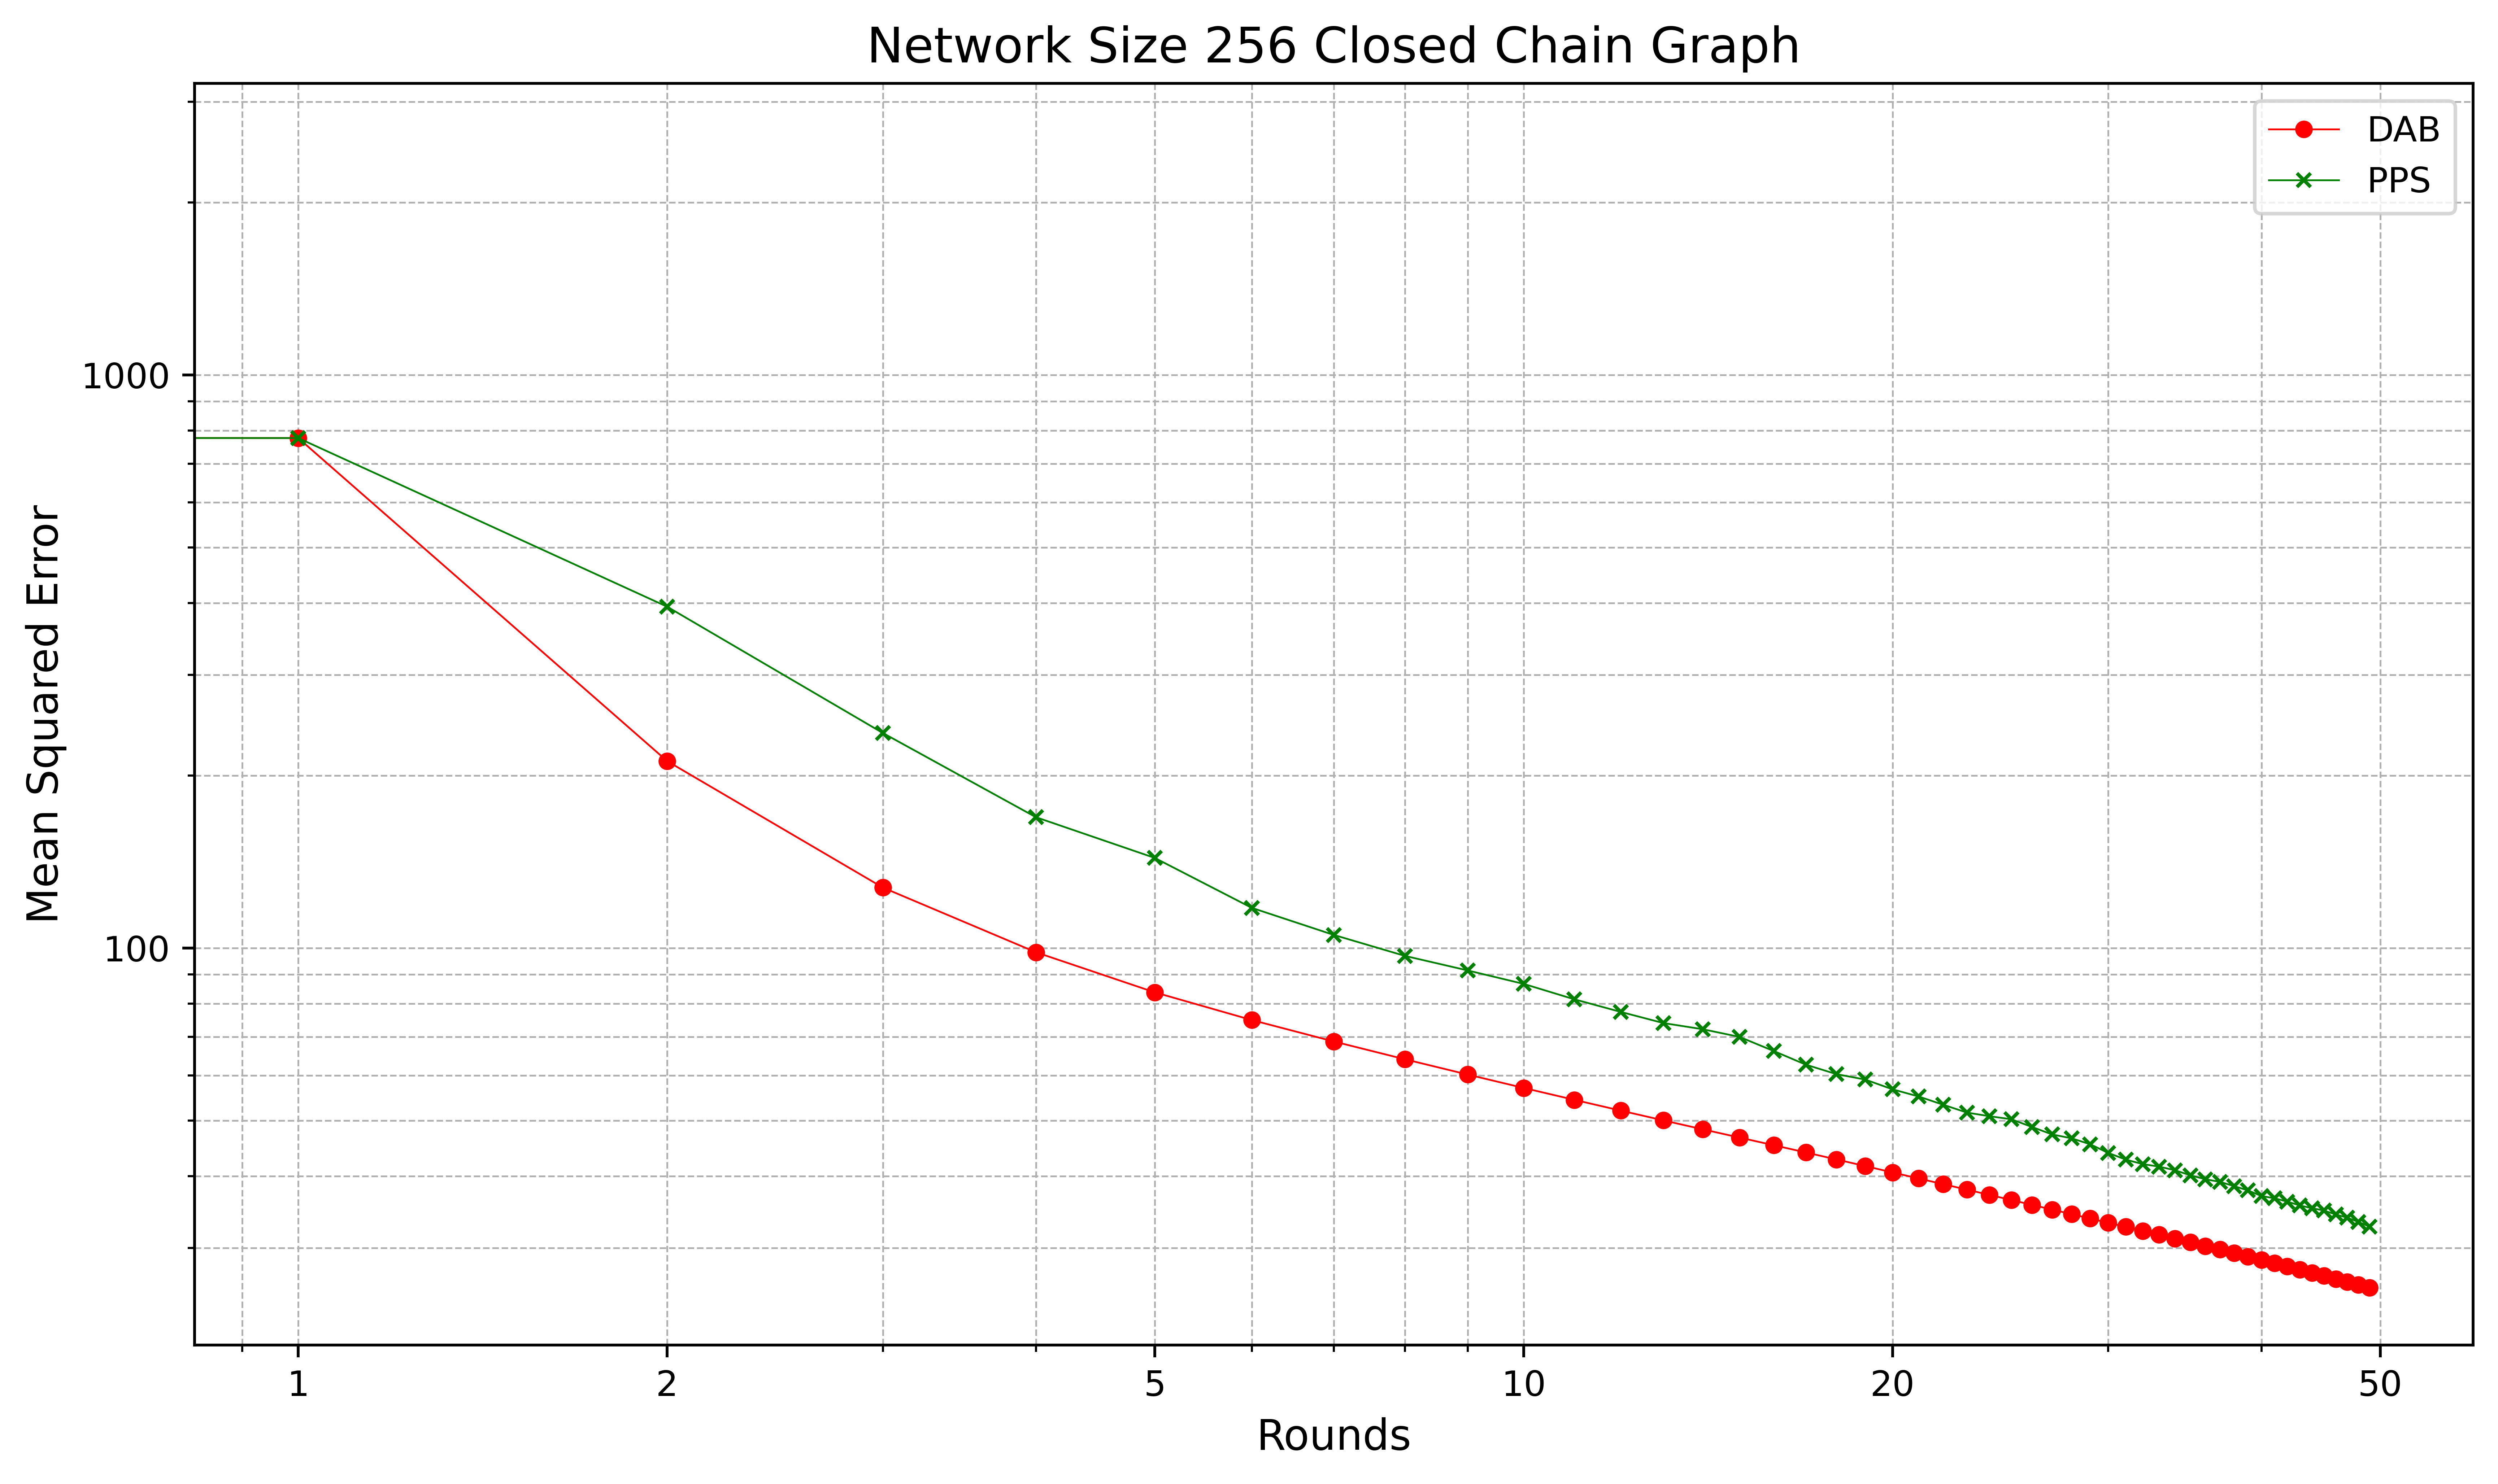
\includegraphics[scale=0.5]{figures/closedChainSimulations/DAB_vs_PPS_CCG_r50_n256.png}
    \caption{Closed chain graph: network size $2^{8}$ nodes}
    \label{fig:256ChainGraph}
\end{figure}

\begin{figure}[H]
    \centering
    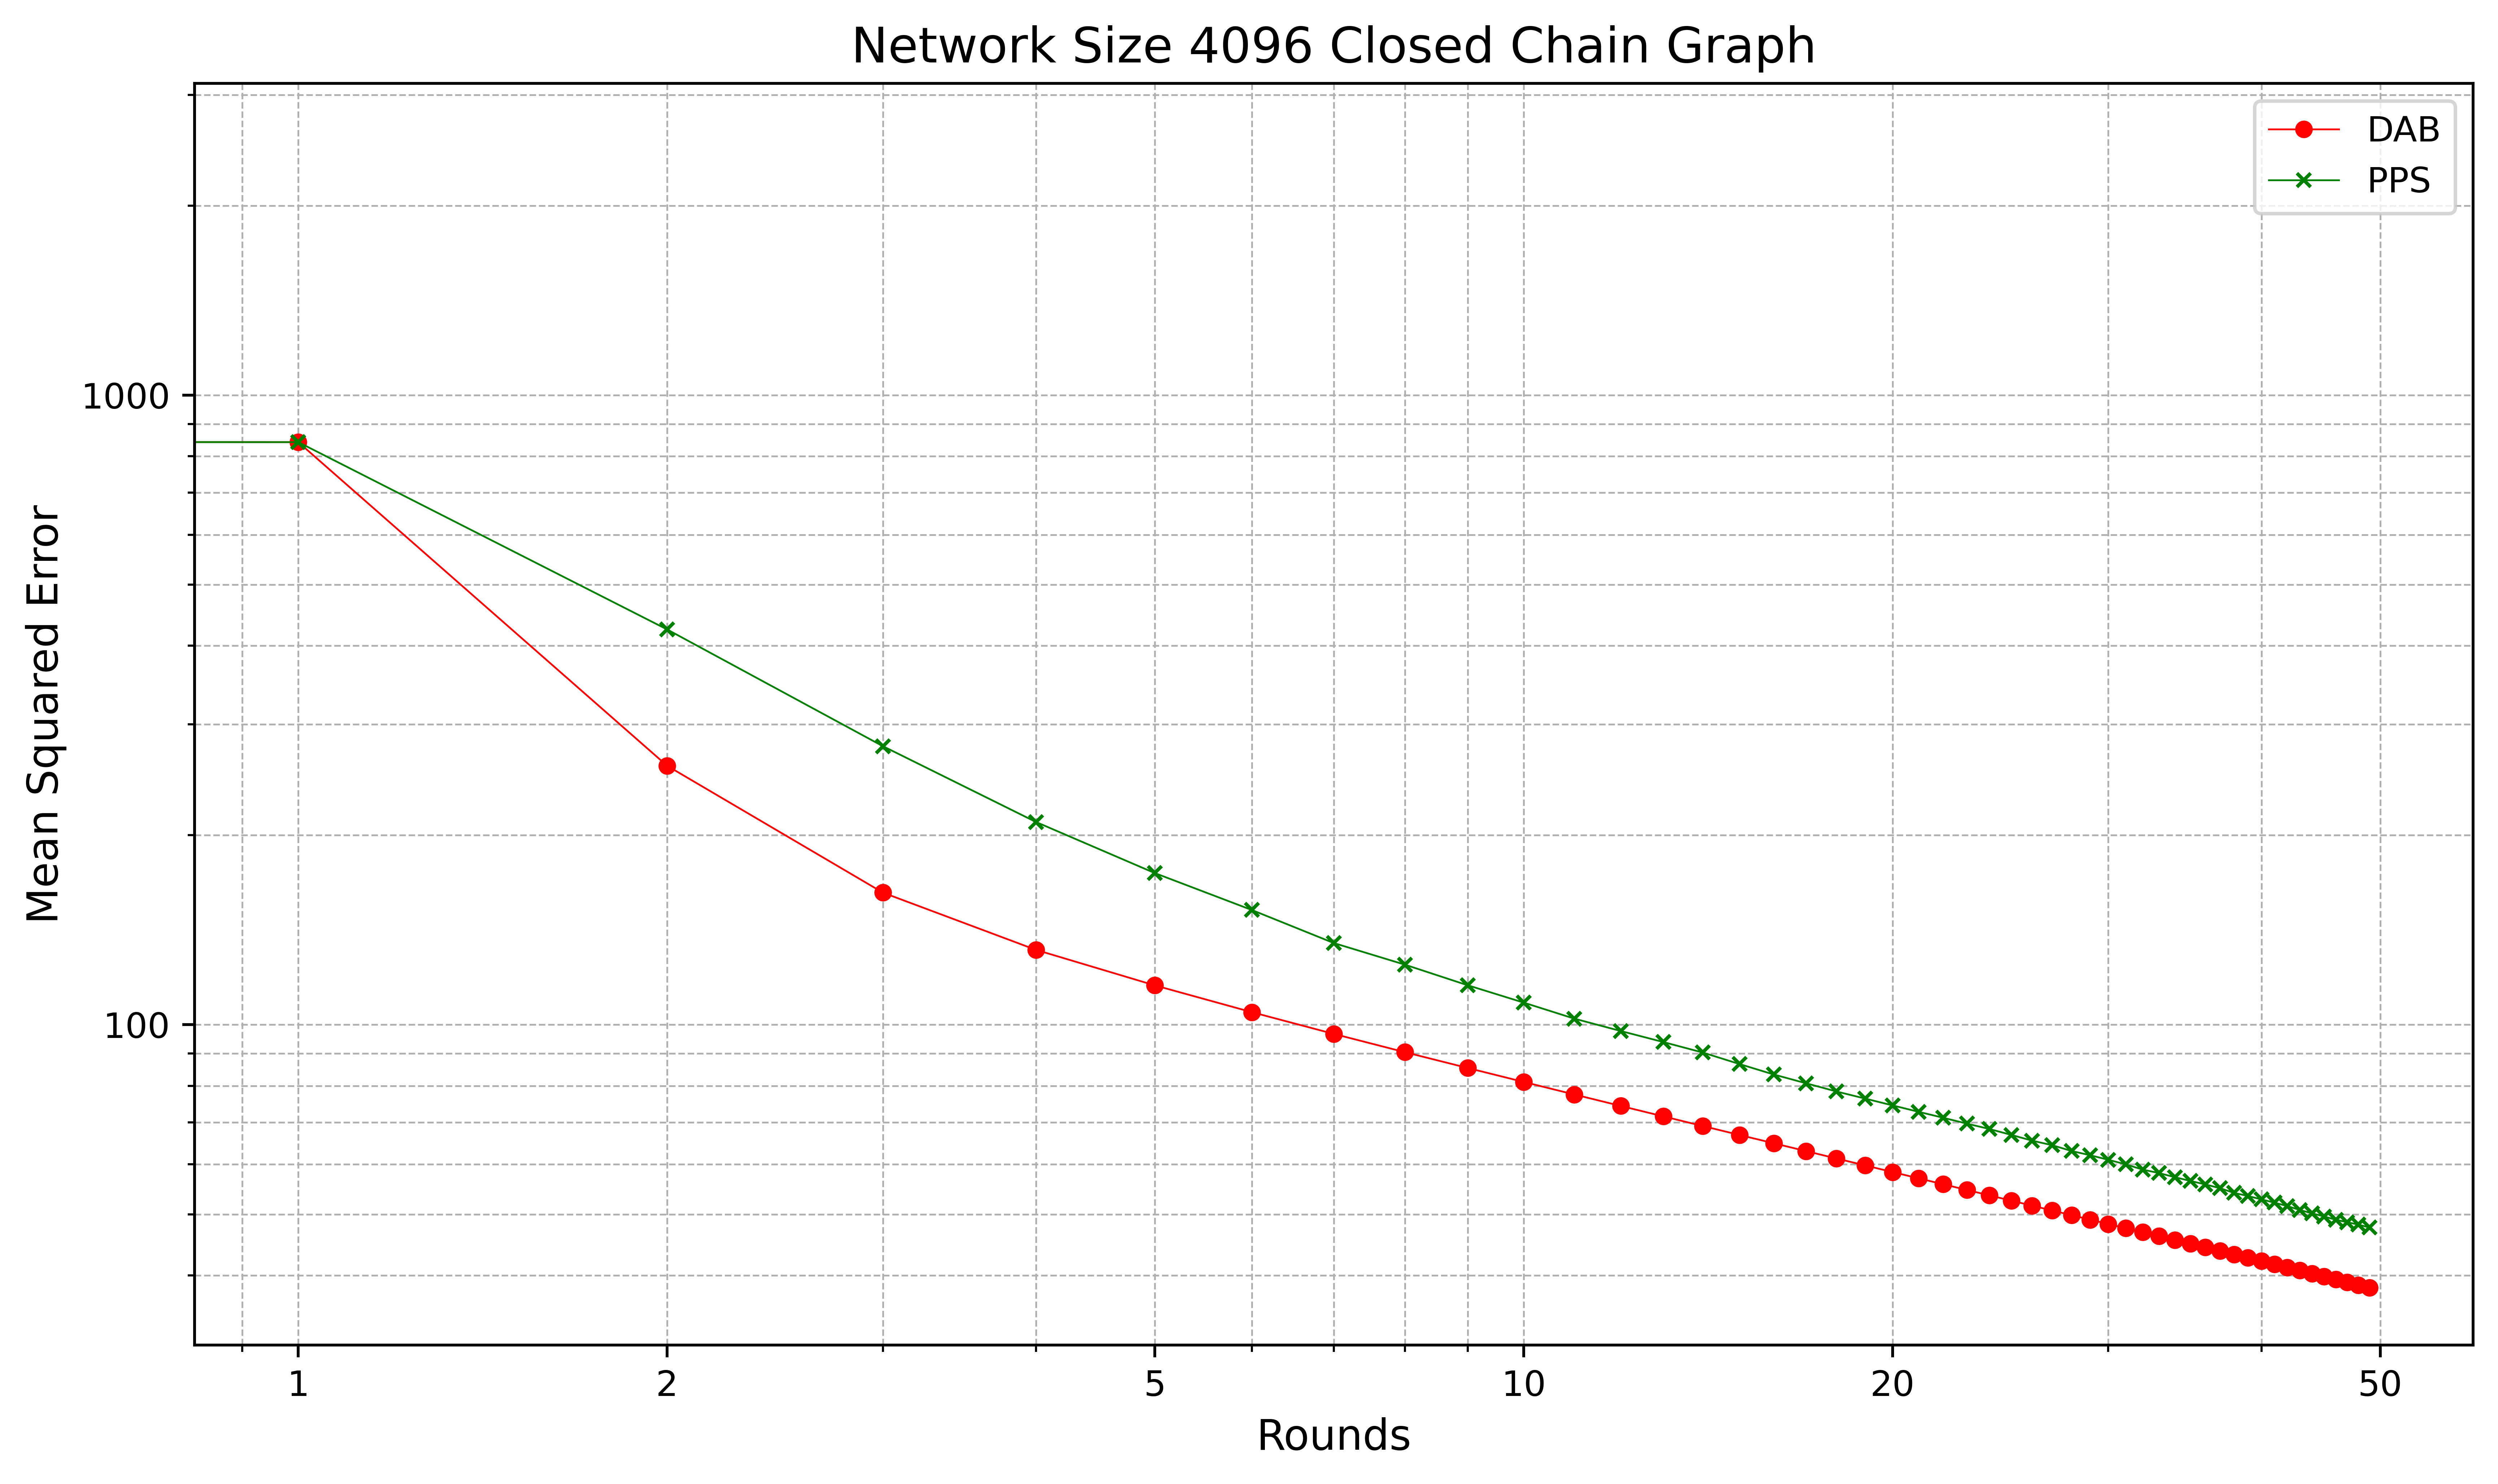
\includegraphics[scale=0.5]{figures/closedChainSimulations/DAB_vs_PPS_CCG_r50_n4096.png}
    \caption{Closed chain graph: network size $2^{12}$ nodes}
    \label{fig:4096ChainGraph}
\end{figure}

\begin{figure}[H]
    \centering
    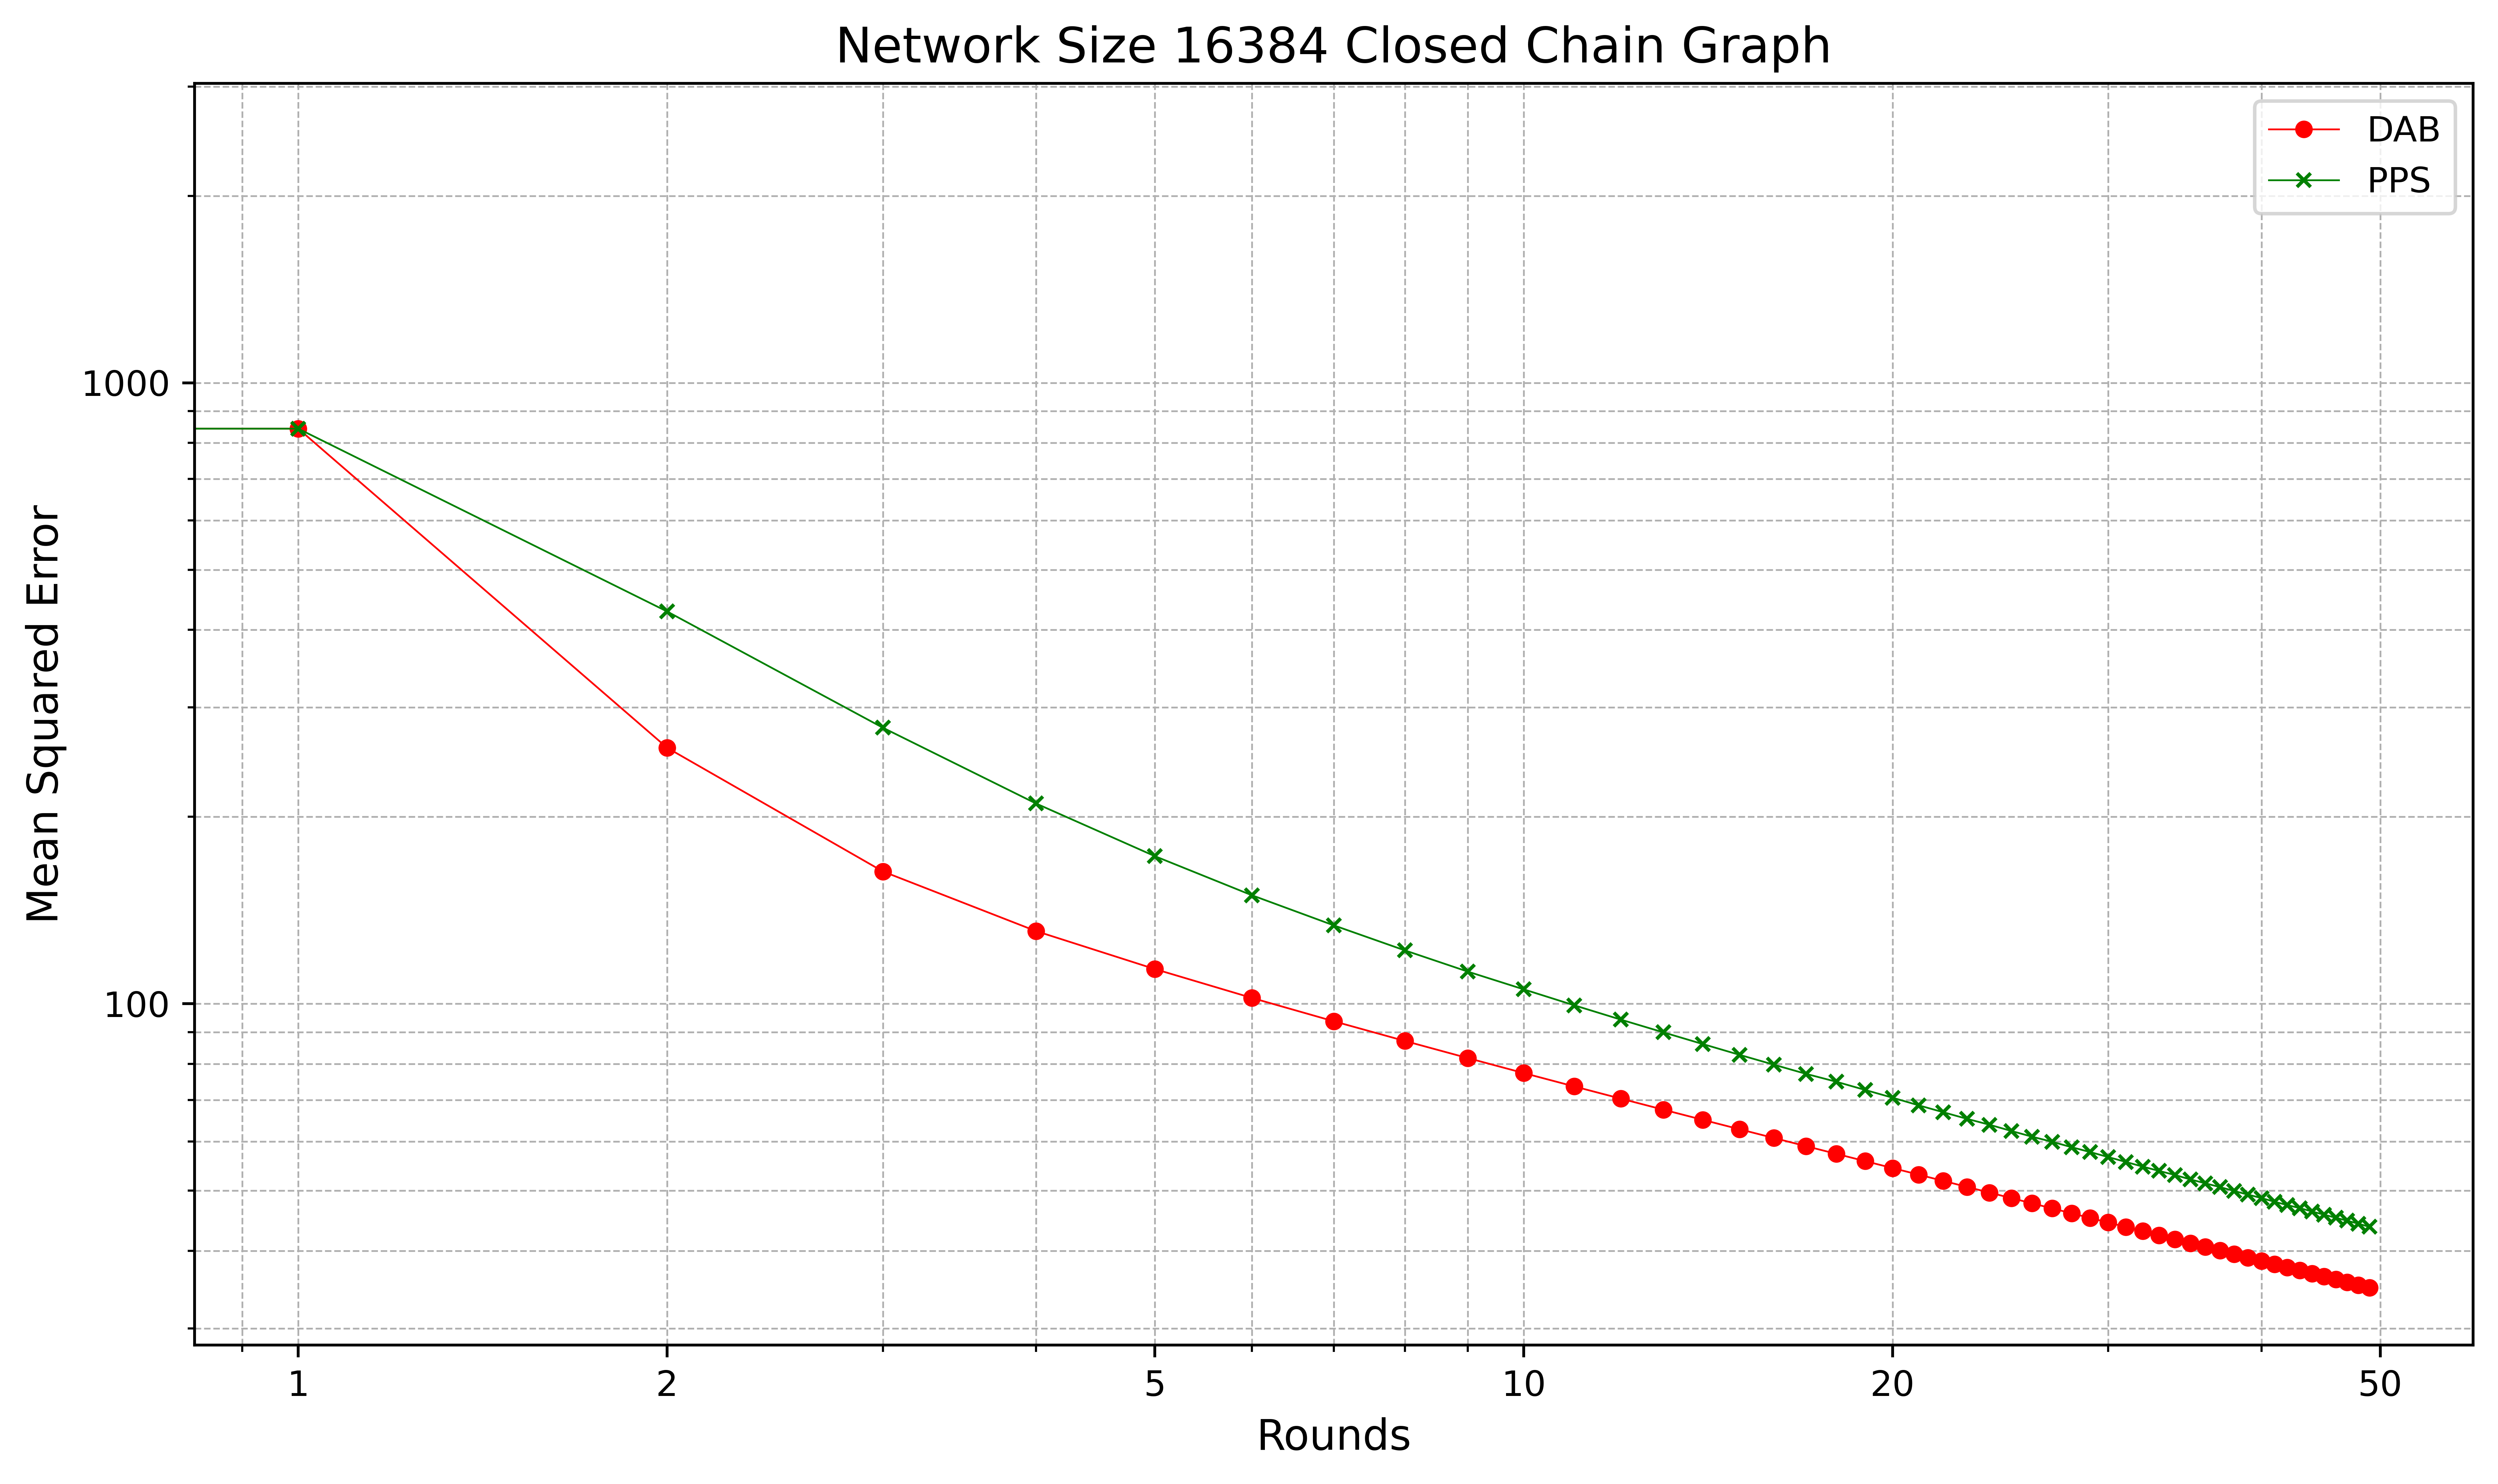
\includegraphics[scale=0.5]{figures/closedChainSimulations/DAB_vs_PPS_CCG_r50_n16384.png}
    \caption{Closed chain graph: network size $2^{14}$ nodes}
    \label{fig:16384ChainGraph}
\end{figure}

\section{Torus Grid Graph}
\textbf{The torus grid graph}: A two-dimensional torus grid graph (or sometimes solely refered to as torus) is a two-dimensional mesh with wrap around edges as depicted in \hyperref[fig:torusGraph]{figure} \ref{fig:torusGraph} \cite{Mahlmann2010}. A torus with $m \times n$ nodes where $m$ denotes the height and $n$ denotes the width, has $2\times m \times n$ edges. The torus is a regular graph, where every node has a degree of 4.

\begin{figure}[H]
    \centering
    \scalebox{1.5}{\tikzset{
    block/.style={draw, fill=blue, circle, minimum size=3pt},
    arrow/.style={->},
    line/.style={-}
}

\begin{tikzpicture}[>=stealth',node distance=0.5cm]
    % Creating rows of blocks
    {[start chain]
        \node[on chain] (s0) {};
        \node[on chain] (s1) {};
        \node[on chain] (s2) {};
        \node[on chain] (s3) {};
        \node[on chain] (s4) {};
    }
    {[start chain]
        \node[block,on chain, below = 0.15 cm of s0] (A0) {};
        \node[block,on chain, join =by {line}] (A1) {};
        \node[block,on chain, join =by {line}] (A2) {};
        \node[block,on chain, join =by {line}] (A3) {};
    }
    {[start chain]
        \node[block,on chain, below = of A0] (B0) {};
        \node[block,on chain, join =by {line}] (B1) {};
        \node[block,on chain, join =by {line}] (B2) {};
        \node[block,on chain, join =by {line}] (B3) {};
    }
    {[start chain]
        \node[block,on chain, below = of B0] (C0) {};
        \node[block,on chain, join =by {line}] (C1) {};
        \node[block,on chain, join =by {line}] (C2) {};
        \node[block,on chain, join =by {line}] (C3) {};
    }
    {[start chain]
        \node[block,on chain, below = of C0] (D0) {};
        \node[block,on chain, join =by {line}] (D1) {};
        \node[block,on chain, join =by {line}] (D2) {};
        \node[block,on chain, join =by {line}] (D3) {};
    }

    % Drawing vertical lines
    \draw (A0) -- (B0) -- (C0) -- (D0); % -- (E0);
    \draw (A1) -- (B1) -- (C1) -- (D1); % -- (E1);
    \draw (A2) -- (B2) -- (C2) -- (D2); % -- (E2);
    \draw (A3) -- (B3) -- (C3) -- (D3); % -- (E3);
    % Drawing loop backs horizontal
    \draw (A0.west) -- ($(A0.west) - (0.15, 0)$);
    \draw ($(A0.west) - (0.15, 0)$) -- ($(A0.west) - (0.15, 0)+(0,0.5)$);
    \draw ($(A0.west) - (0.15, 0)+(0,0.5)$) -- ($(A0.west) +(3.1,0.5)$);
    \draw ($(A0.west) +(3.1,0.5)$) |- (A3.east);
    % \draw (A0.north) |- (s2.north east) -| (A4.north);
    % B row
    \draw (B0.west) -- ($(B0.west) - (0.15, 0)$);
    \draw ($(B0.west) - (0.15, 0)$) -- ($(B0.west) - (0.15, 0)+(0,0.5)$);
    \draw ($(B0.west) - (0.15, 0)+(0,0.5)$) -- ($(B0.west) +(3.1,0.5)$);
    \draw ($(B0.west) +(3.1,0.5)$) |- (B3.east);
    % C row
    \draw (C0.west) -- ($(C0.west) - (0.15, 0)$);
    \draw ($(C0.west) - (0.15, 0)$) -- ($(C0.west) - (0.15, 0)+(0,0.5)$);
    \draw ($(C0.west) - (0.15, 0)+(0,0.5)$) -- ($(C0.west) +(3.1,0.5)$);
    \draw ($(C0.west) +(3.1,0.5)$) |- (C3.east);
    % D row
    \draw (D0.west) -- ($(D0.west) - (0.15, 0)$);
    \draw ($(D0.west) - (0.15, 0)$) -- ($(D0.west) - (0.15, 0)+(0,0.5)$);
    \draw ($(D0.west) - (0.15, 0)+(0,0.5)$) -- ($(D0.west) +(3.1,0.5)$);
    \draw ($(D0.west) +(3.1,0.5)$) |- (D3.east);

    % Vertical Loopbacks

    % 0 column
    \draw (A0.north) -- ($(A0.north) + (0.0, 0.15)$);
    \draw ($(A0.north) + (0, 0.15)$) -- ($(A0.north) + (0, 0.15)+(-0.5,0)$);
    \draw ($(A0.north) + (0, 0.15)+(-0.5,0)$) -- ($(D0.north) +(-0.5,-0.65)$);
    \draw ($(D0.north) +(-0.5,-0.65)$) -| (D0.south);
    % 1 column
    \draw (A1.north) -- ($(A1.north) + (0.0, 0.15)$);
    \draw ($(A1.north) + (0, 0.15)$) -- ($(A1.north) + (0, 0.15)+(-0.5,0)$);
    \draw ($(A1.north) + (0, 0.15)+(-0.5,0)$) -- ($(D1.north) +(-0.5,-0.65)$);
    \draw ($(D1.north) +(-0.5,-0.65)$) -| (D1.south);
    % 2 column
    \draw (A2.north) -- ($(A2.north) + (0.0, 0.15)$);
    \draw ($(A2.north) + (0, 0.15)$) -- ($(A2.north) + (0, 0.15)+(-0.5,0)$);
    \draw ($(A2.north) + (0, 0.15)+(-0.5,0)$) -- ($(D2.north) +(-0.5,-0.65)$);
    \draw ($(D2.north) +(-0.5,-0.65)$) -| (D2.south);

    % 3 column
    \draw (A3.north) -- ($(A3.north) + (0.0, 0.15)$);
    \draw ($(A3.north) + (0, 0.15)$) -- ($(A3.north) + (0, 0.15)+(-0.5,0)$);
    \draw ($(A3.north) + (0, 0.15)+(-0.5,0)$) -- ($(D3.north) +(-0.5,-0.65)$);
    \draw ($(D3.north) +(-0.5,-0.65)$) -| (D3.south);
    
    \end{tikzpicture}}
    \caption{Torus grid graph: network size 16}
    \label{fig:torusGraph}
\end{figure}

\subsection{Network sizes: 2\textsuperscript{4}, 2\textsuperscript{8}, 2\textsuperscript{12}}
\textbf{Figures}: \ref{fig:16torusGraph}, \ref{fig:256torusGraph}, \ref{fig:4096torusGraph}\\
\textbf{Observations}: For the network sizes $2^{4}$, $2^{8}$ and $2^{12}$ DAB performs better than the PPS, although the difference in MSE of the two networks diminishes as the network size increases. For a network size of $2^{4}$ the DAB was actually able to balance the whole network by round 17. The MSE decreases to zero, achieving a perfectly balanced network. The PPS also perfoms good, reducing the error to approximately $6.68e-15$ by round 50.

For the network size $2^{8}$ DAB reduces the MSE of its network to nearly 0.04 by the end of round 50, while the PPS achieves a MSE of 1.5 in its network. For a network size $2^{12}$ the difference between the networks balanced by the protocols becomes less significant. The DAB protocol achieves an MSE of 1.66 in its network, compared to the PPS's networks MSE of 3.59.

This observation can be explained by the fact that nodes in the torus graph always have exactly 4 neighbours (due to the regularity of the graph). This low connectivity increases the likelihood that a node of the PPS might not find an optimal trading partner, and therefore increase the local error. In contrast, the DAB protocol's controlled and conditional load distribution proves more efficient in graphs with lower connectivity.

The decreasing slope over time suggests that DAB has a diminishing effect: initially very effective, but unable to maintain its improvement from the first few rounds. However, the slope of the PPS curve is more consistent, showing that PPS steadily reduces the MSE of its network, though at a slower rate initially compared to DAB.\\
\begin{figure}[H]
    \centering
    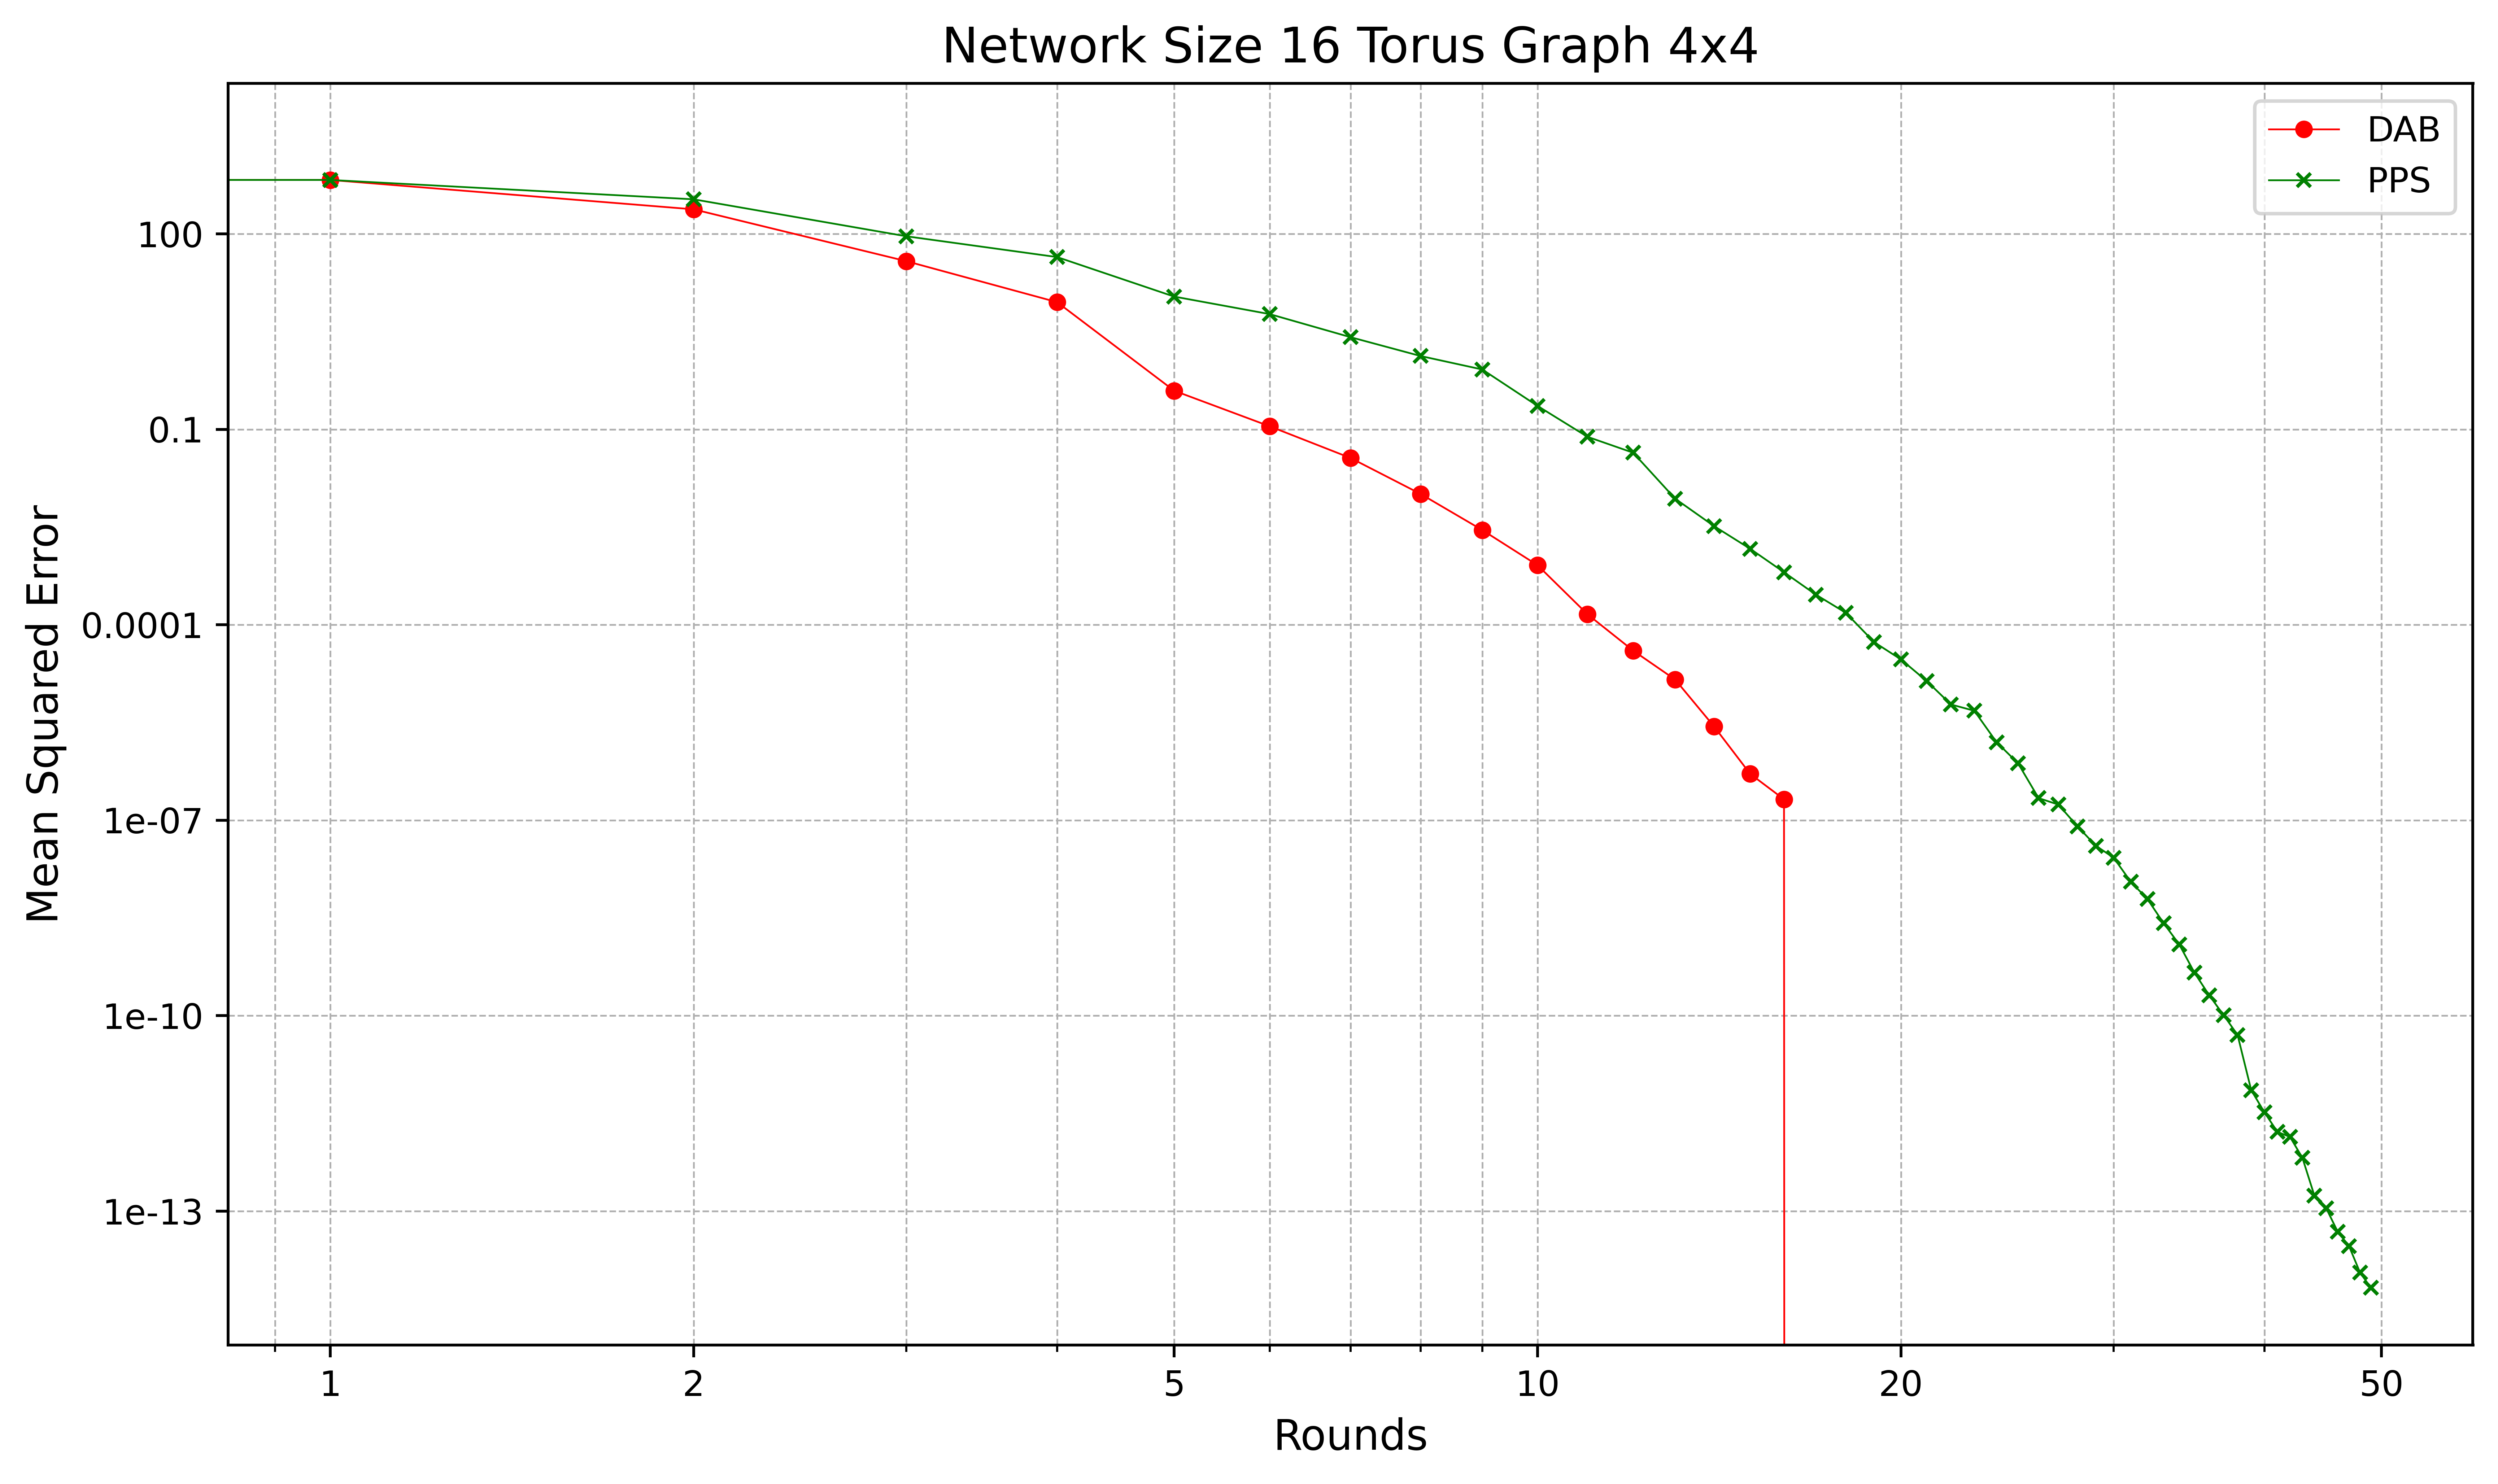
\includegraphics[scale=0.5]{figures/torusGridGraphSimulations/DAB_vs_PPS_TG_r50_n16.png}
    \caption{Torus grid graph: network size $2^{4}$}
    \label{fig:16torusGraph}
\end{figure}

\begin{figure}[H]
    \centering
    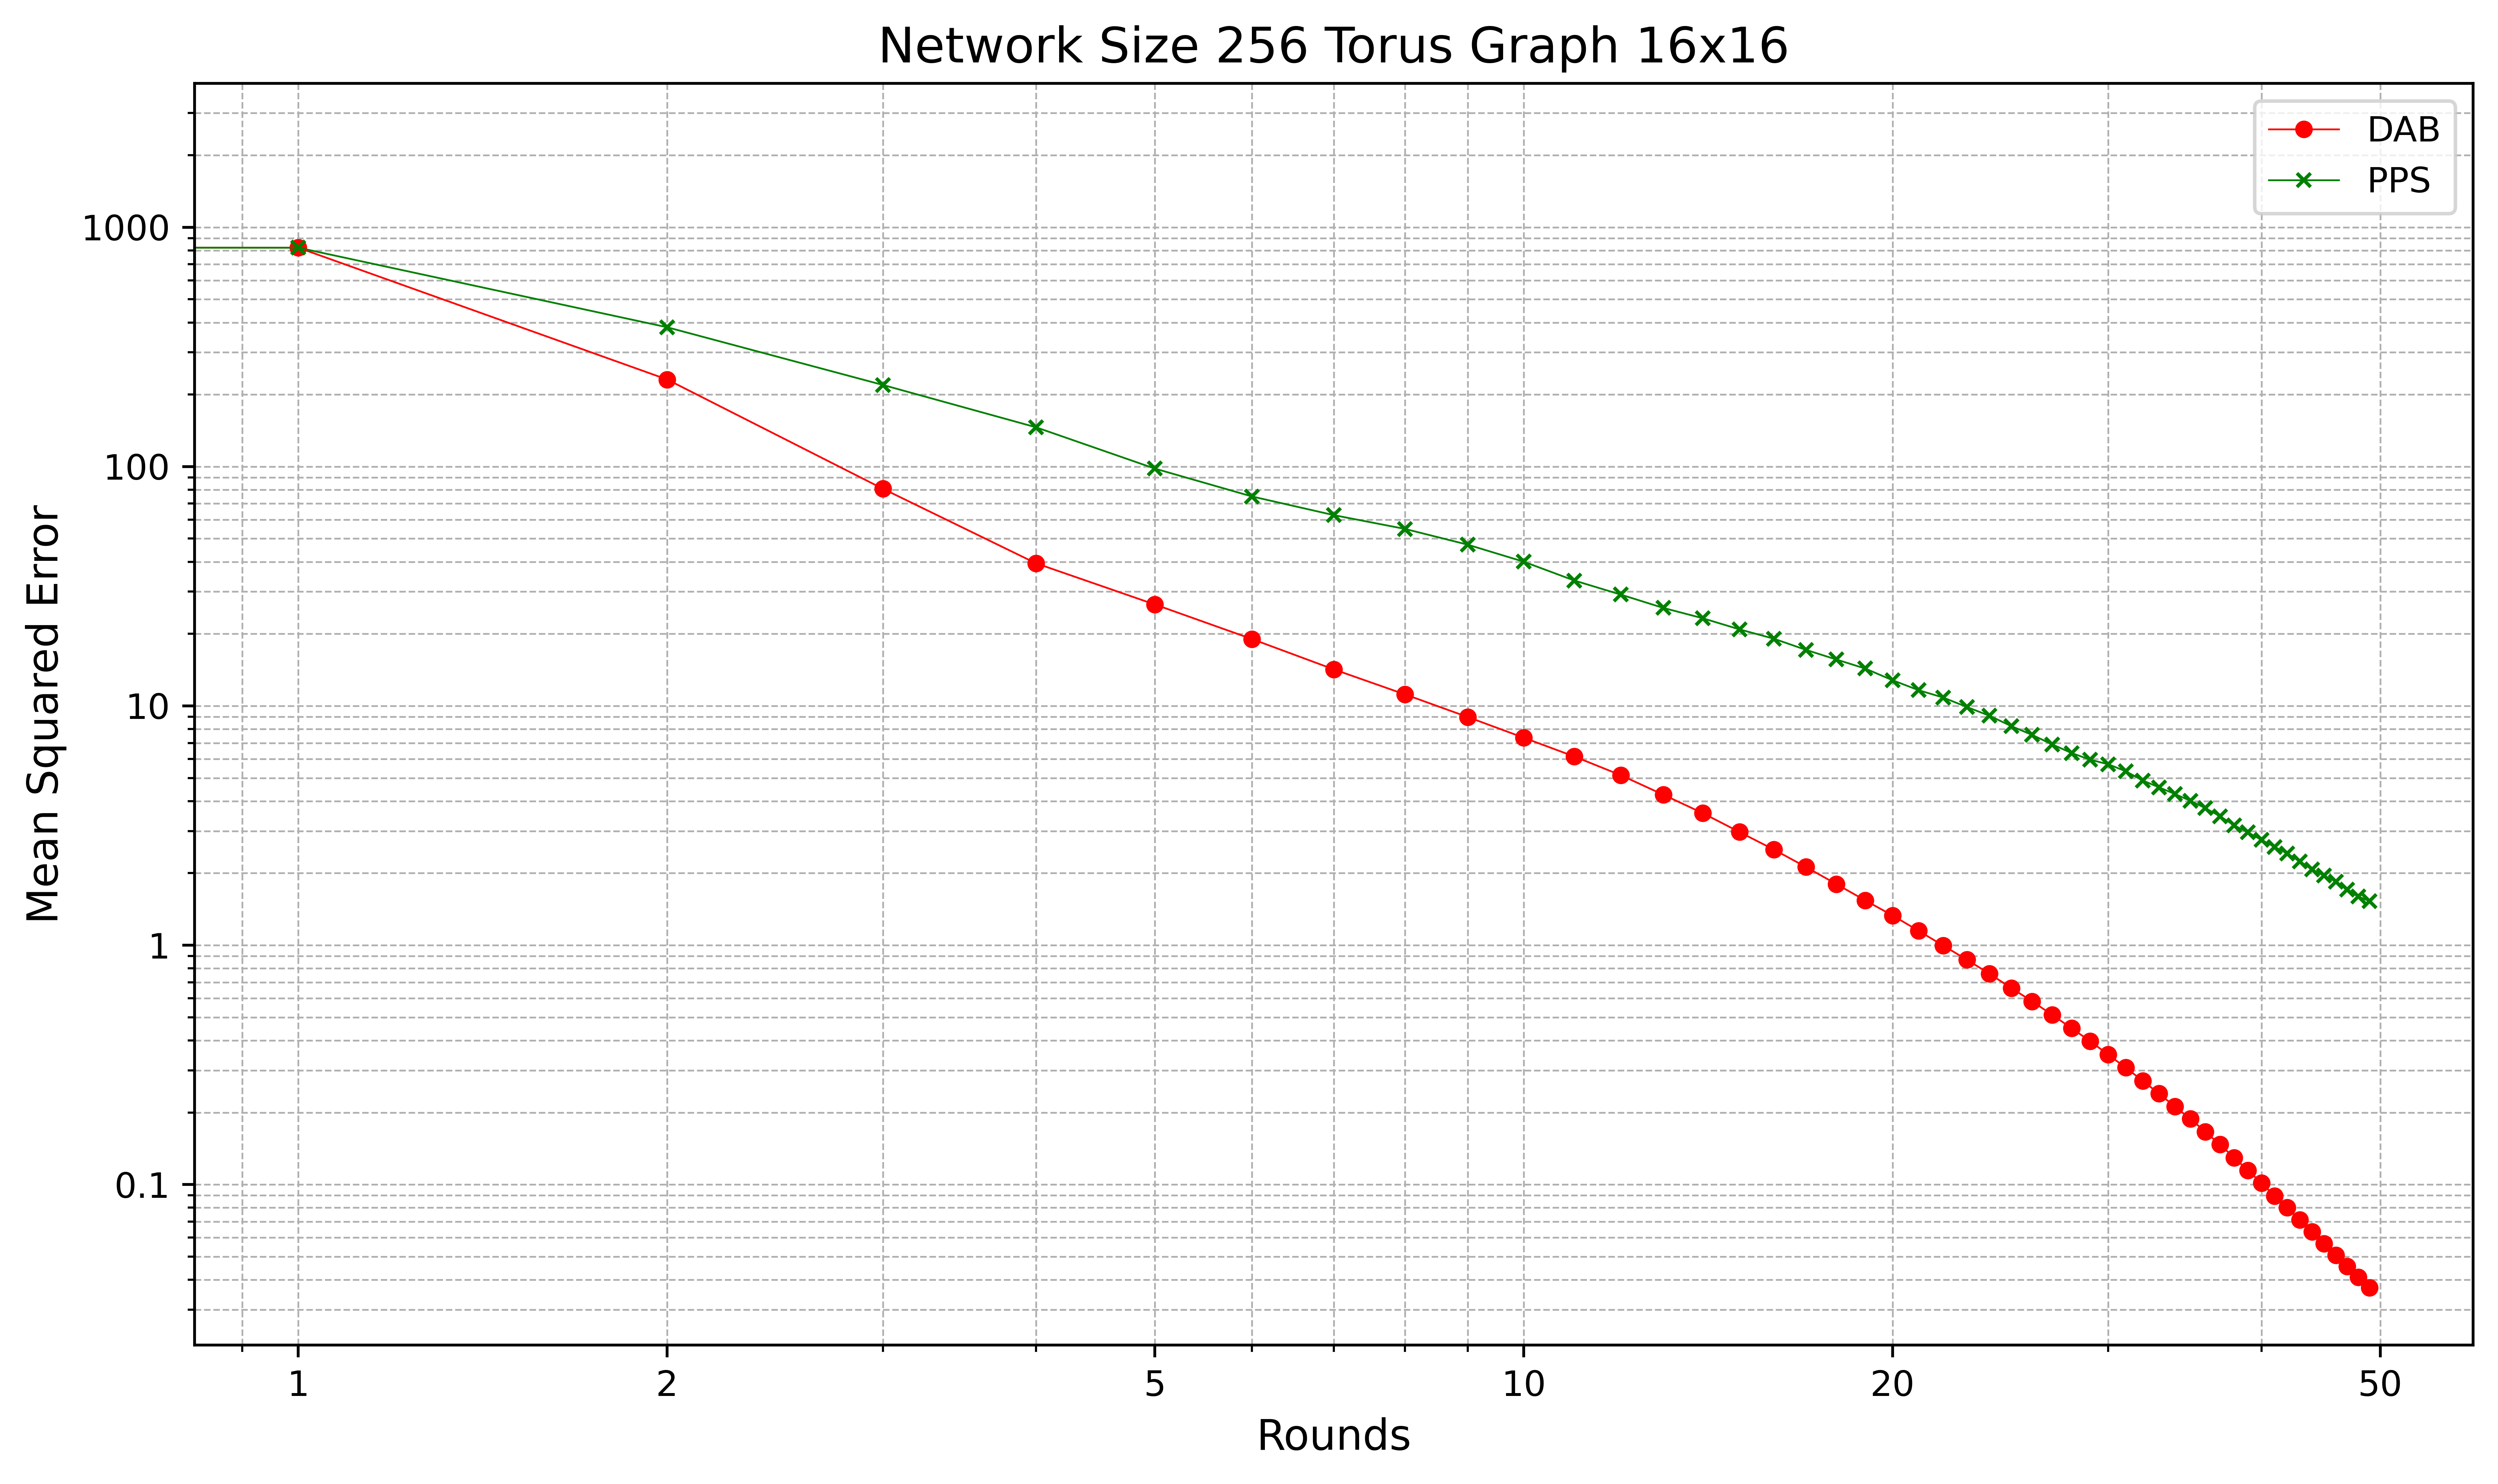
\includegraphics[scale=0.5]{figures/torusGridGraphSimulations/DAB_vs_PPS_TG_r50_n256.png}
    \caption{Torus grid graph: network size $2^{8}$}
    \label{fig:256torusGraph}
\end{figure}

\begin{figure}[H]
    \centering
    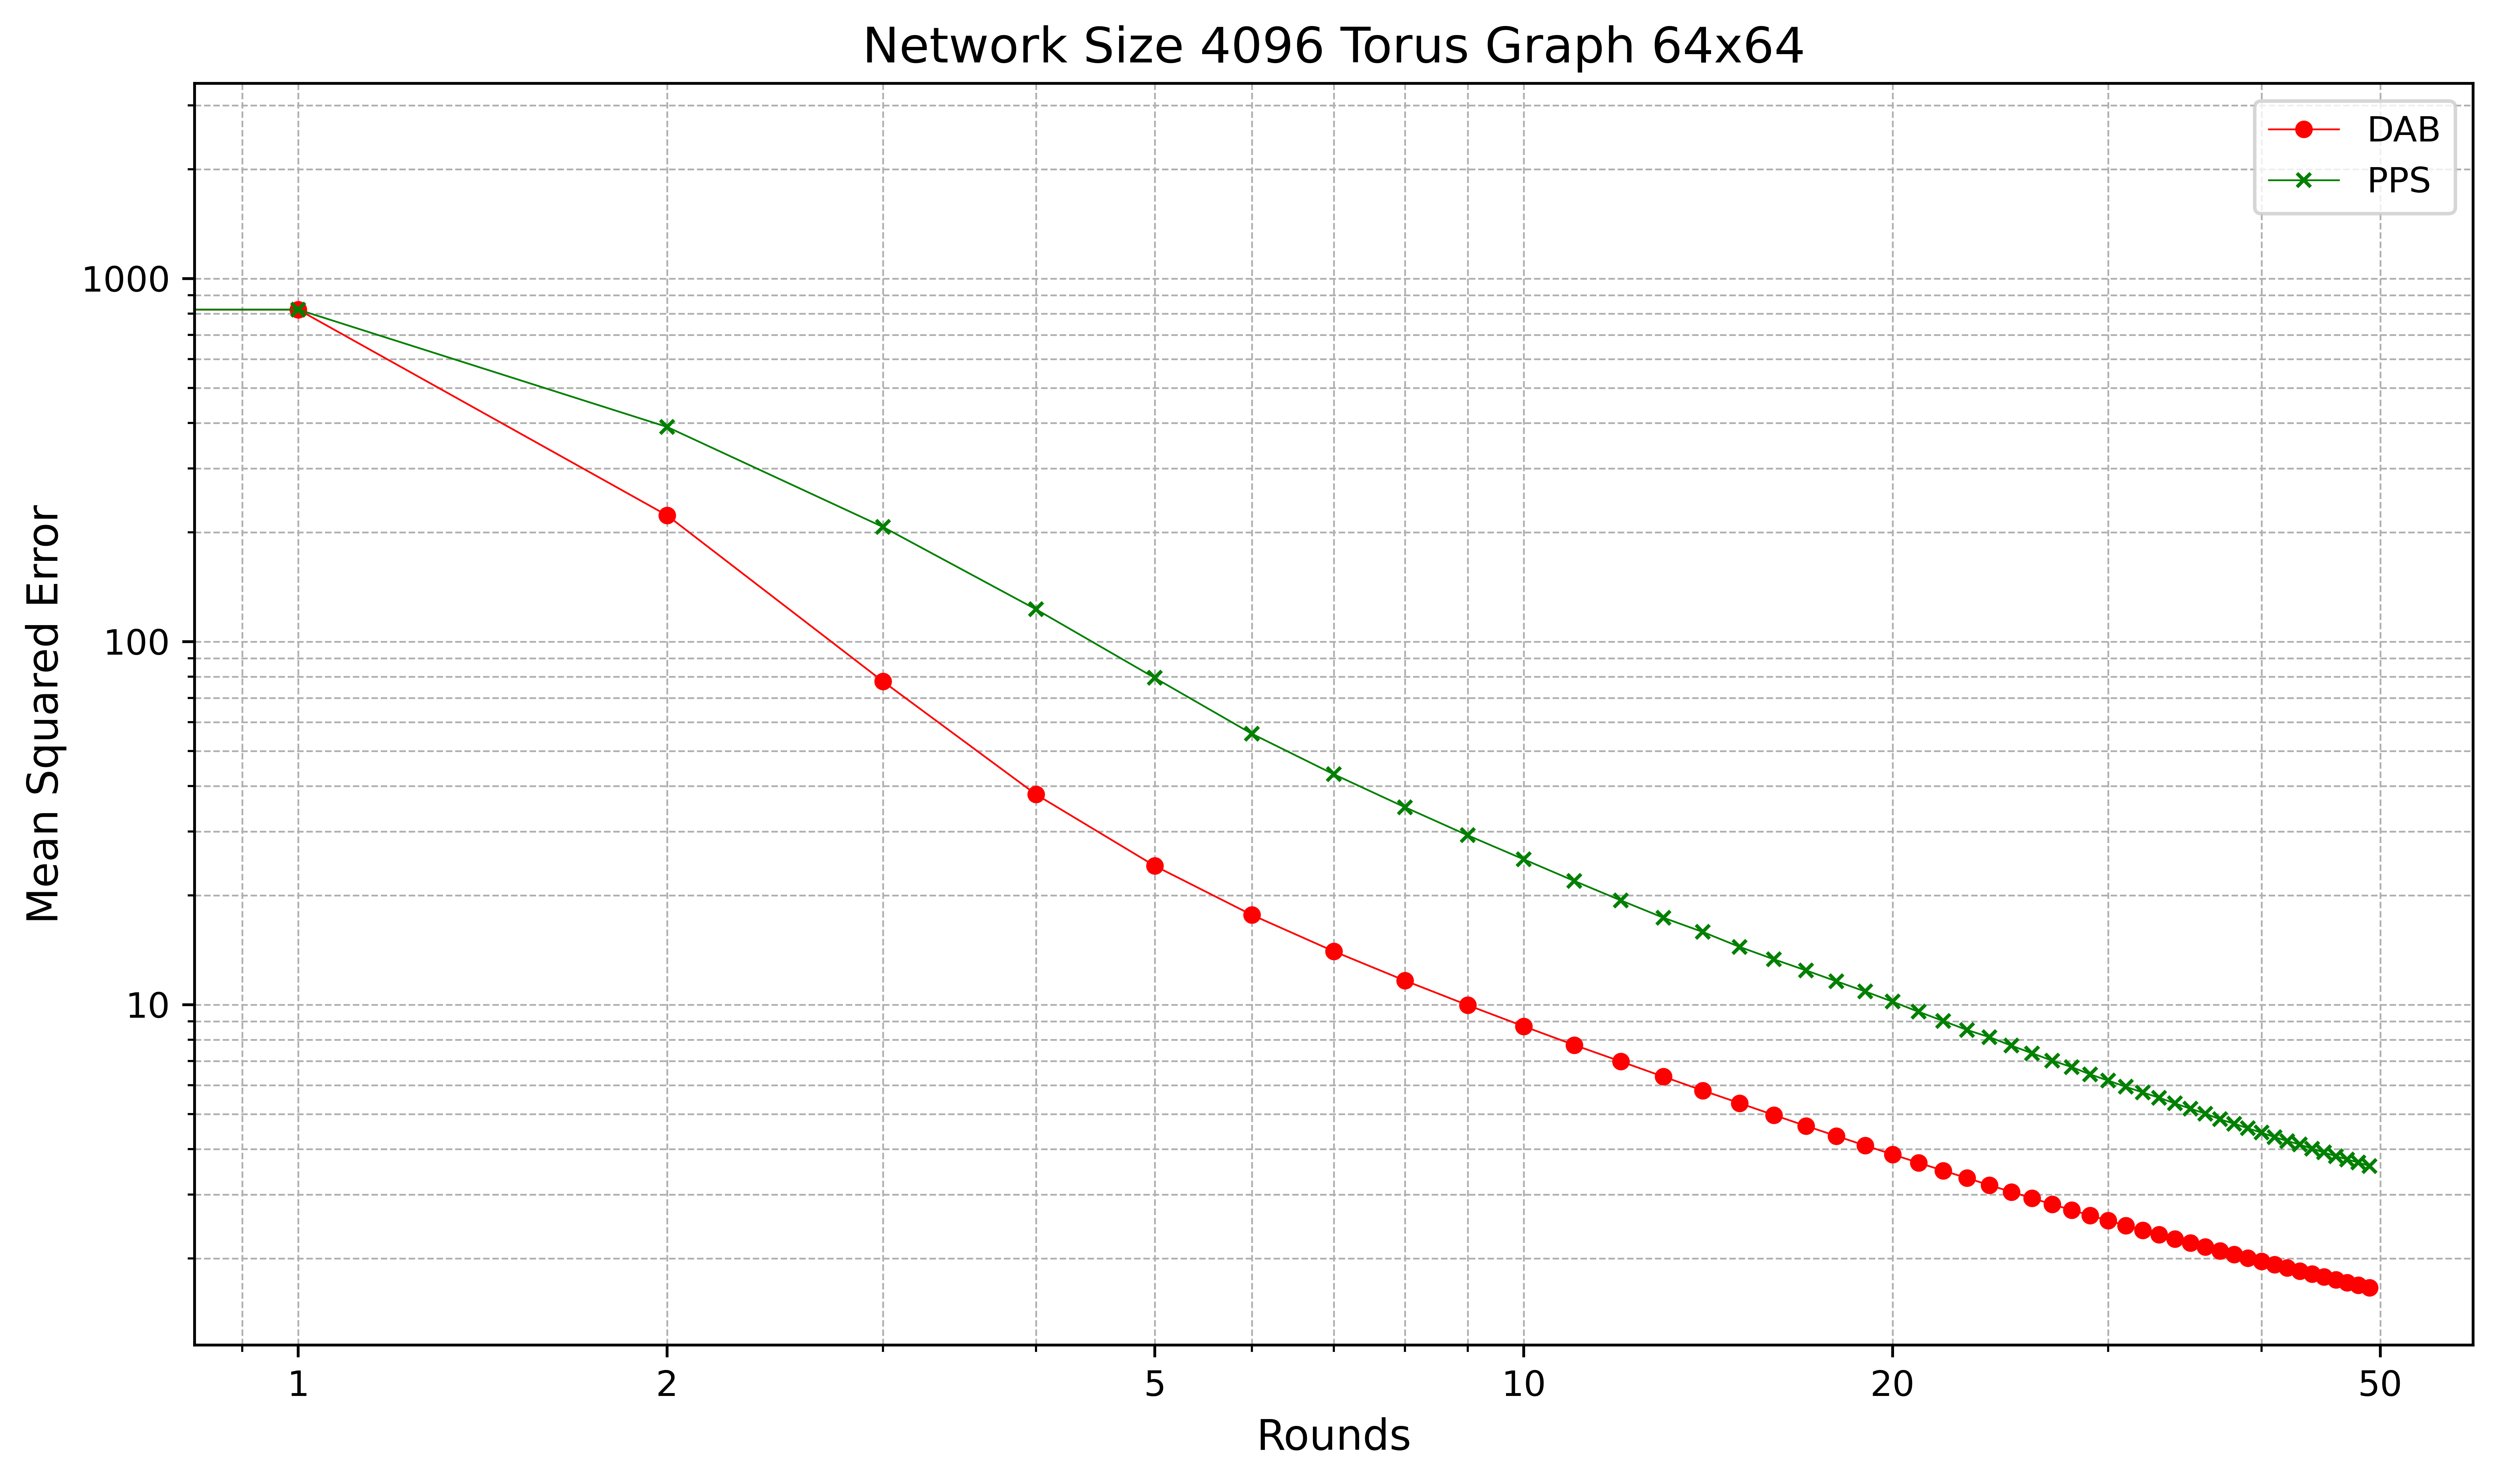
\includegraphics[scale=0.5]{figures/torusGridGraphSimulations/DAB_vs_PPS_TG_r50_n4096.png}
    \caption{Torus grid graph: network size $2^{12}$}
    \label{fig:4096torusGraph}
\end{figure}

\subsection{Network Sizes 2\textsuperscript{14}}
\textbf{Figures}: \ref{fig:16384torusGraph}, \ref{fig:32x512torusGraph}, \ref{fig:512x32torusGraph}\\
\textbf{Observations}: For the network size $2^{14}$ three different simulations were conducted using torus grid graphs with dimensions $2^{7} \times 2^{7}$, $2^{5} \times 2^{9}$ and $2^{9} \times 2^{5}$. The purpose was to demonstrate that varying the width and height of the torus graph does not significantly affect the behavior of the load-balancing protocols, since there is no change in connectivity (still a regular graph with degree 4). Many load-balancing protocols operate relying on local information, such as the state of neighboring nodes. In a torus grid, the local neighborhood of each node remains mostly consistent for the most nodes because the structure is highly regular and symmetric (for the edge nodes - the nodes with the wrap around edges - and their neighbors the neighborhood changes with change of the width and height). This consistency means that the protocol's behavior will be largely independent of the overall size of the graph as long as the local neighborhood does not change significantly. That is the reason why altering width and height of a torus graph does not alter the behavior of the protocols. In all three variations of the given network size, the DAB protocol outperforms the PPS protocol.\\
\begin{figure}[H]
    \centering
    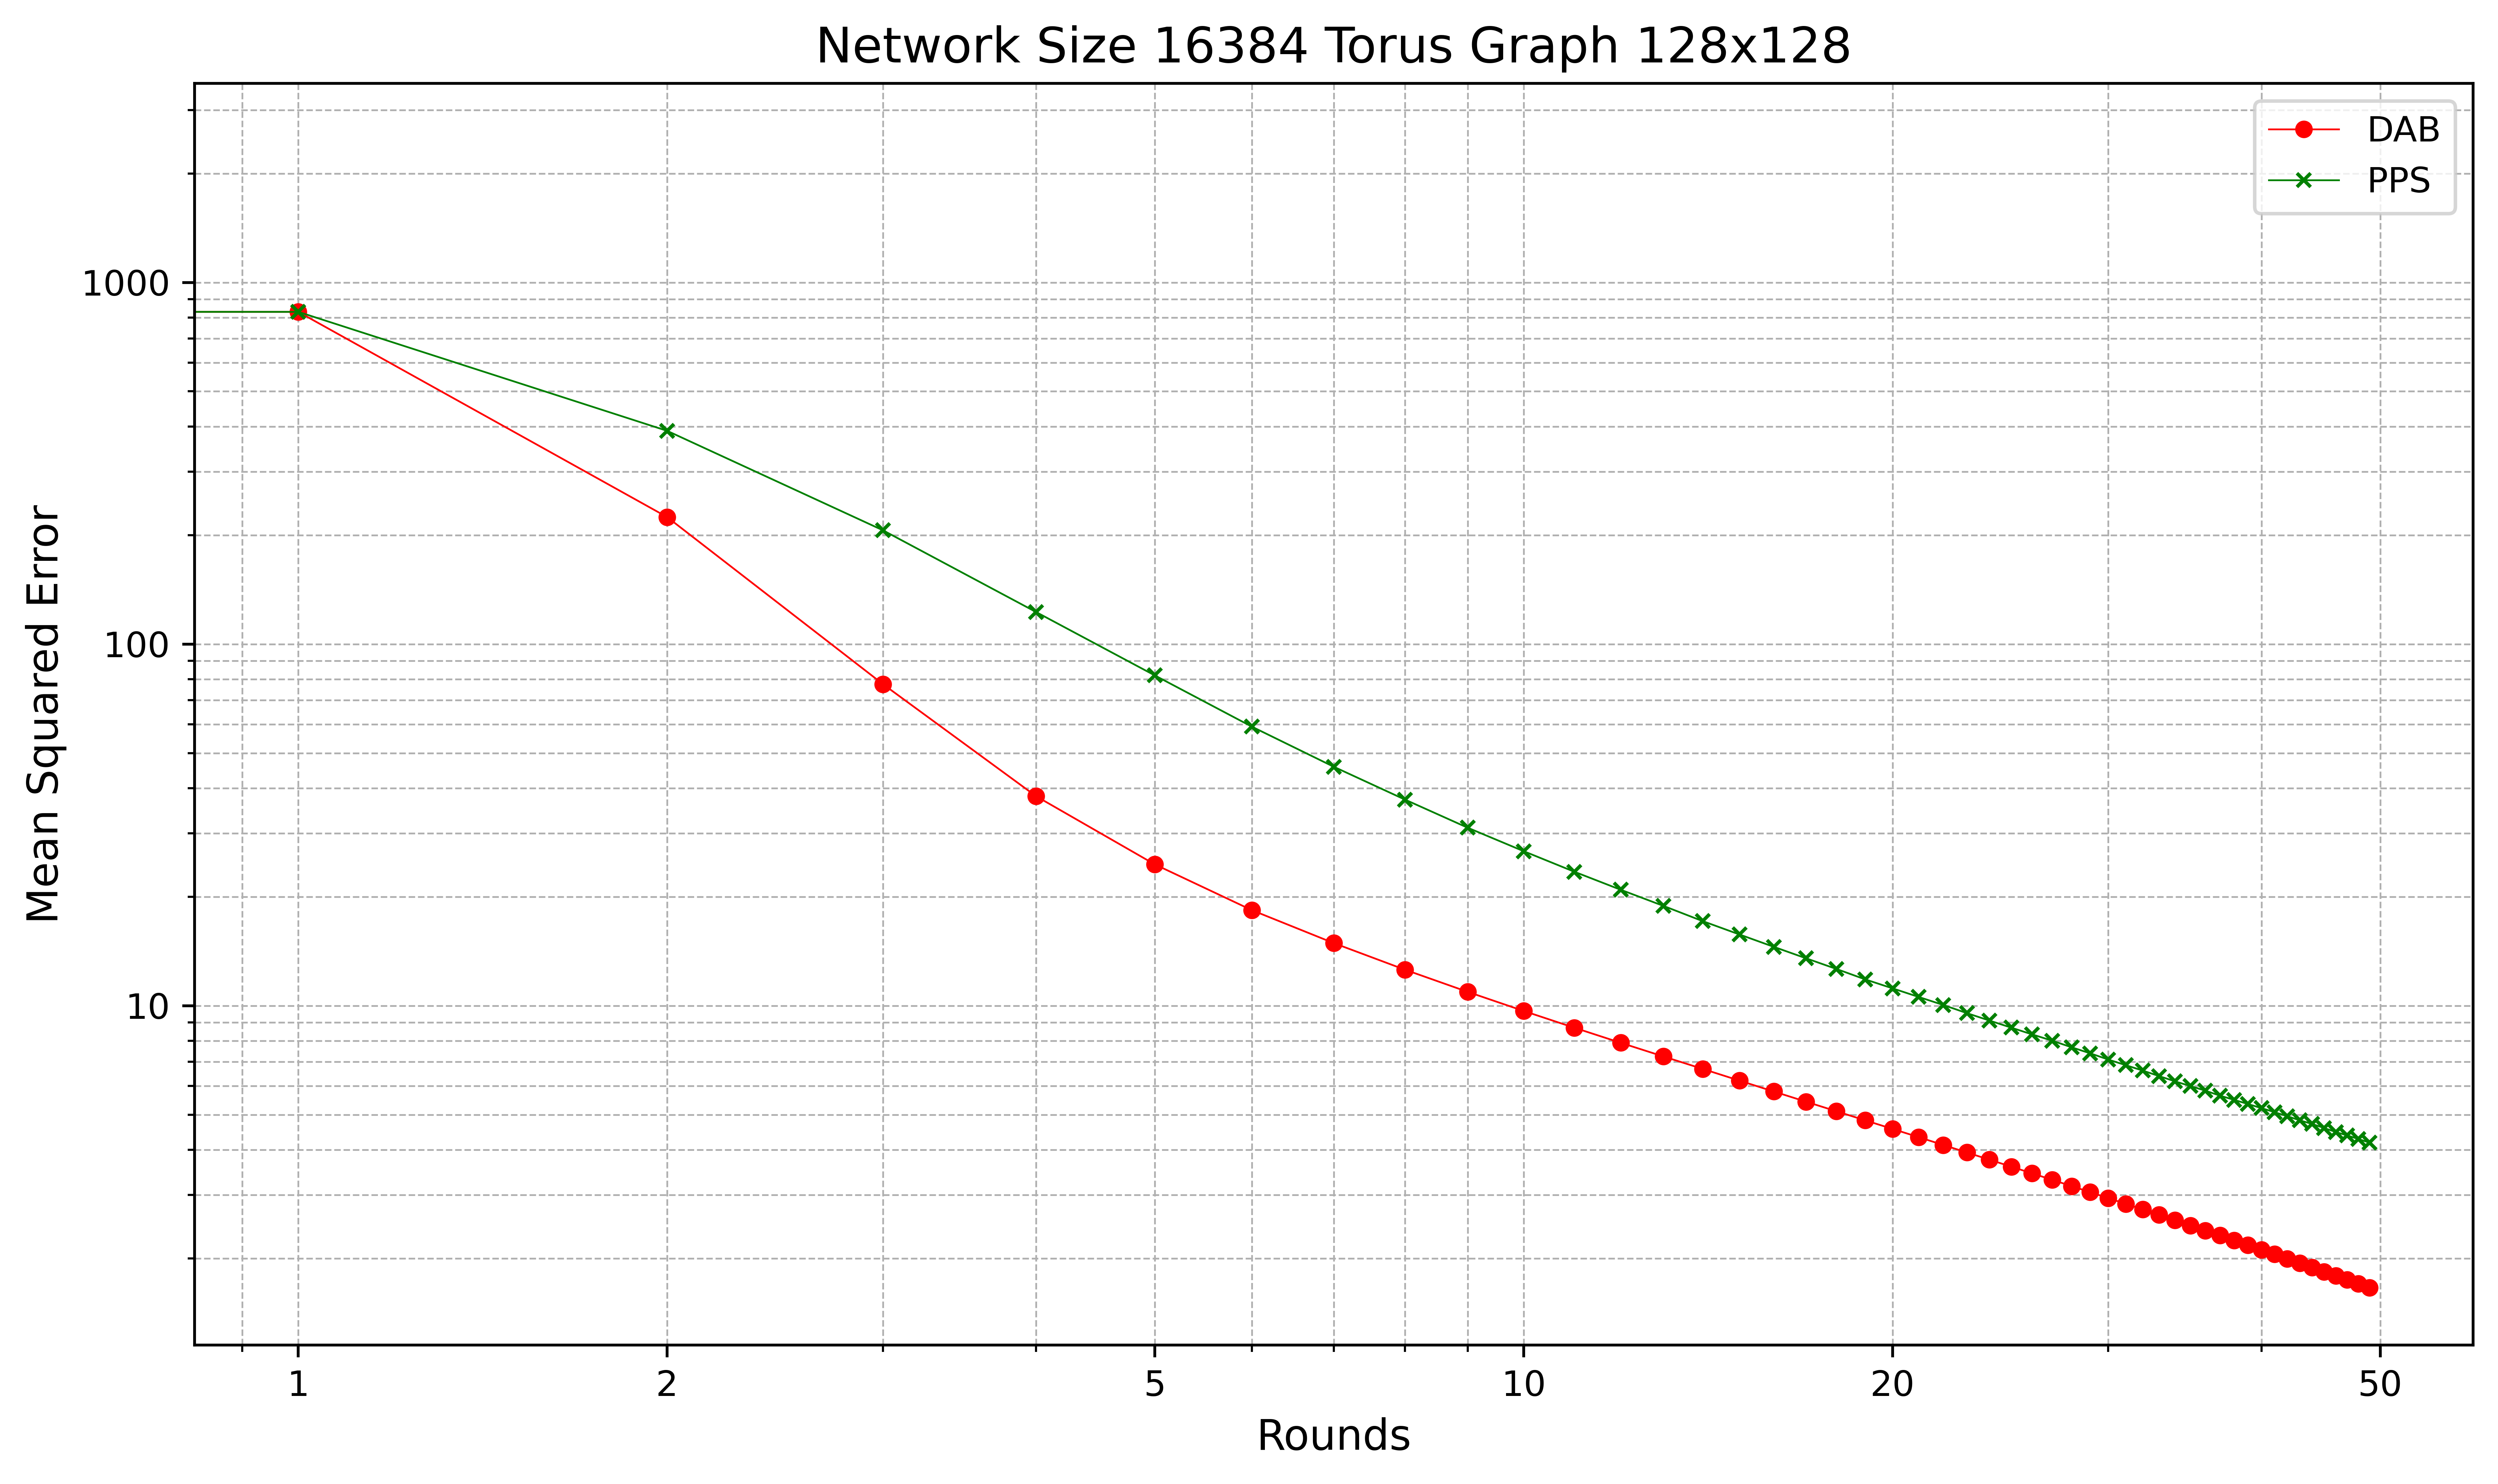
\includegraphics[scale=0.5]{figures/torusGridGraphSimulations/128x128/DAB_vs_PPS_TG_r50_n16384.png}
    \caption{Torus grid graph: network size $2^{14}$ $(128\times128)$}
    \label{fig:16384torusGraph}
\end{figure}

\begin{figure}[H]
    \centering
    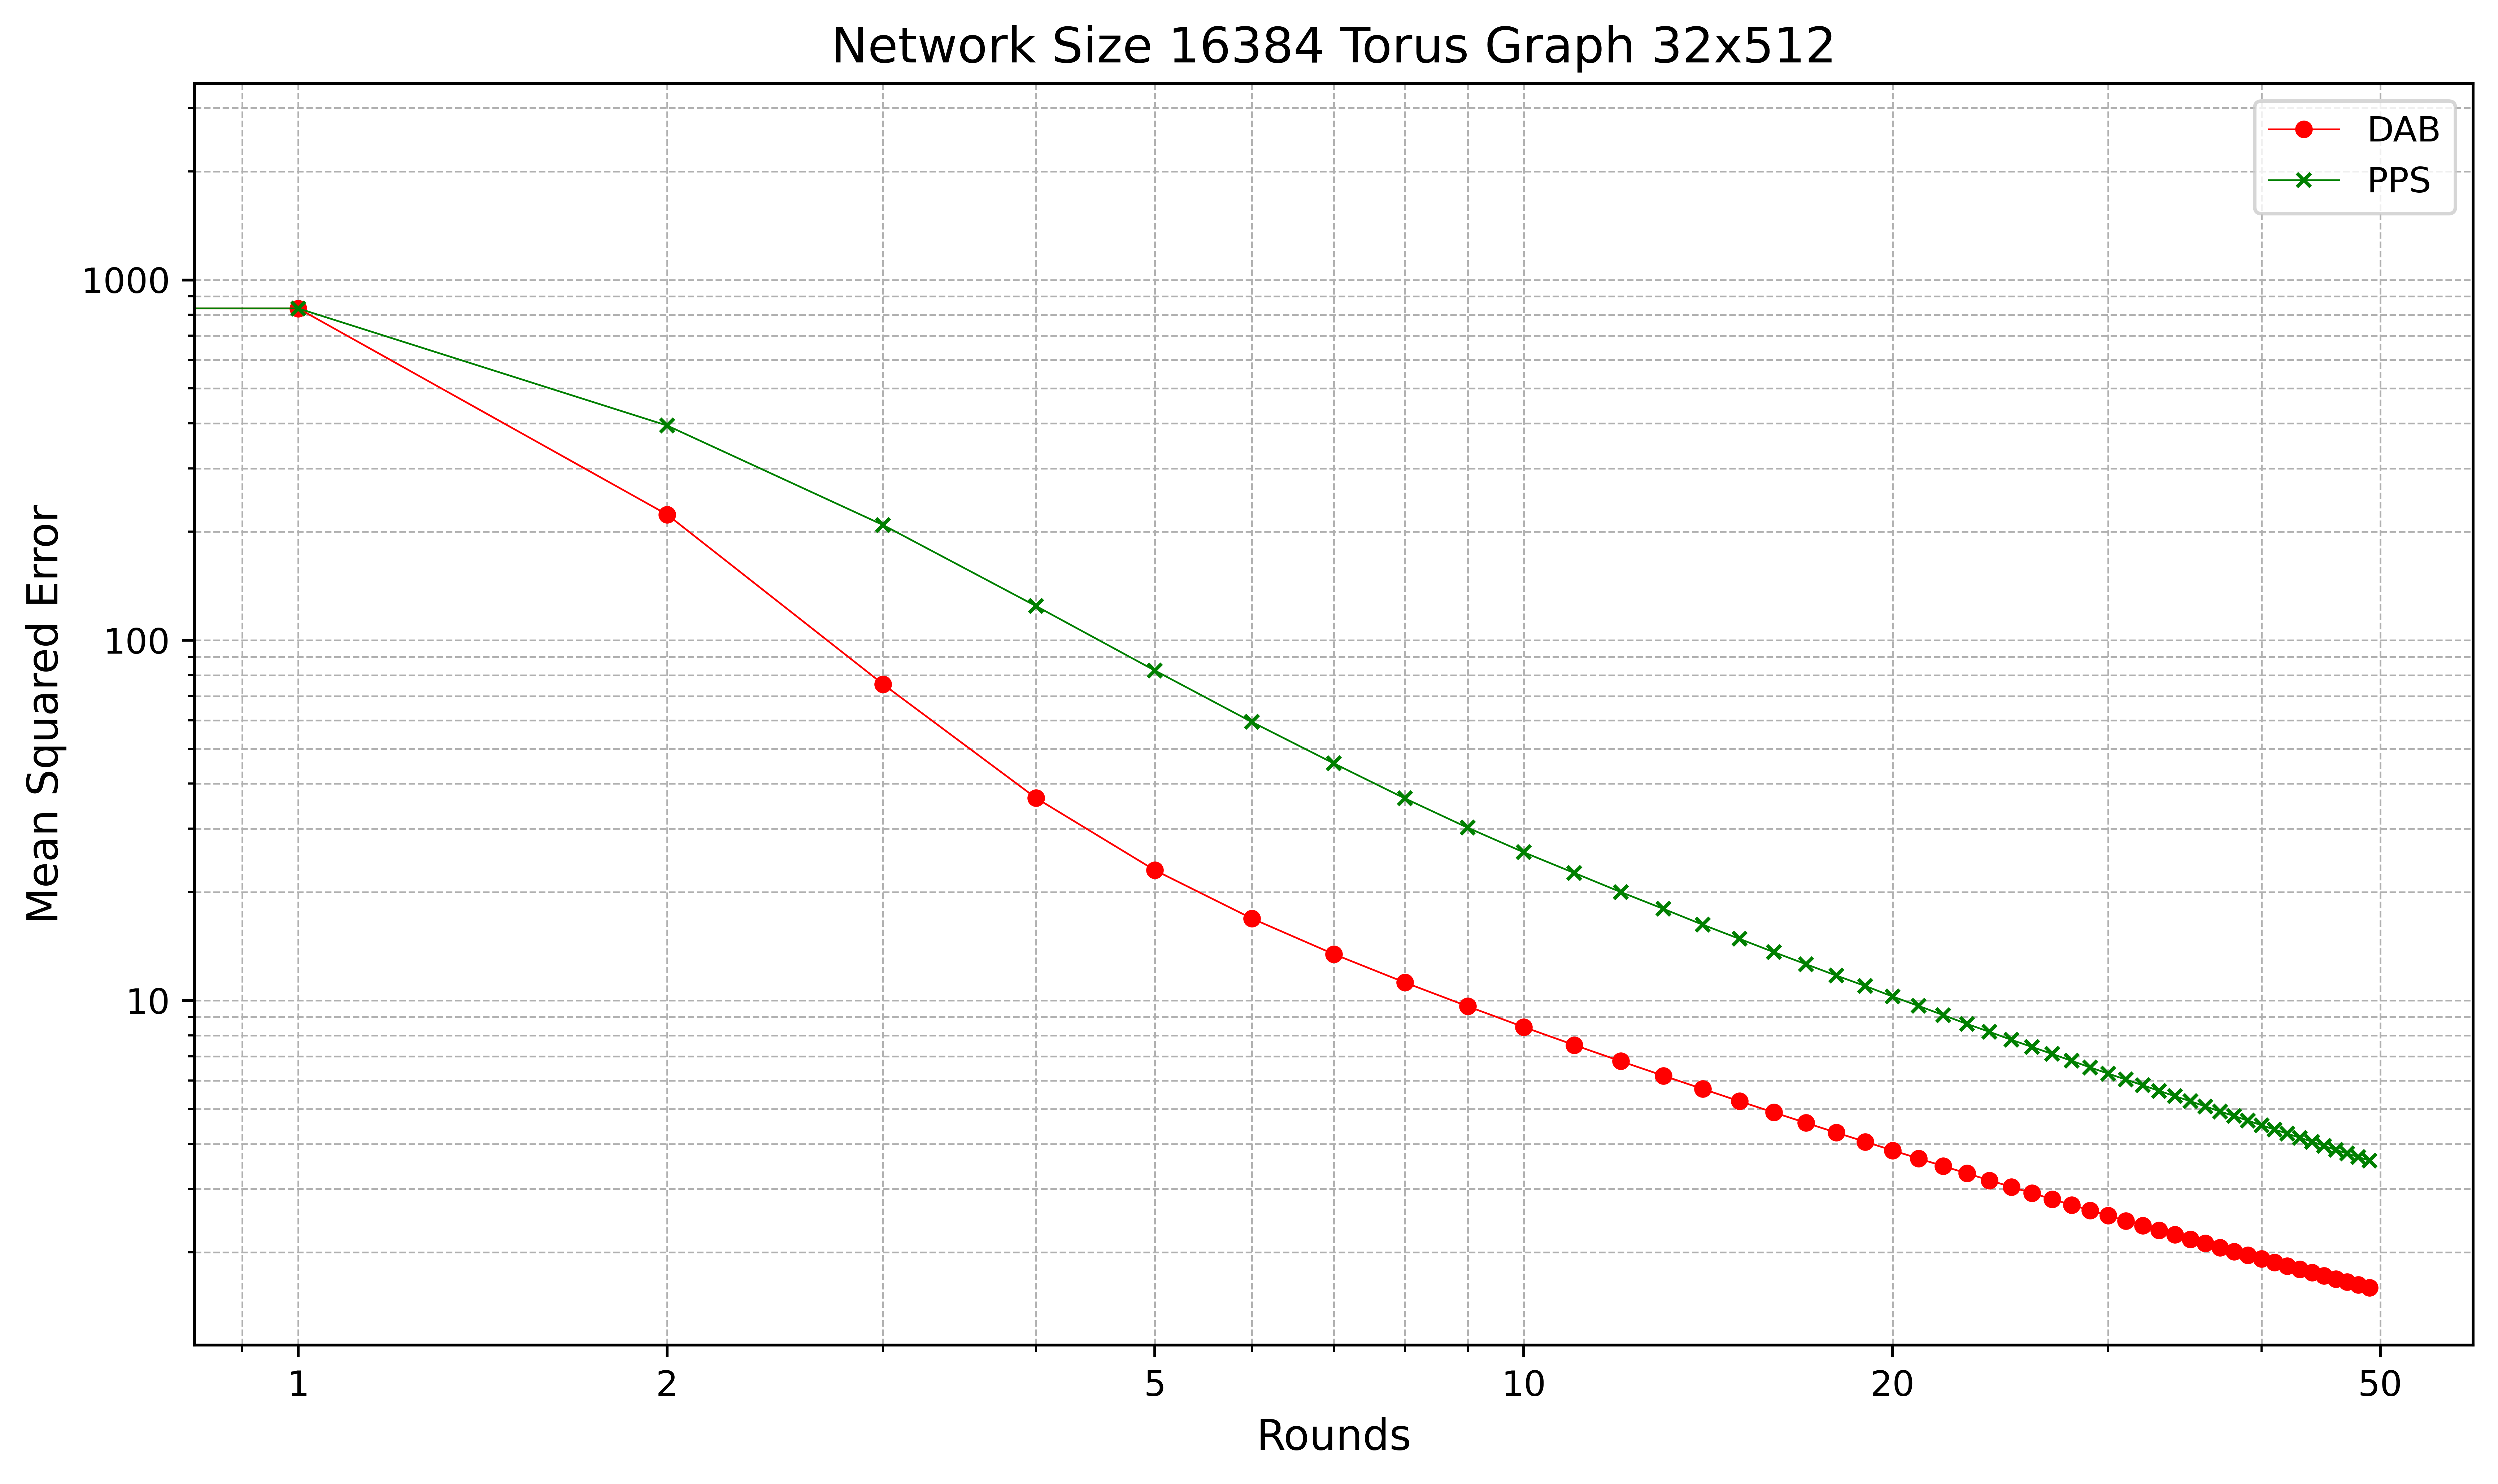
\includegraphics[scale=0.5]{figures/torusGridGraphSimulations/32x512/DAB_vs_PPS_TG_r50_n16384.png}
    \caption{Torus grid graph: network size $2^{14}$ $(32\times512)$}
    \label{fig:32x512torusGraph}
\end{figure}

\begin{figure}[H]
    \centering
    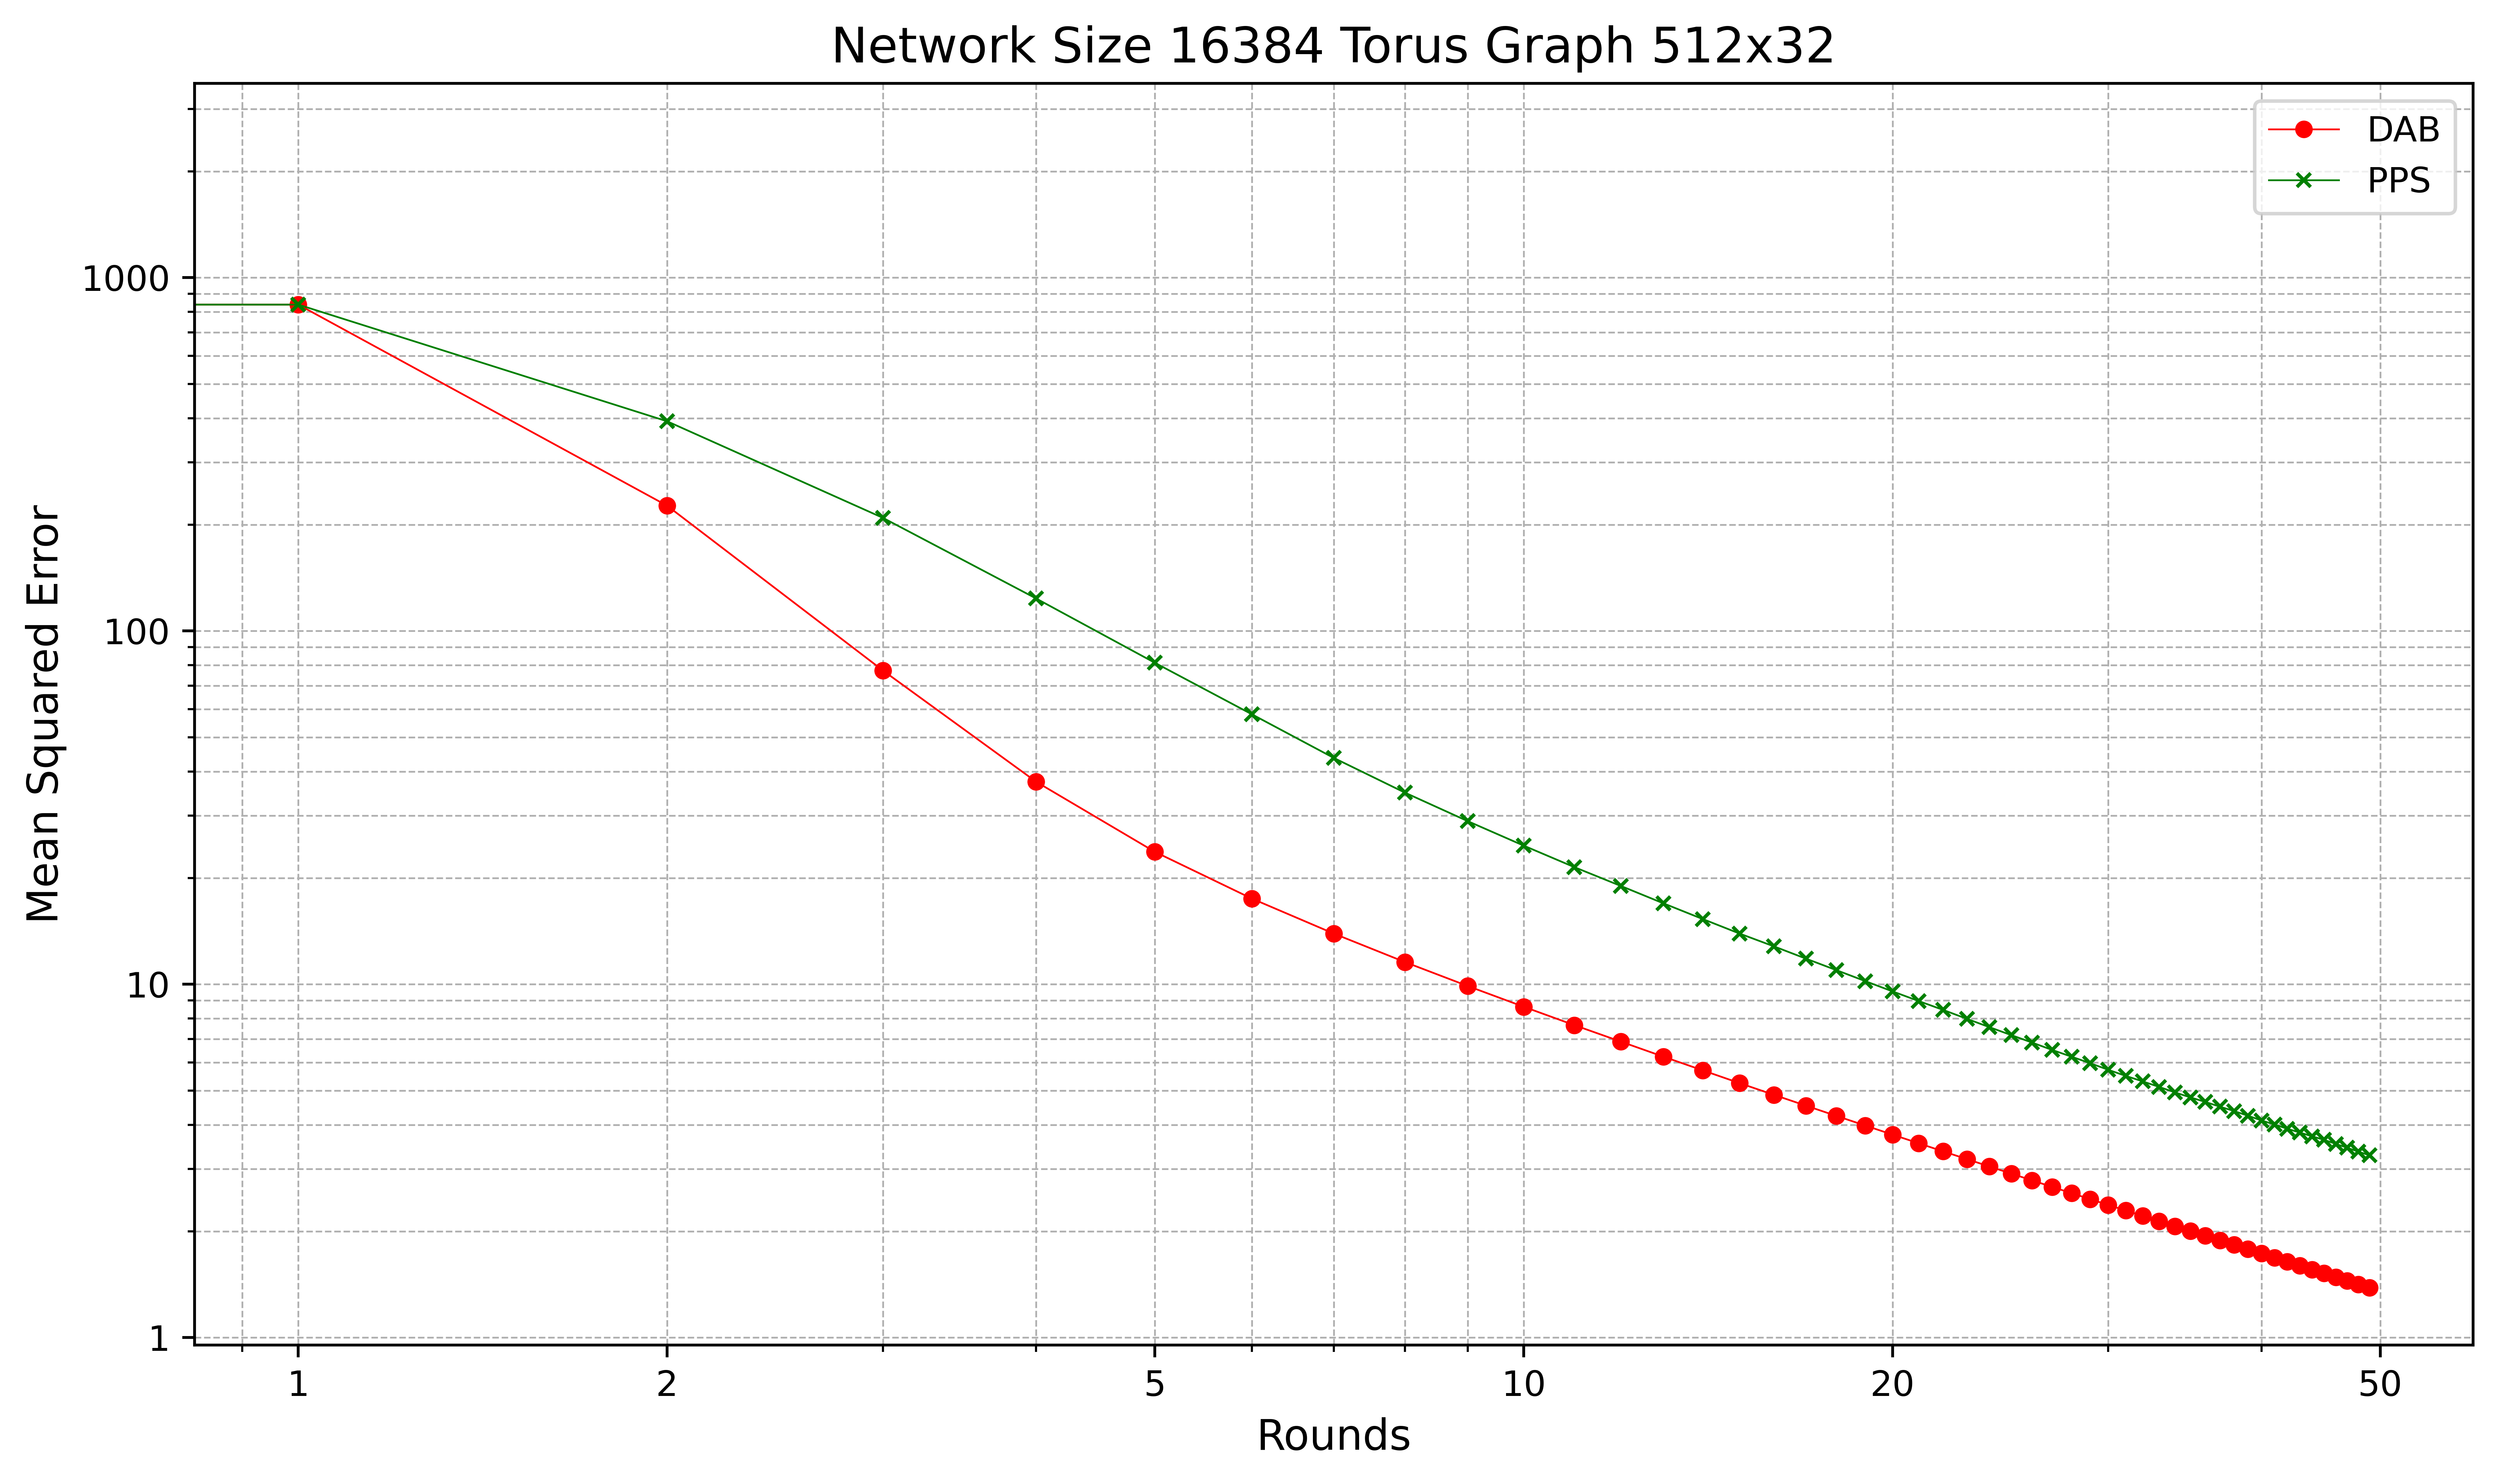
\includegraphics[scale=0.5]{figures/torusGridGraphSimulations/512x32/DAB_vs_PPS_TG_r50_n16384.png}
    \caption{Torus grid graph: network size $2^{14}$ $(512\times32)$}
    \label{fig:512x32torusGraph}
\end{figure}

\section{Ring of Cliques}
\textbf{The ring of cliques}: A $m \times n$ ring of cliques, consits of $m$ cliques, each containing $n$ nodes. These cliques are connected to form a ring structure. To create the ring, one edge from each clique is removed, and the endpoints of these removed edges are connected to form a regular graph \cite{Mahlmann2010}.  A $m \times n$ ring of cliques has $\left( m\times \left(\frac{n\times (n - 1)}{2}-1 \right) \right) +m$ edges. The connectivity of the graph increases with larger clique sizes and decreases with smaller clique sizes.
\begin{figure}[H]
    \centering
    \scalebox{1}{\newcommand\single[2]{
    \foreach \x in {1,...,#2}{
            \pgfmathsetmacro{\ang}{360/#2}
            \pgfmathparse{(\x-1)*\ang}
            \node[draw,fill=blue,circle,inner sep=3pt] (#1-\x) at (\pgfmathresult:10cm) {};
        }
    \foreach \x [count=\xi from 1] in {2,4}{
            \foreach \y in {2,4}{
                    \path (#1-\xi) edge[-] (#1-\y);
                    \path (#1-3) edge[-] (#1-\y);
                }
        }
}

\begin{tikzpicture}
    \begin{scope}[local bounding box=scope1]
    \end{scope}
    \foreach \s[count=\si from 0] in {0,90,...,360}{
            \begin{scope}[shift={($(scope1) +(\s:2)$)}, scale=0.1,rotate=\s+90]
                \single{\si}{4};
            \end{scope}
        }
    \foreach \i/\j in {1/2,2/3,3/4,4/1}
    \draw (\i-1)--(\j-3);
\end{tikzpicture}}
    \caption{Ring of cliques: network size 16}
    \label{fig:ringofcliquesDemo}
\end{figure}

\subsection{Network sizes: 2\textsuperscript{4}, 2\textsuperscript{8} and 2\textsuperscript{12}}
\textbf{Figures}: \ref{fig:16ringOfCliques}, \ref{fig:256ringOfCliques}, \ref{fig:4096ringOfCliques}\\
\textbf{Observations}: For a $4\times4$ ring of clique DAB outperforms PPS. From the start, the DAB protocol balances the network more quickly, which is likely due to the smaller network size and lower connectivity. In this setup, each clique has a size of four, giving each node a degree of three, as shown in \hyperref[fig:ringofcliquesDemo]{figure} \ref{fig:ringofcliquesDemo}. For smaller connectivity we observed that the DAB usually performs better than the PPS protocol. As the clique size increases, the PPS protocol begins to catch up with the DAB protocol, as seen in \hyperref[fig:256ringOfCliques]{figure} \ref{fig:256ringOfCliques} and \hyperref[fig:4096ringOfCliques]{figure} \ref{fig:4096ringOfCliques}.

For a $16\times16$ ring of cliques, PPS initially reduces the error of its network more quickly, but after round 9, the DAB catches up and ultimately reduces the error of the network faster. By round 50, the DAB-balanced network has an error of 14.31, while the PPS-balanced network has an error of 46.81 A similar observation can be made for the simulation for the $64 \times 64$ ring of cliques \ref{fig:4096ringOfCliques}. Again, the DAB catches up to the PPS protocol, resulting in a lower error of the network in round 50. However, the final errors at round 50 are closer to each other. This can be explained by the increased clique size in this simulation, which enhances the graph's connectivity. With larger network sizes and particularly with larger clique sizes, the MSE decreases more rapidly due to the higher number of messages being exchanged within the network \cite{nugroho2023PushPullSumDataAg}.

The DAB curve starts with a steep decline in MSE for network size of $2^{14}$, and its drop is more significant as rounds progress. The DAB protocol continues to reduce the MSE steadily, reaching very low error values by round 50. The PPS curve also starts with a rapid decline in MSE, but the descent is slower compared to DAB, especially in the later rounds. It seems like the PPS is converging, but at a much slower rate than DAB after reaching a certain threshold (round 6). For network sizes $2^{8}$ and $2^{12}$ the DAB curve starts with a very slow decline in MSE for the first 10-15 rounds. In the later rounds, DAB converges very effectively, bringing the MSE down to a lower value than the PPS by the end of round 50. PPS, in contrast, starts with a much faster decline in MSE from the very first round. It shows a steady and significant reduction in MSE. After round 10, PPS does not improve as much and remains mostly flat, maintaining its MSE at a low value, with only slight improvements in the later rounds (graph is stagnating).

\begin{figure}[H]
    \centering
    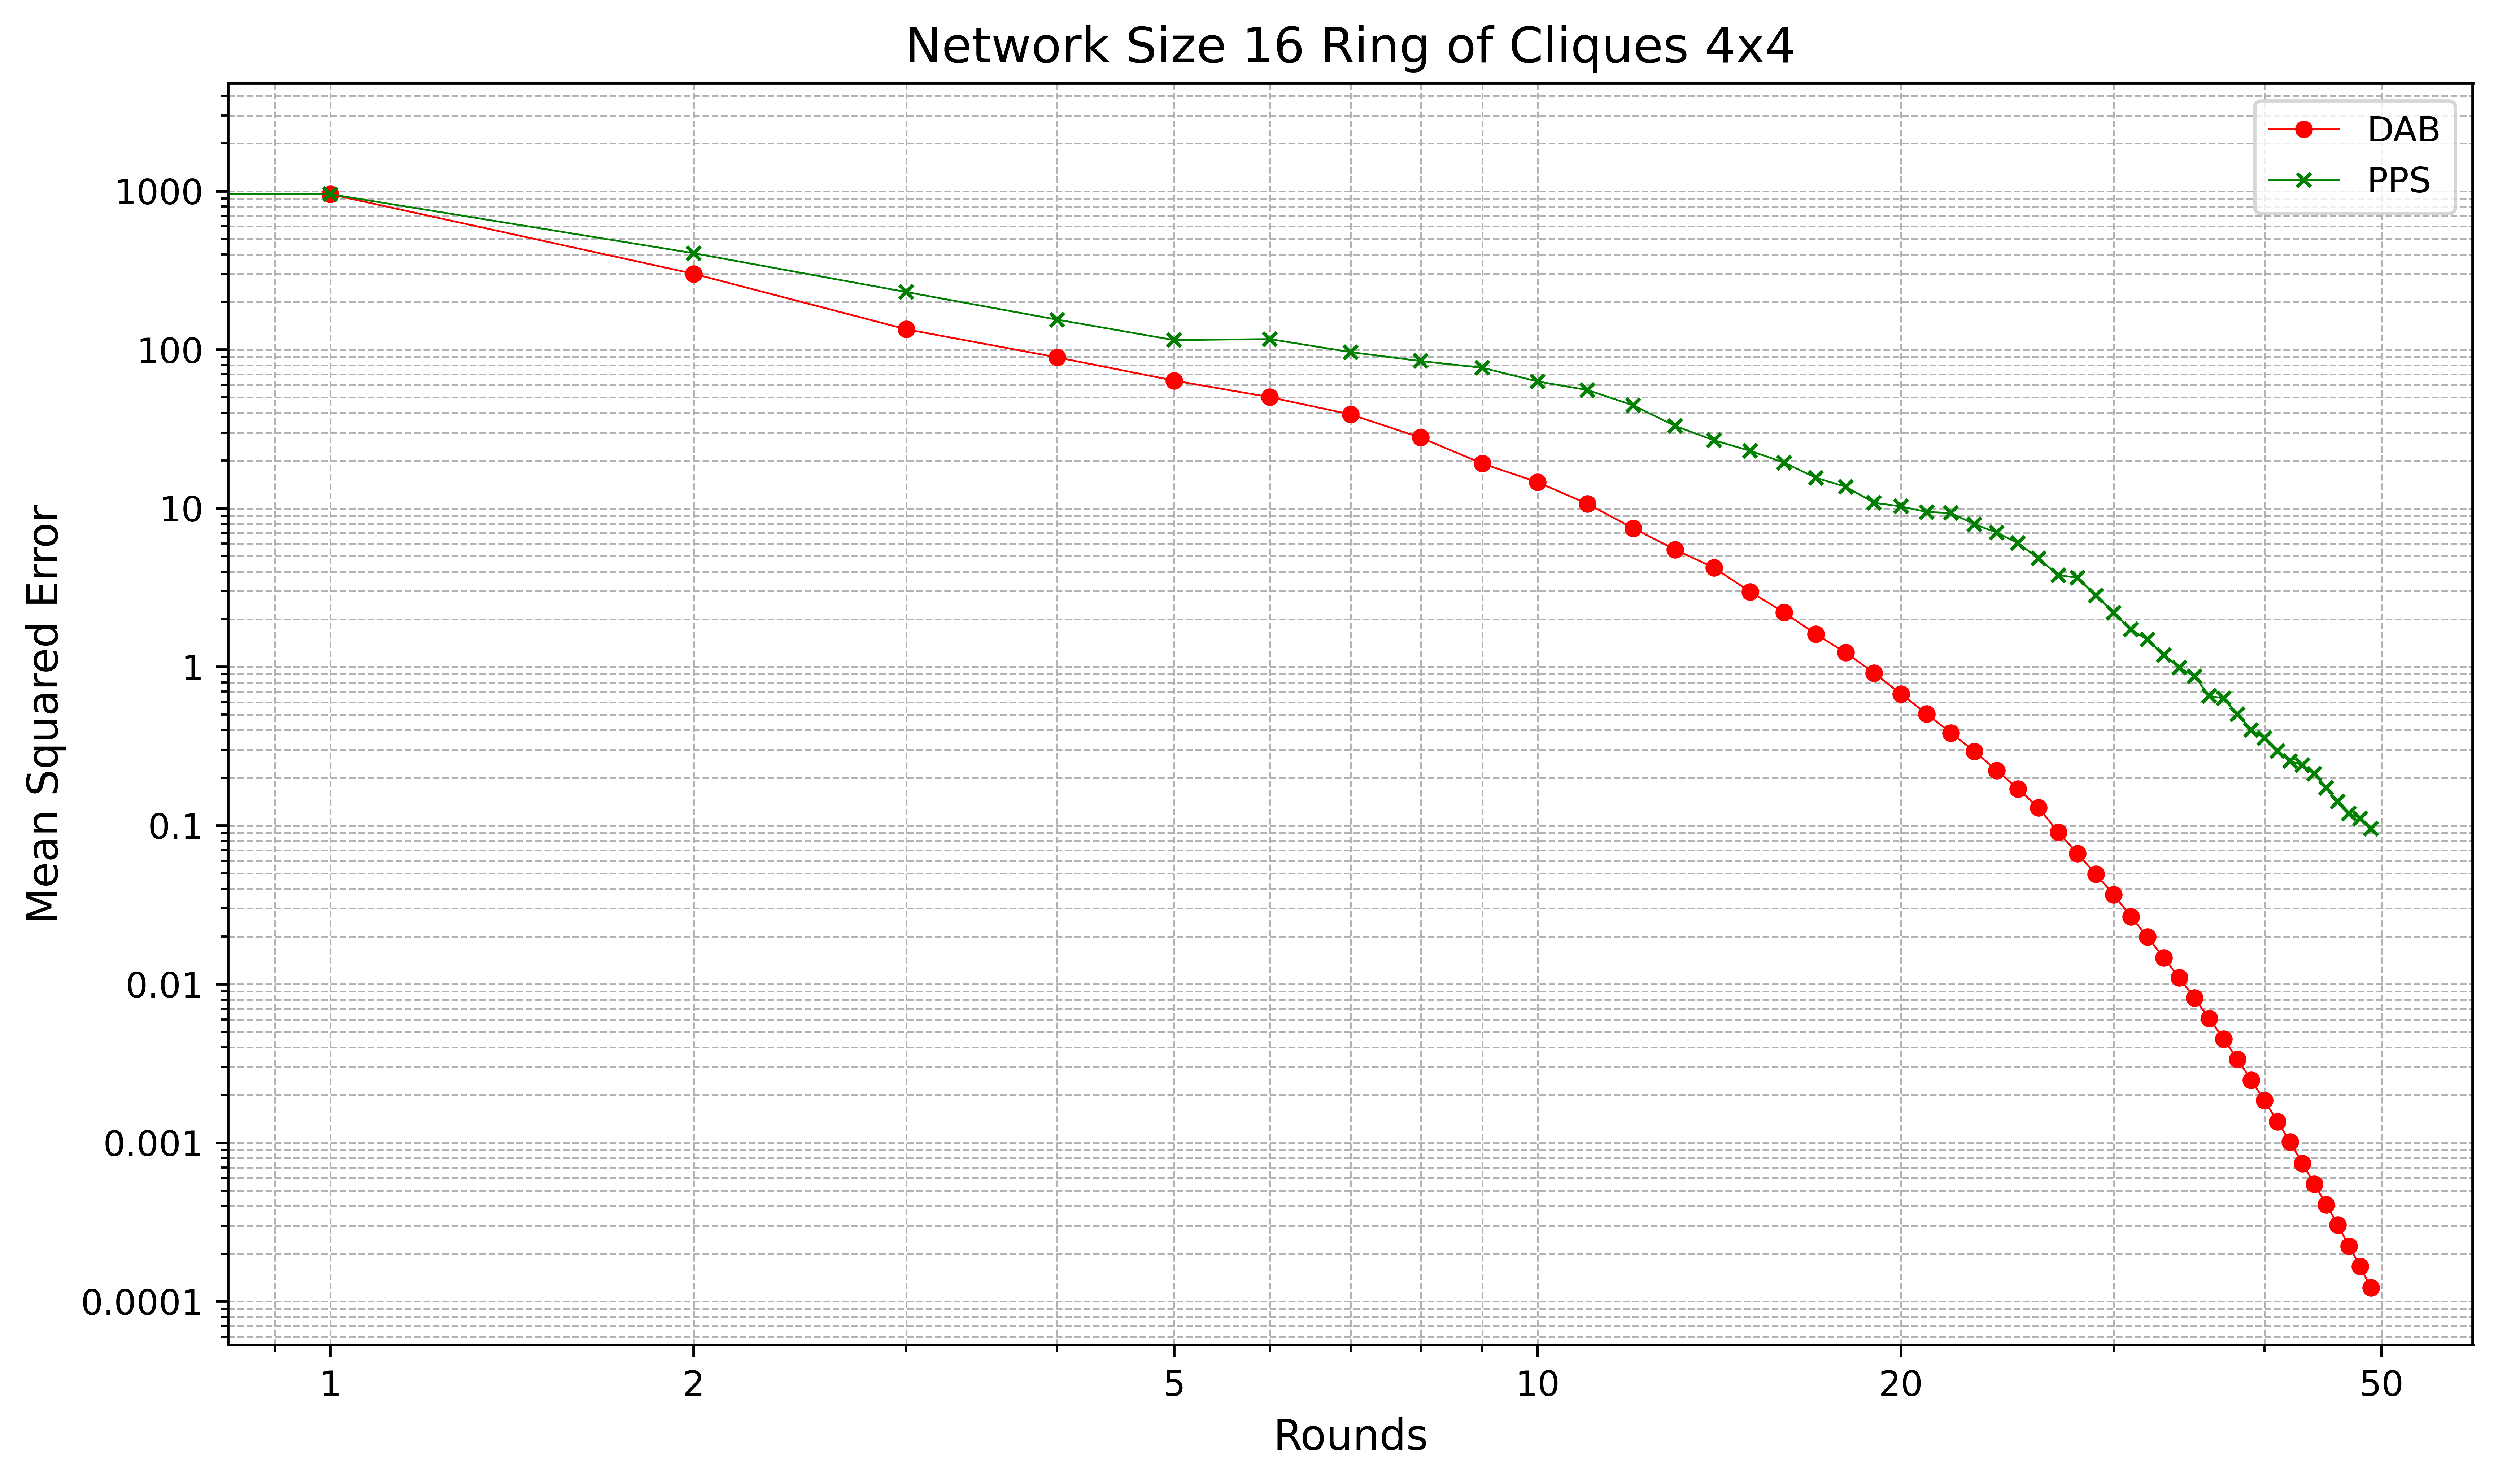
\includegraphics[scale=0.5]{figures/ringOfCliquesSimulations/DAB_vs_PPS_RoC_r50_n16.png}
    \caption{Ring of cliques: network size $2^{4}$ $(4\times4)$}
    \label{fig:16ringOfCliques}
\end{figure}

\begin{figure}[H]
    \centering
    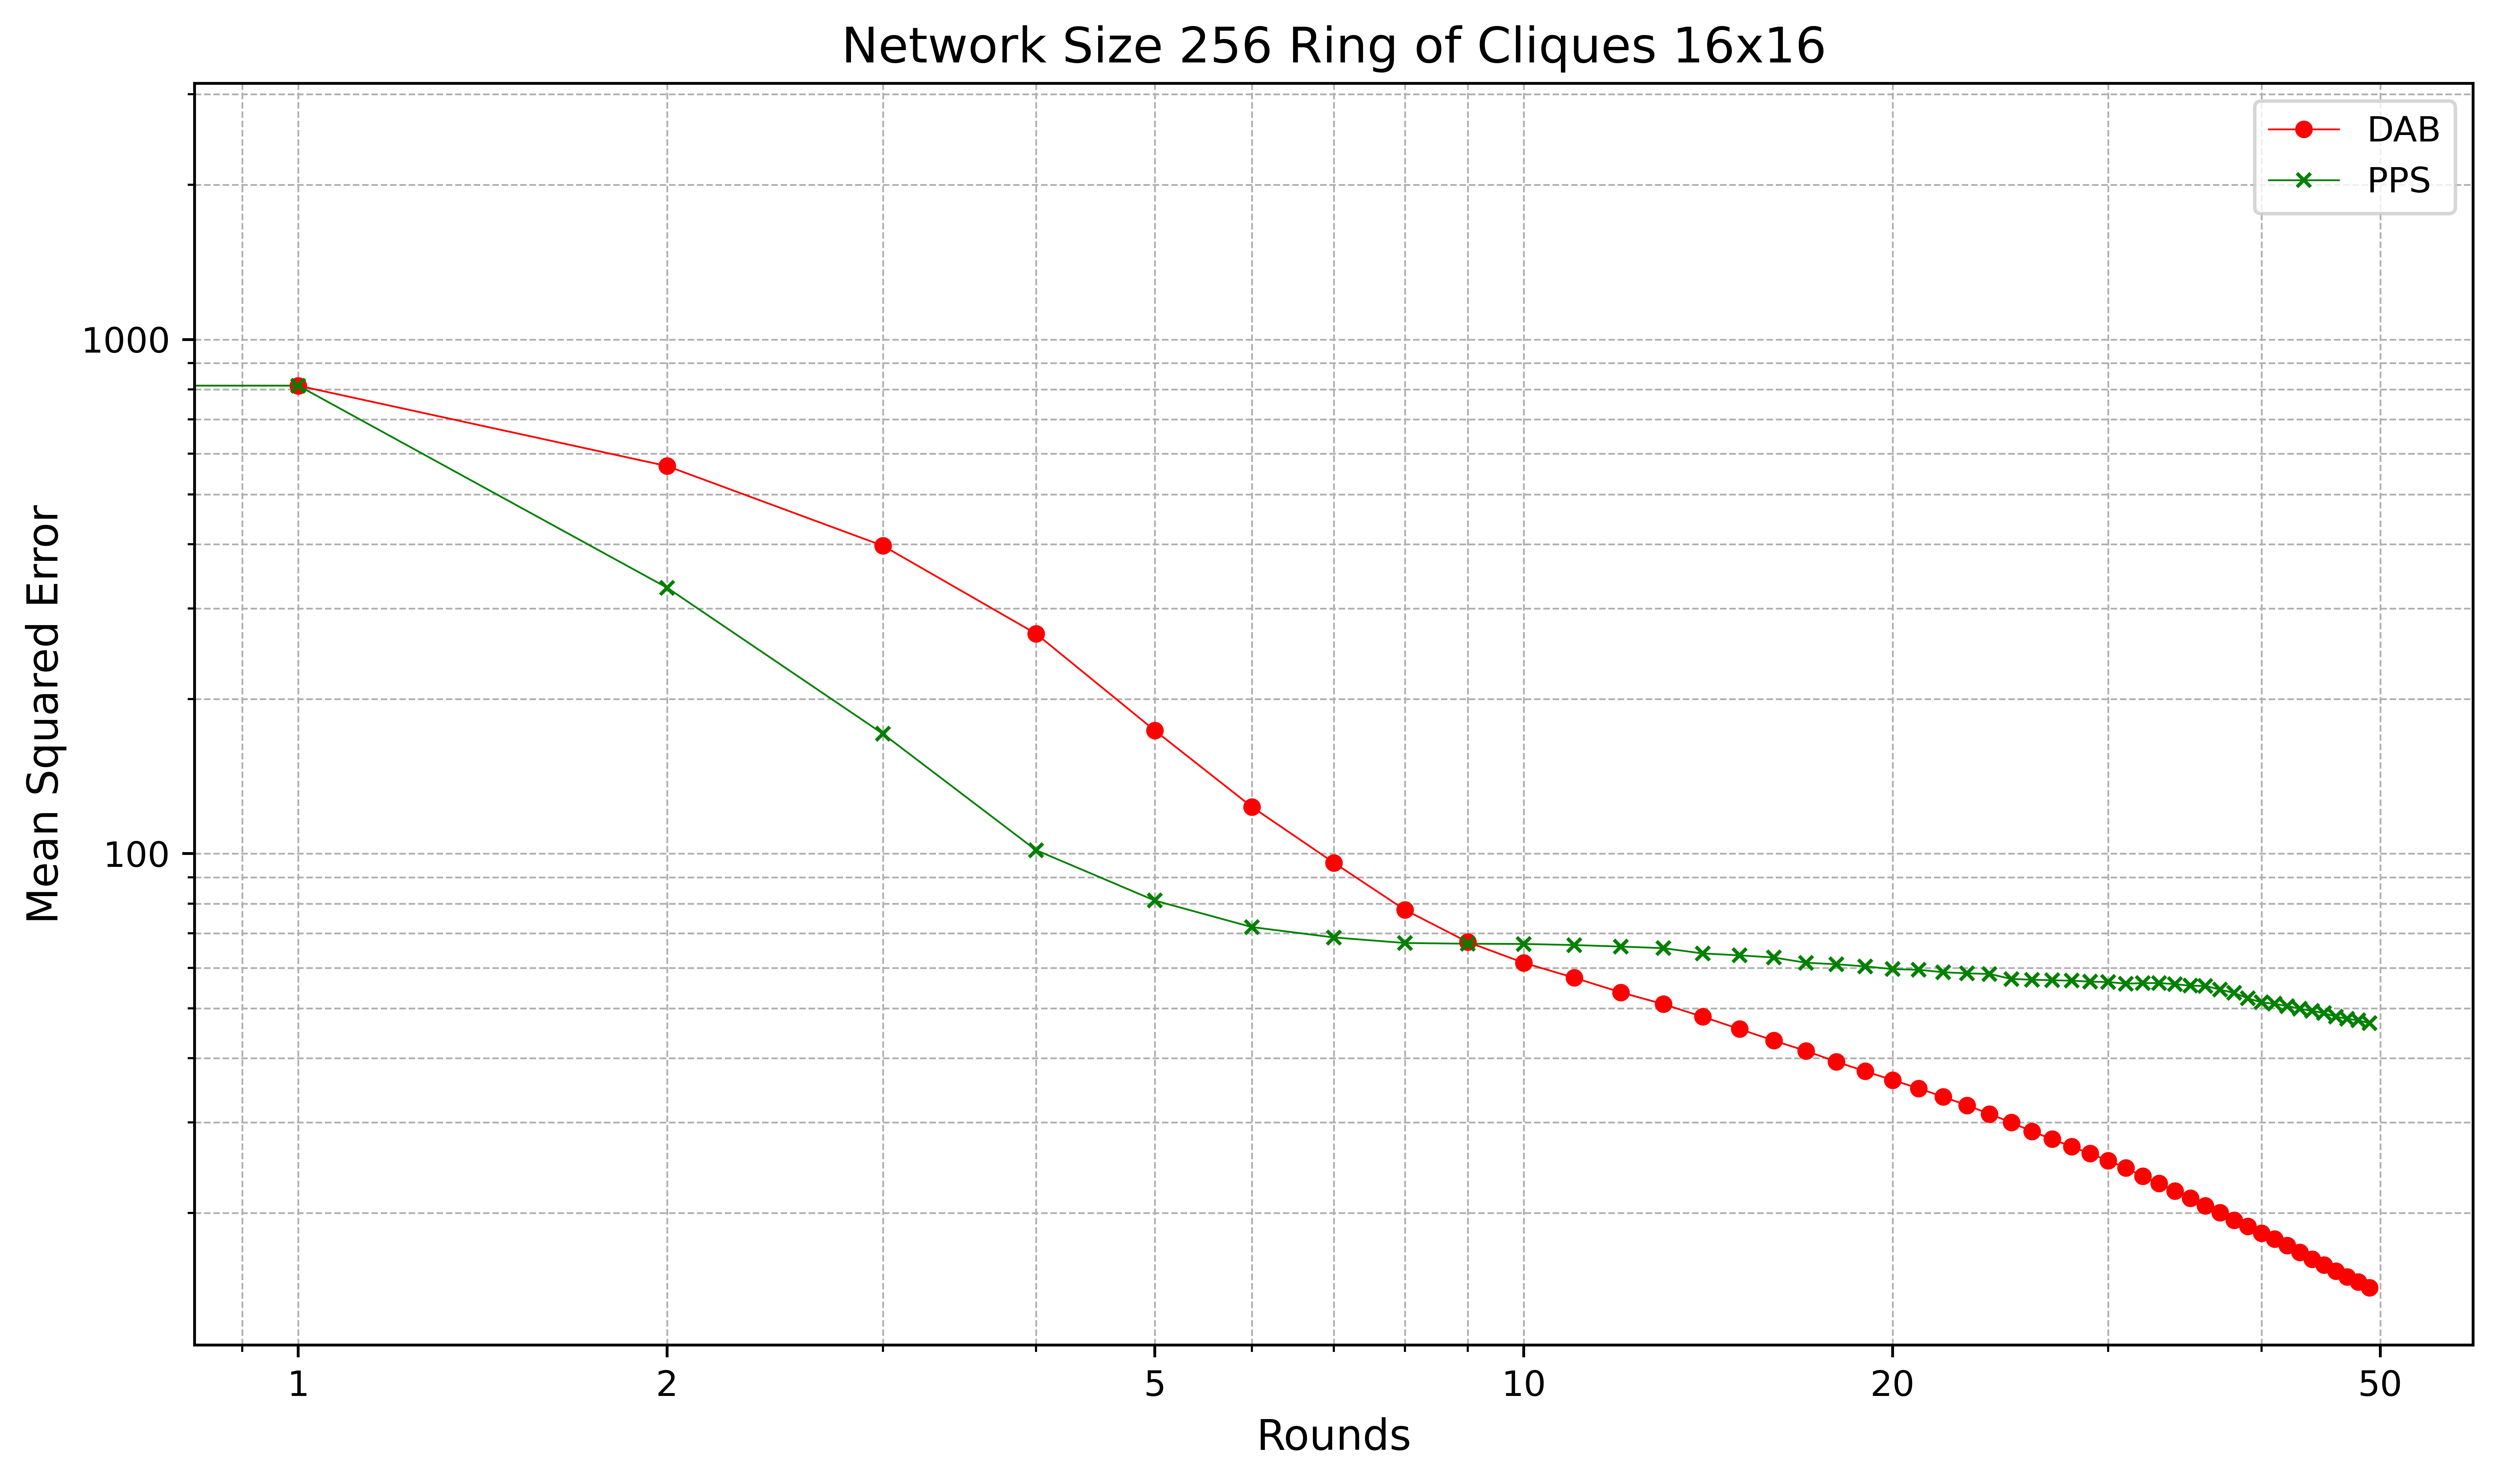
\includegraphics[scale=0.5]{figures/ringOfCliquesSimulations/DAB_vs_PPS_RoC_r50_n256.png}
    \caption{Ring of cliques: network size $2^{8}$ $(16\times16)$}
    \label{fig:256ringOfCliques}
\end{figure}

\begin{figure}[H]
    \centering
    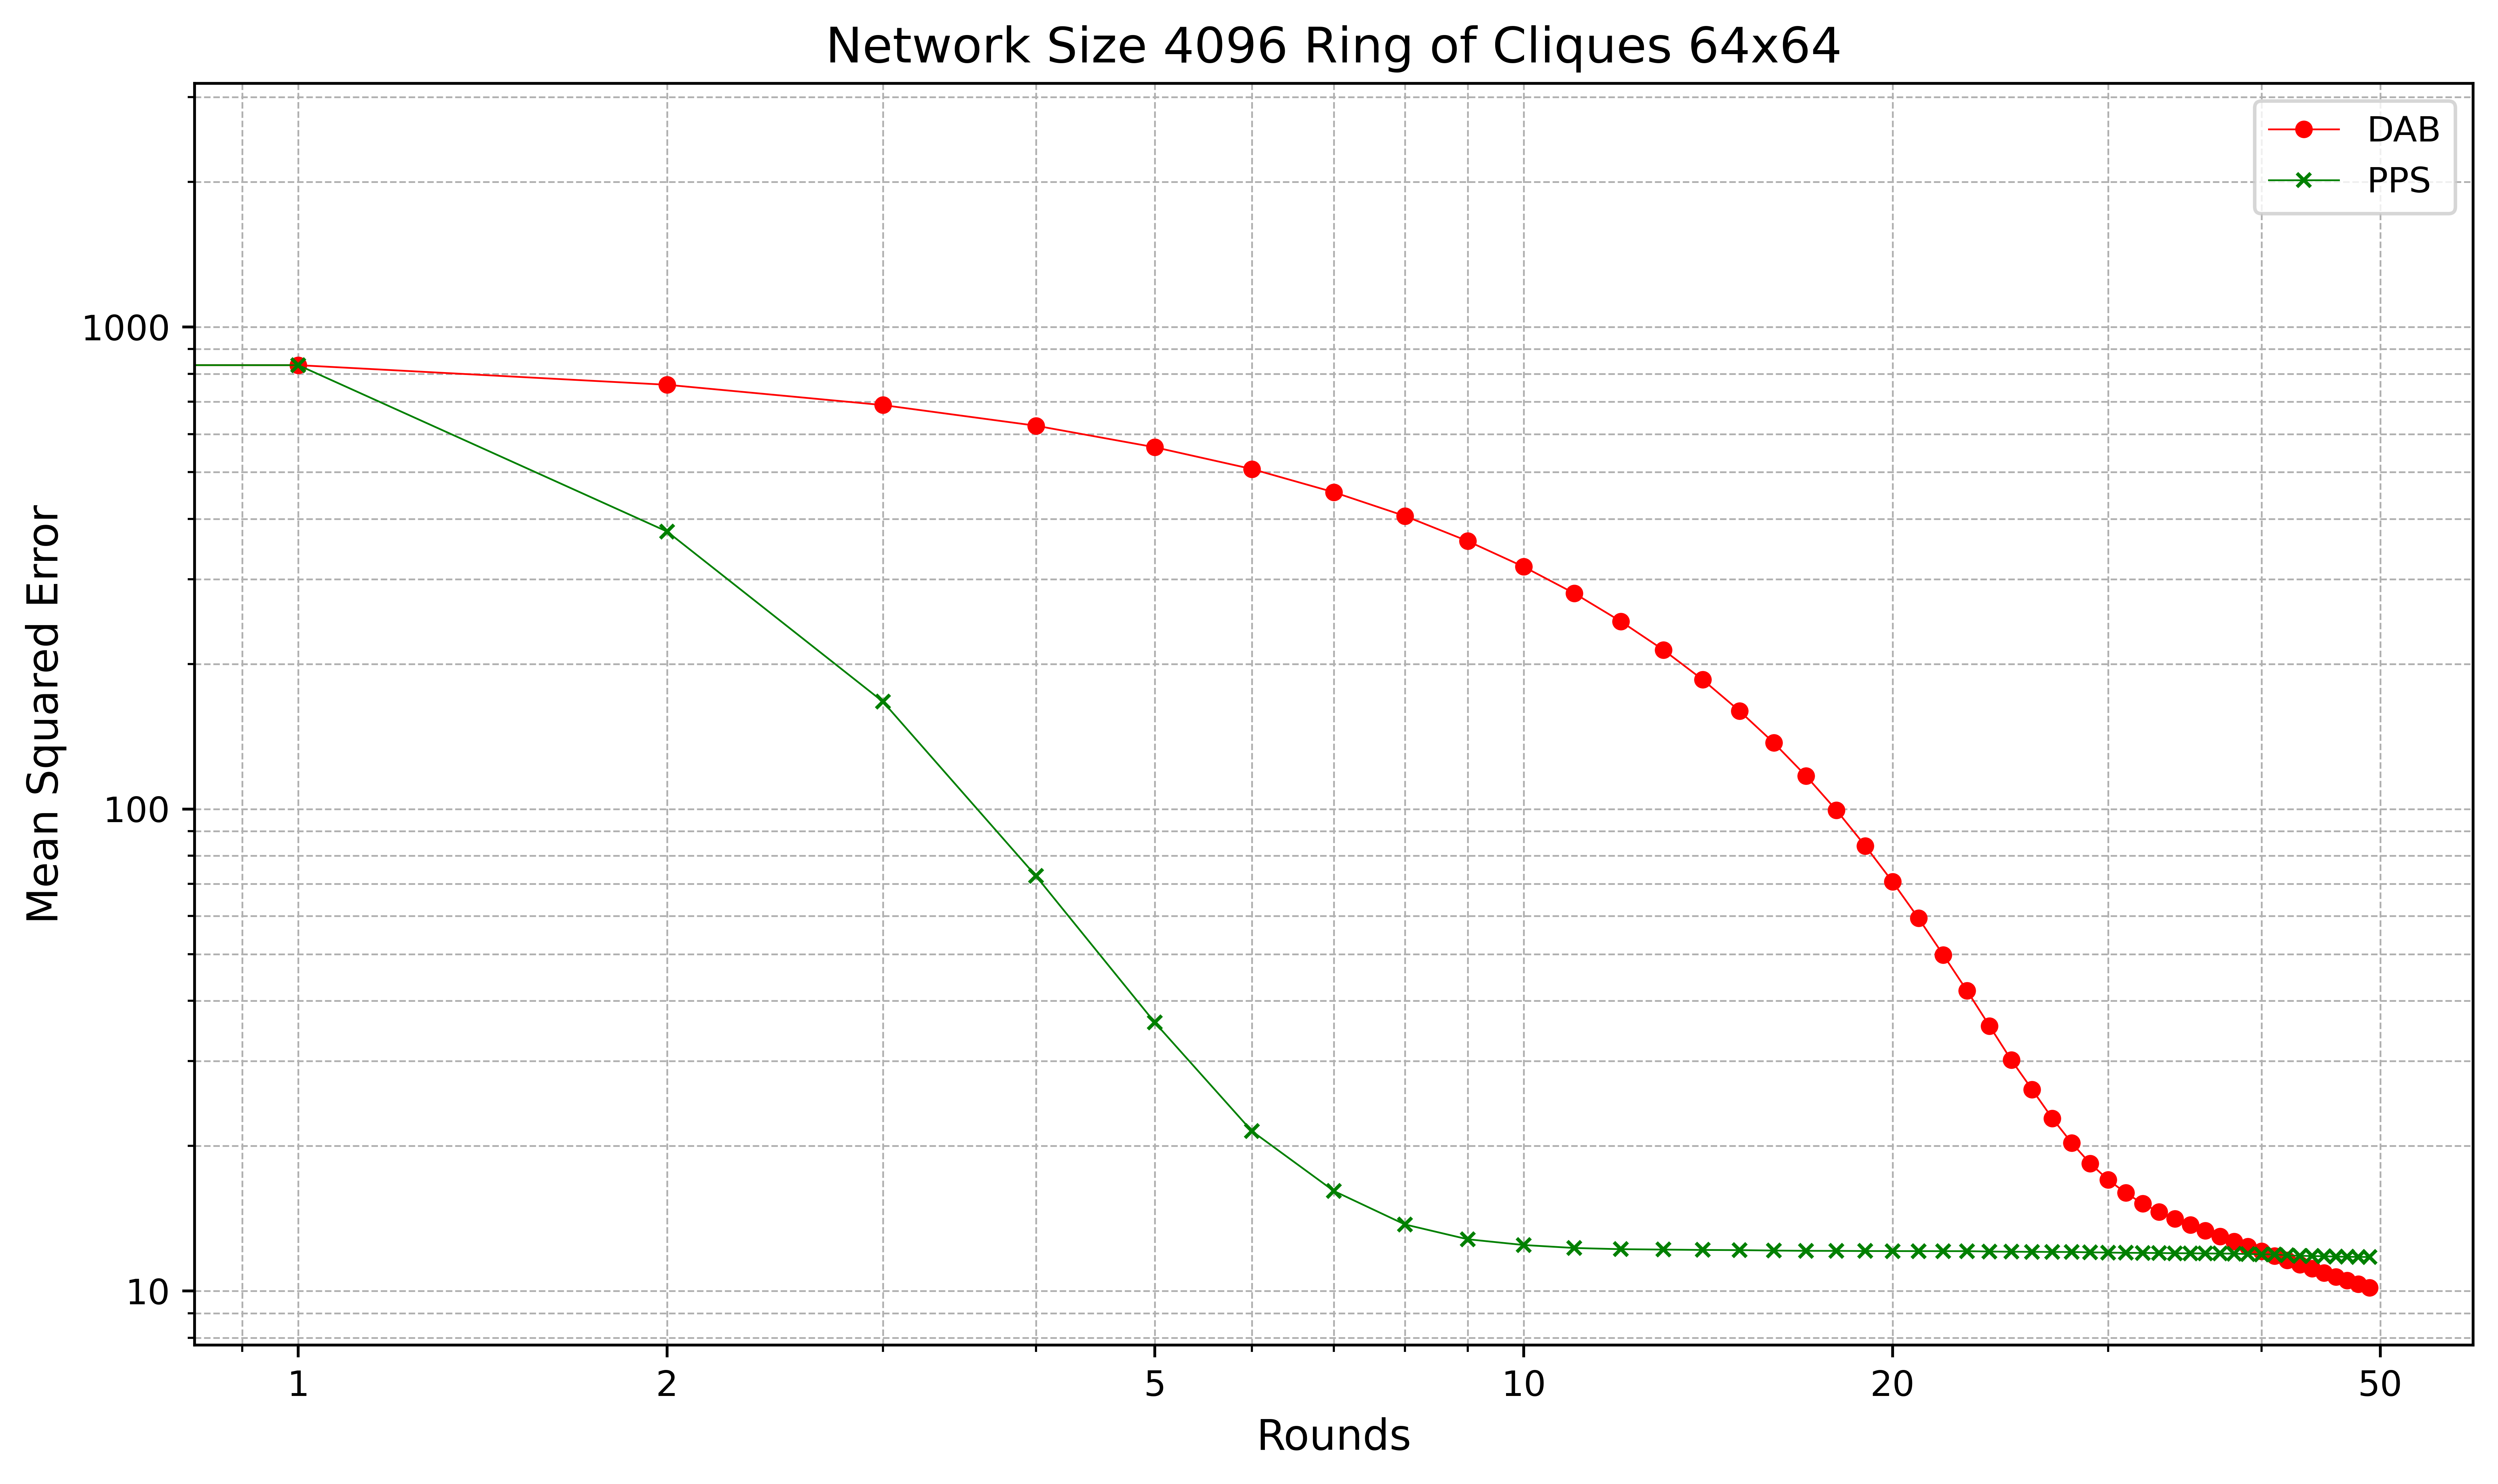
\includegraphics[scale=0.5]{figures/ringOfCliquesSimulations/DAB_vs_PPS_RoC_r50_n4096.png}
    \caption{Ring of cliques: network size $2^{12}$ $(64\times64)$}
    \label{fig:4096ringOfCliques}
\end{figure}

\subsection{Network size: 2\textsuperscript{14}}
\textbf{Figures}: \ref{fig:128x128ringOfCliques}, \ref{fig:32x512ringOfCliques}, \ref{fig:512x32ringOfCliques}\\
\textbf{Observations}: For a ring of cliques with 128 cliques, each with 128 nodes as depicted in \hyperref[fig:128x128ringOfCliques]{Figure} \ref{fig:128x128ringOfCliques}, the PPS is faster at reducing errors than the DAB protocol. As described for the smaller network sizes, the clique size makes a big difference. The larger clique size significantly benefits the PPS protocol, allowing it to reduce the MSE faster than DAB. This becomes very explicit in networks with large clique sizes, such as the $32 \times 512$32 cliques, each with 512 nodes) as shown in \hyperref[fig:32x512ringOfCliques]{Figure} \ref{fig:32x512ringOfCliques}. For the $128 \times 128$ ring of cliques, DAB managed to reduce the MSE of the network to $22.99$ by the 50th round; with a clique size of 512, the MSE of the network in the 50th round is at $443.68$. Meanwhile, the error of the network with PPS decreased from $6.49$ to $2.27$.

For the $512 \times 32$ (512 cliques, each with 32 nodes) ring of cliques, DAB regains its efficiency, outperforming PPS in terms of error reduction. In the 20th round, the MSE of the DAB balanced network falls below that of the PPS balanced network.

Two observations are interesting here:
\begin{enumerate}
    \item The MSE of the PPS balanced network is higher in the $512 \times 32$ simulation compared to the other simulations with the same overall network size $2^{14}$. The MSE of the PPS balanced network by the round 50 is $21.79$
    \item The MSE of the DAB balanced network is lower in the $512 \times 32$ simulation compared to the other simulations with the same overall network size $2^{14}$. The MSE of the DAB balanced network by the round 50 is $11.67$.
\end{enumerate}
This highlights the impact of network structure on the efficiency of load balancing protocols.



\begin{figure}[H]
    \centering
    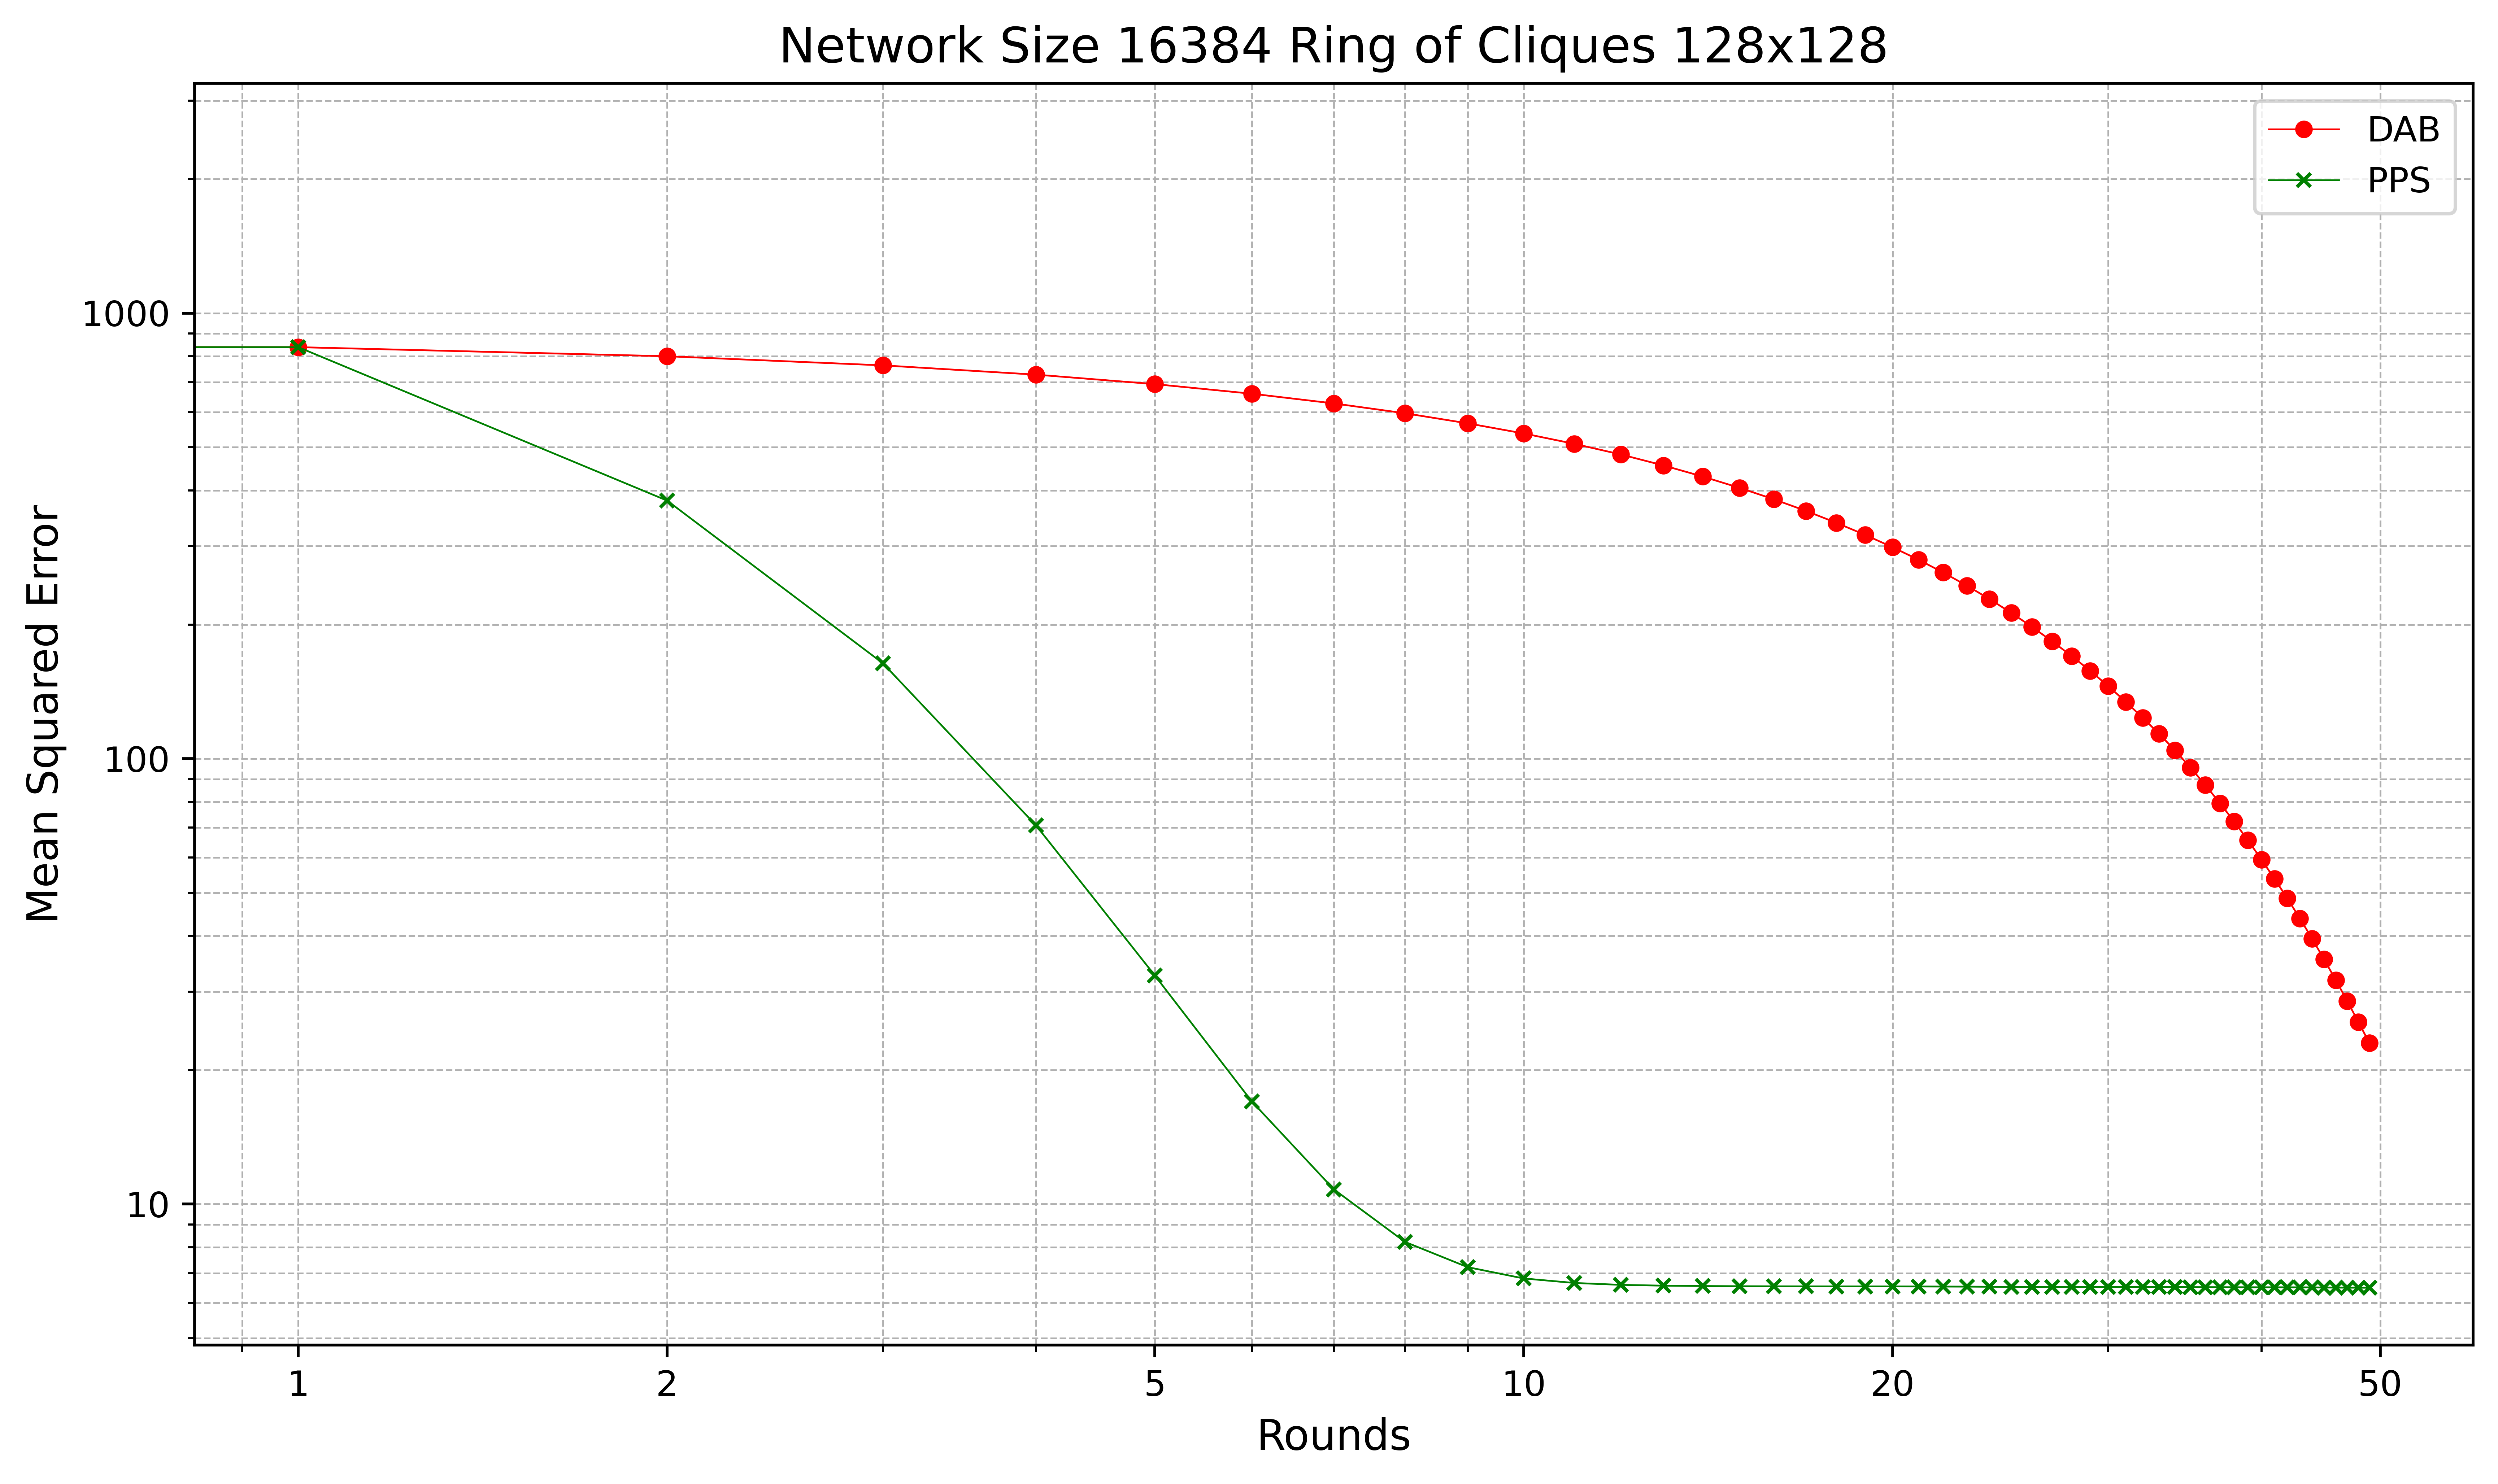
\includegraphics[scale=0.5]{figures/ringOfCliquesSimulations/128x128/DAB_vs_PPS_RoC_r50_n16384.png}
    \caption{Ring of cliques: network size $2^{14}$ $(128\times128)$}
    \label{fig:128x128ringOfCliques}
\end{figure}

\begin{figure}[H]
    \centering
    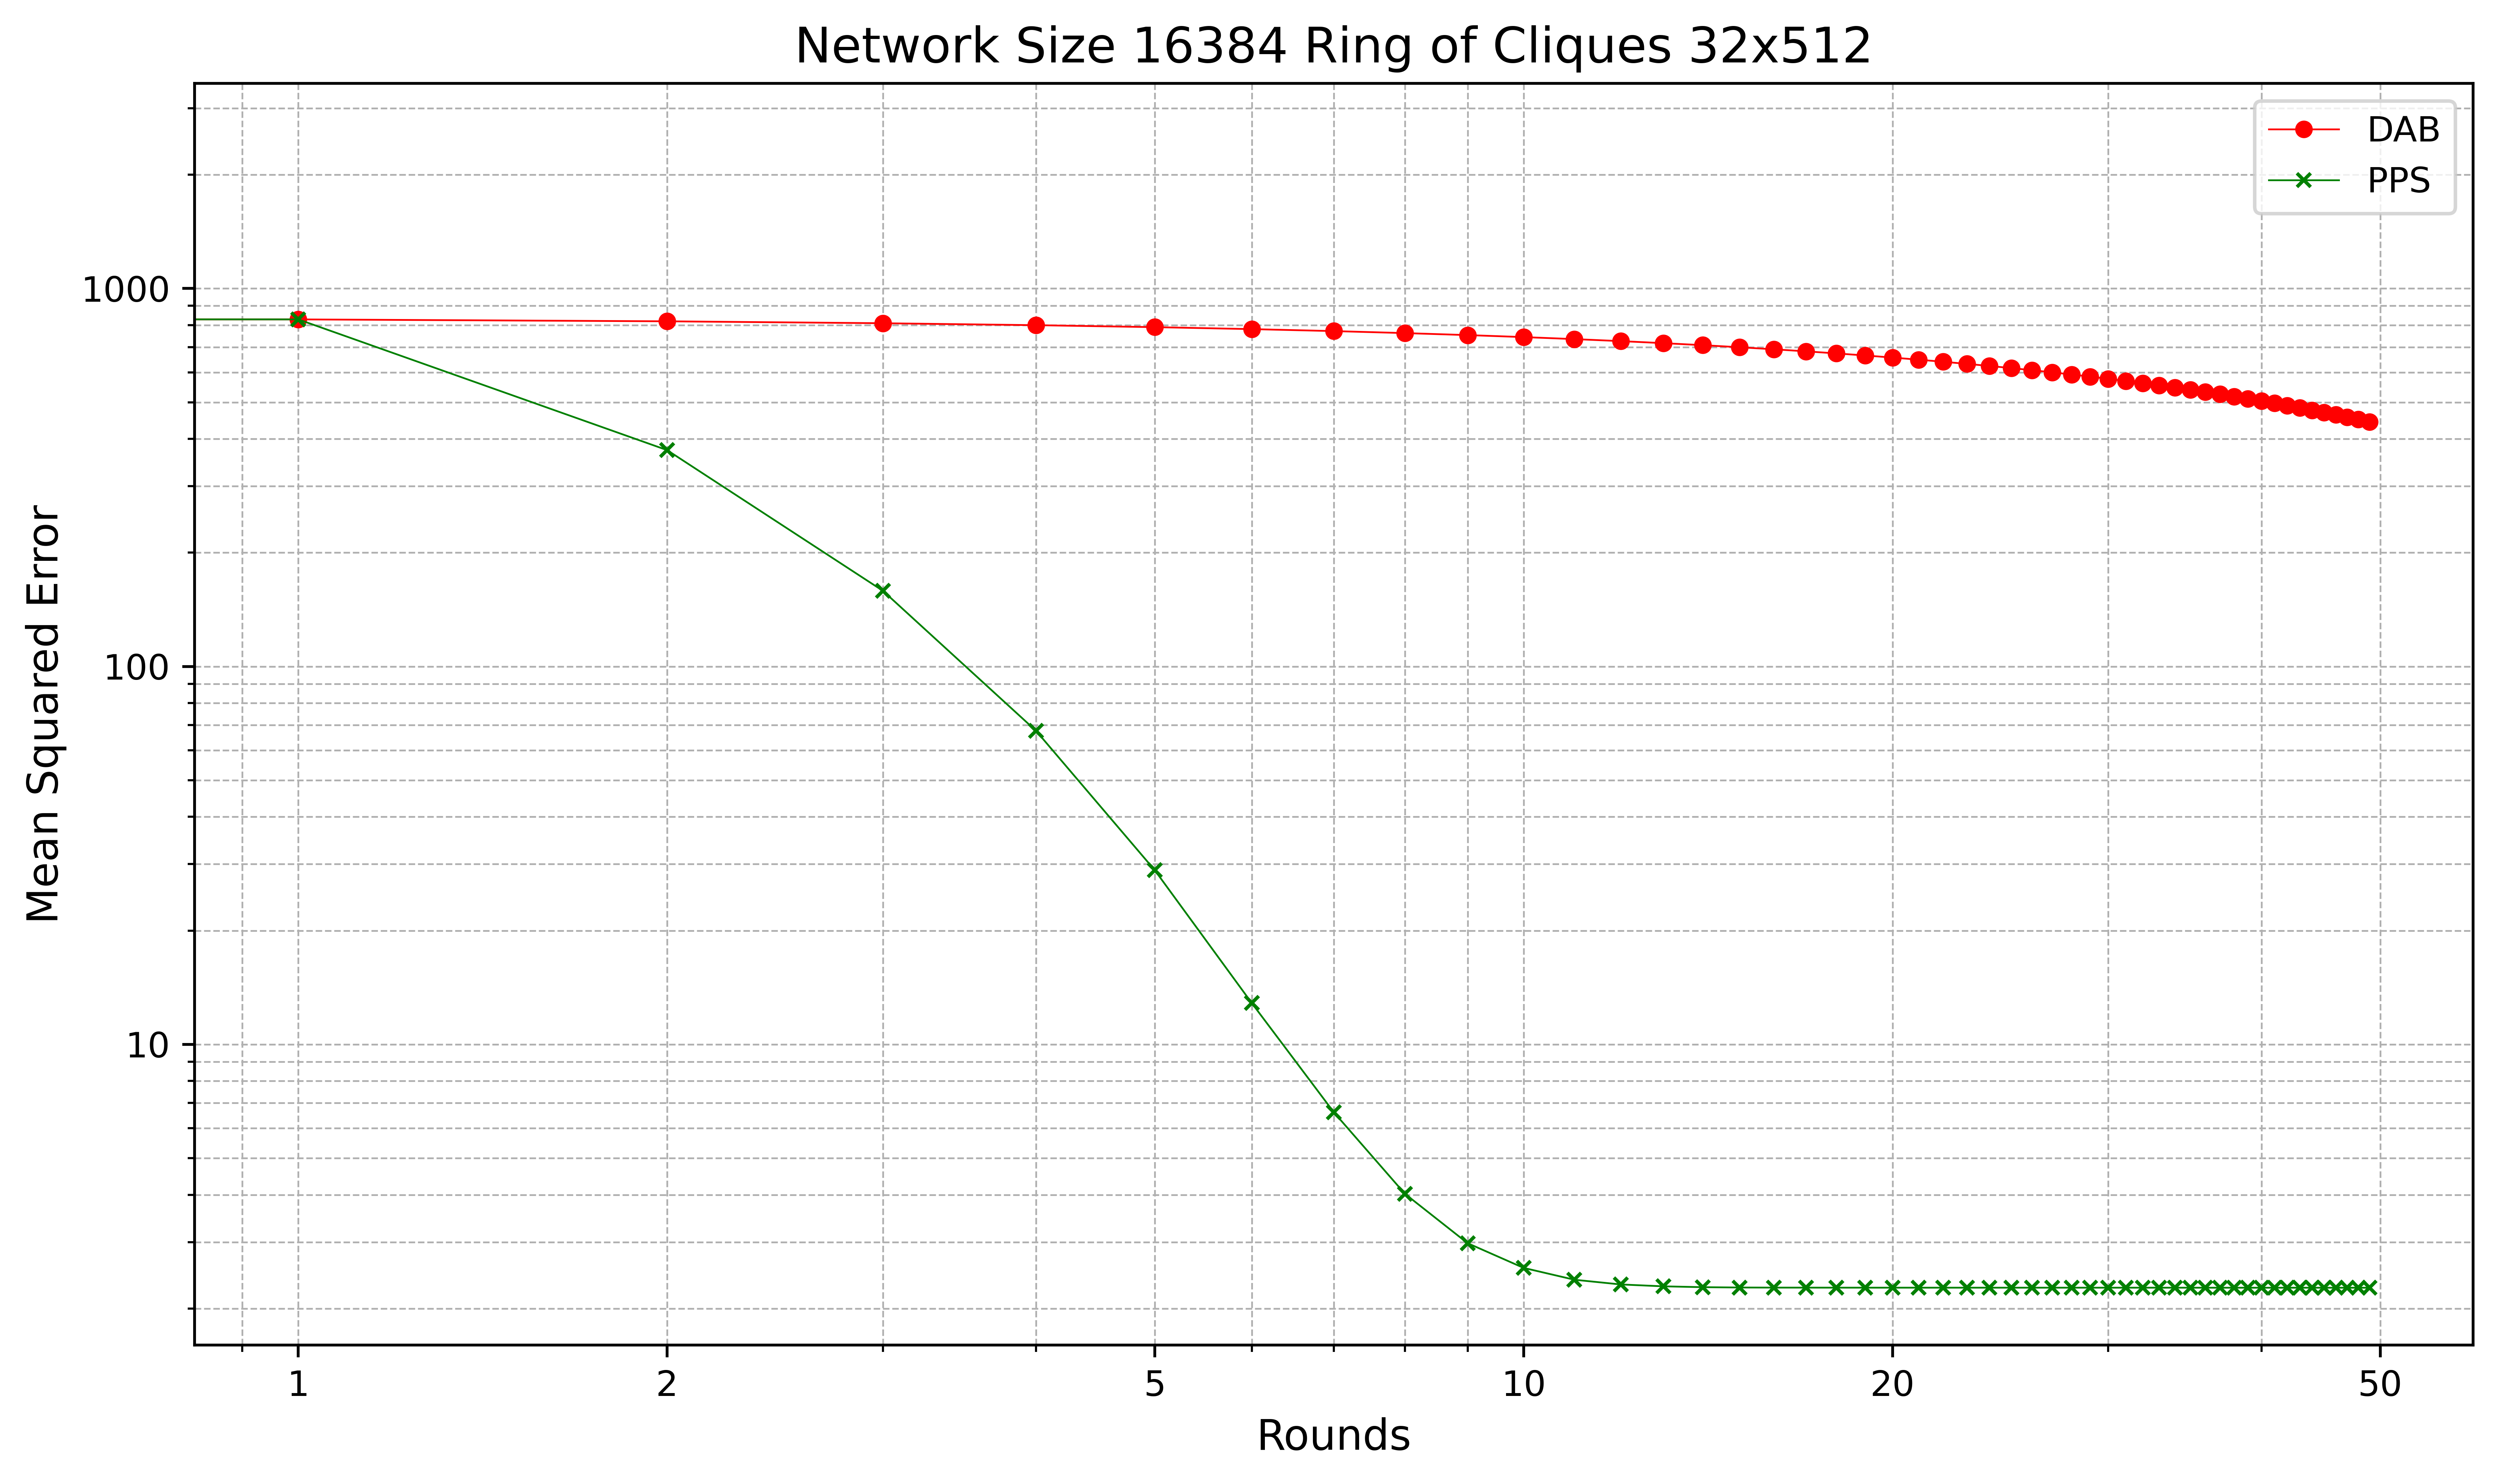
\includegraphics[scale=0.5]{figures/ringOfCliquesSimulations/32x512/DAB_vs_PPS_RoC_r50_n16384.png}
    \caption{Ring of cliques: network size $2^{14}$ $(32\times512)$}
    \label{fig:32x512ringOfCliques}
\end{figure}

\begin{figure}[H]
    \centering
    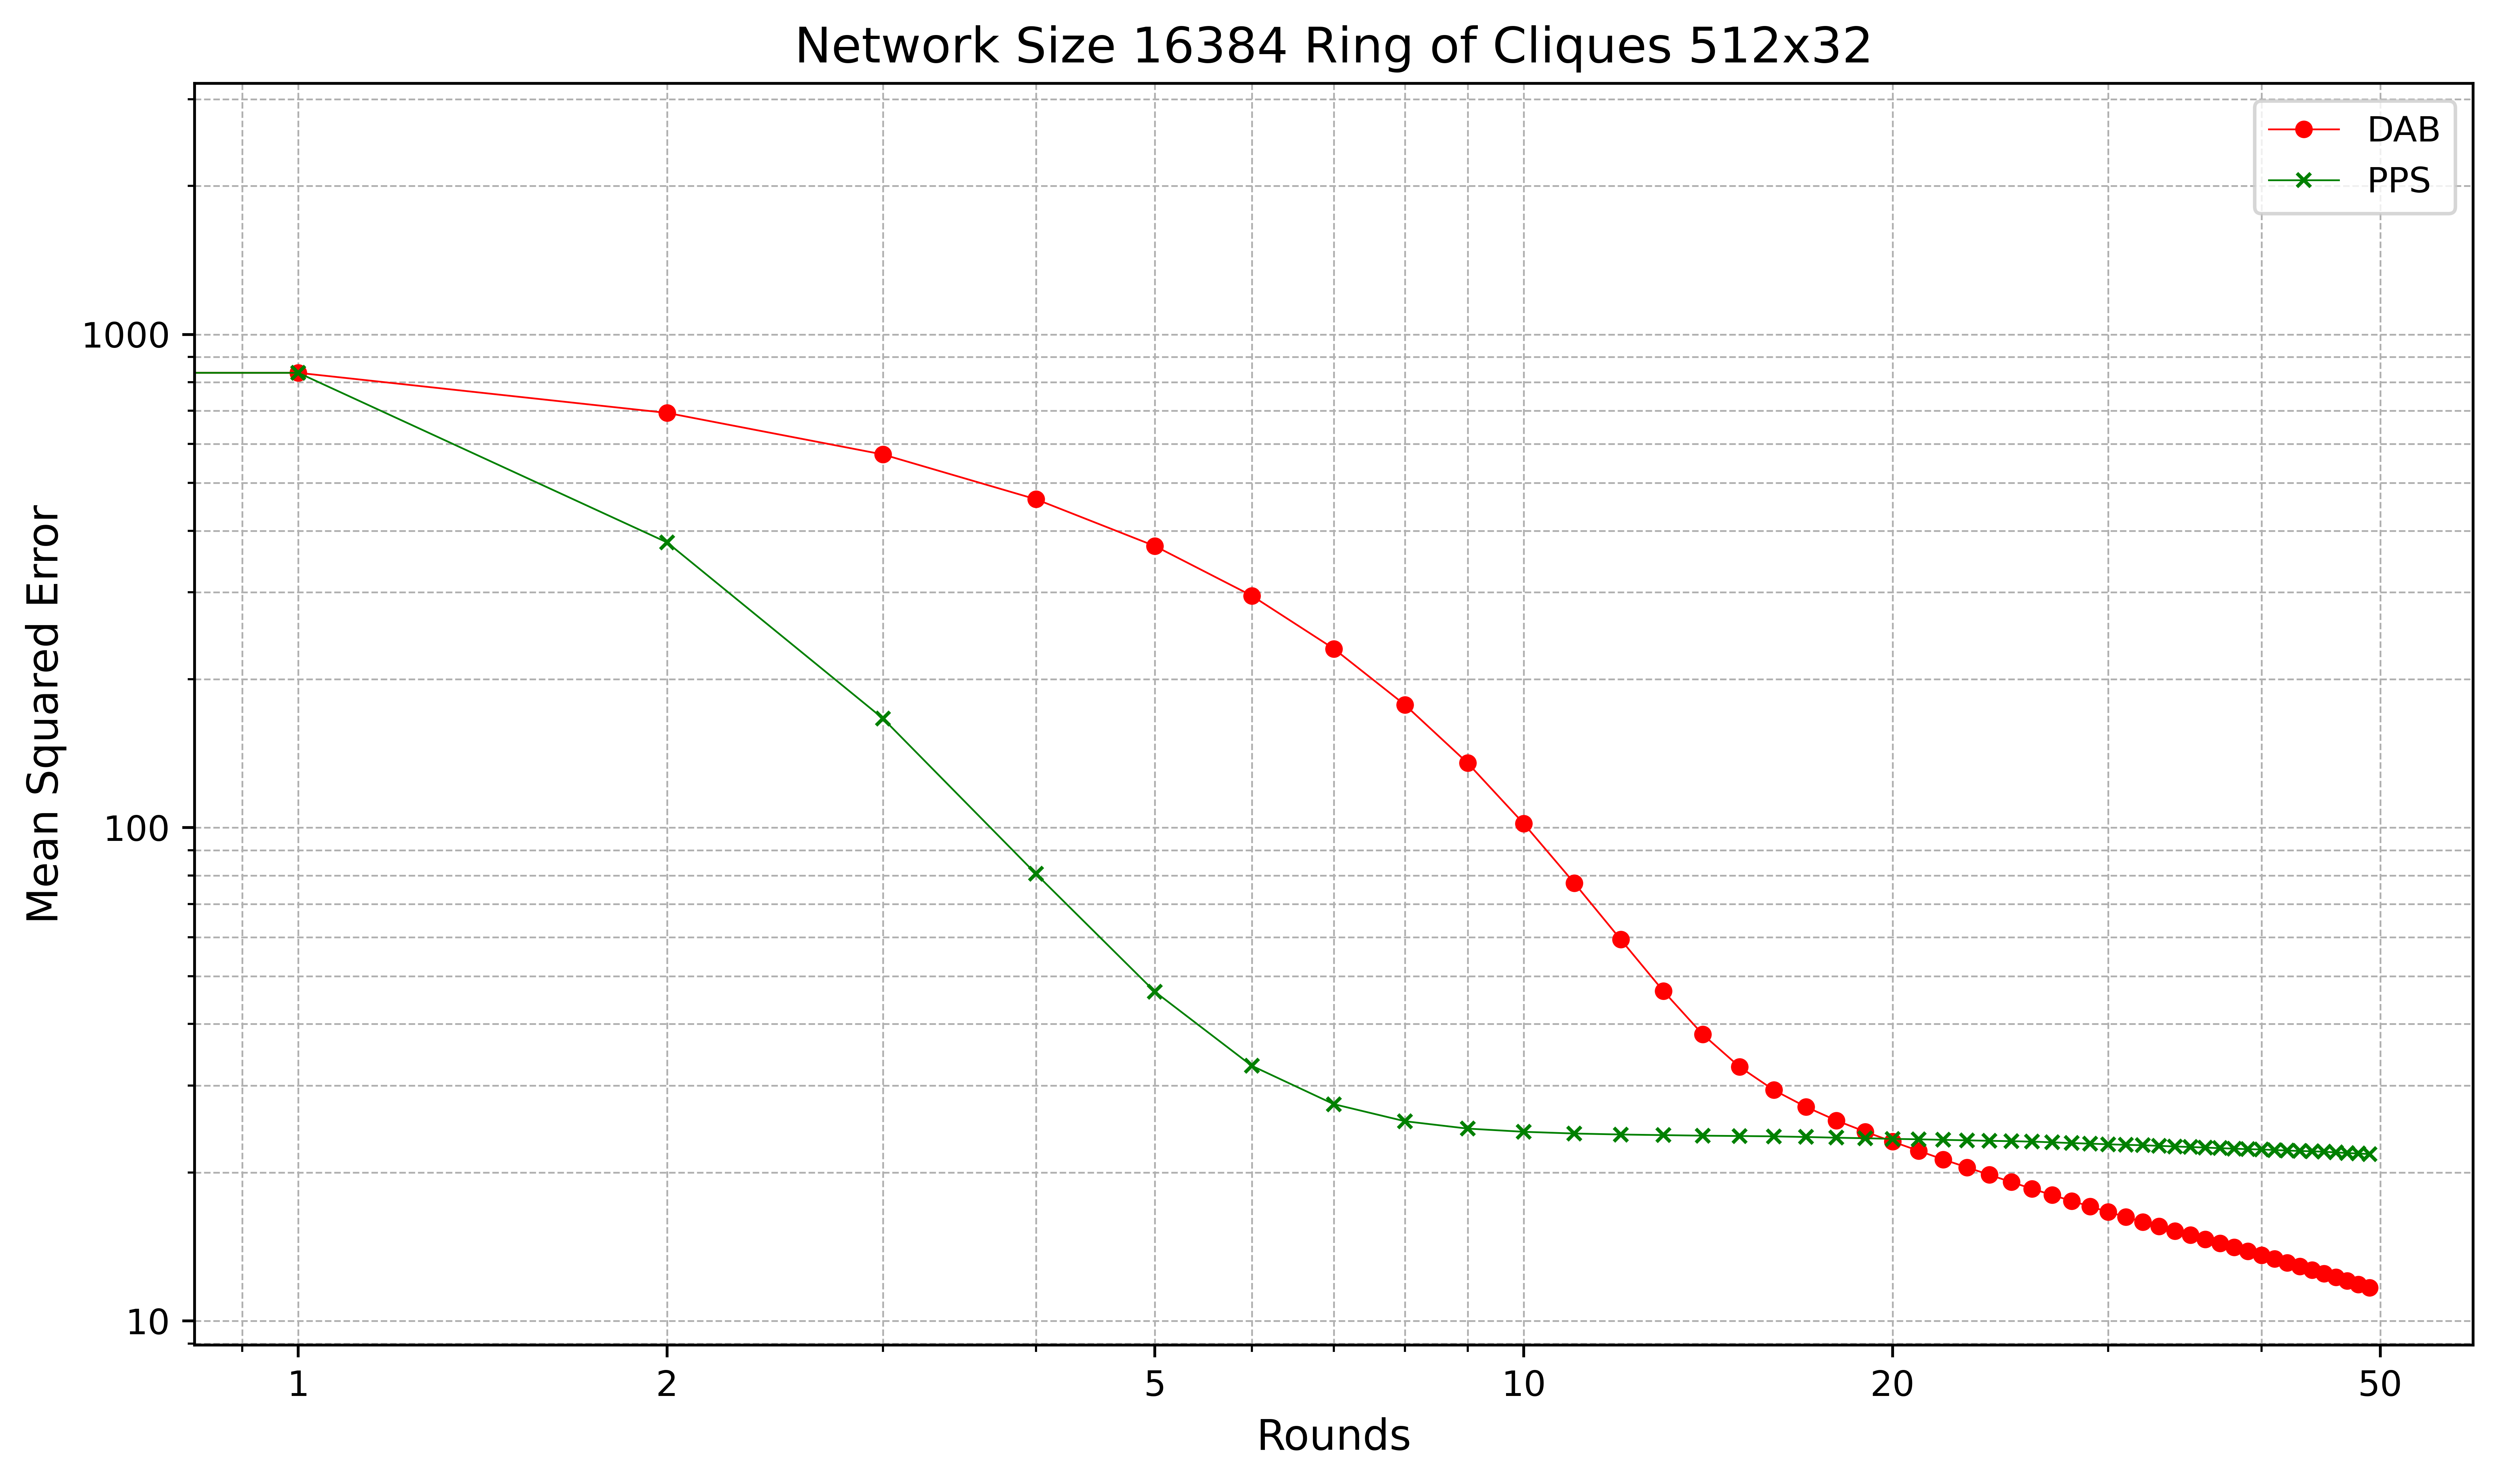
\includegraphics[scale=0.5]{figures/ringOfCliquesSimulations/512x32/DAB_vs_PPS_RoC_r50_n16384.png}
    \caption{Ring of cliques: network size $2^{14}$ $(512\times32)$}
    \label{fig:512x32ringOfCliques}
\end{figure}

\section{Lollipop Graph}
\textbf{The lollipop graph}: A lollipop graph as described in the paper \cite{JonassonLollipopGraphs2000} is a graph that consists of a complete graph and a path graph which are connected by a single node as depicted in \hyperref[fig:lollipopgraphDemo]{figure} \ref{fig:lollipopgraphDemo}. We define a $(m, n)$-Lollipop graph composed of a complete graph with $m$ nodes and a path size of $n$ nodes. A lollipop graph has $m+n$ nodes and $\binom{m}{n}+n$ edges.
\begin{figure}[H]
    \centering
    \scalebox{1}{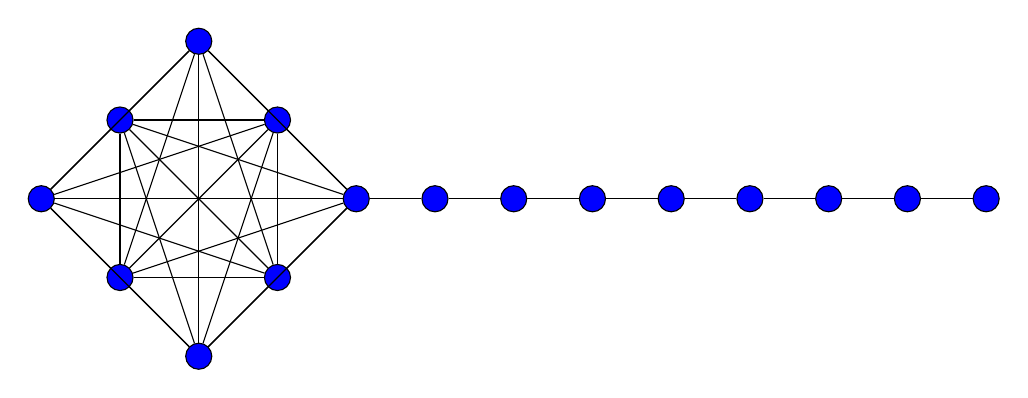
\begin{tikzpicture}
    % Define the 8 vertices in a flat line
    \foreach \i in {1,...,9} {
      \node[draw, fill=blue, circle, minimum size=6pt] (v\i) at (\i, 0) {};
    }
    
    % Draw edges to connect each vertex to the next
    \foreach \i in {1,...,8} {
      \pgfmathtruncatemacro{\j}{\i+1}
      \draw (v\i) -- (v\j);
    }

    % Define additional vertices for the complete graph on v1, centered around v1
    \node[draw, fill=blue, circle, minimum size=6pt] (c1) at (0,1) {};
    \node[draw, fill=blue, circle, minimum size=6pt] (c2) at (0,-1) {};
    \node[draw, fill=blue, circle, minimum size=6pt] (c3) at (-1,2) {};
    \node[draw, fill=blue, circle, minimum size=6pt] (c4) at (-1,-2) {};
    \node[draw, fill=blue, circle, minimum size=6pt] (c5) at (-2,-1) {};
    \node[draw, fill=blue, circle, minimum size=6pt] (c6) at (-2,1) {};
    \node[draw, fill=blue, circle, minimum size=6pt] (c7) at (-3, 0) {};
    
    % Connect the complete graph nodes to v1
    \foreach \k in {1,2,3,4,5,6,7} {
      \draw (v1) -- (c\k);
    }

    % Draw edges between the new nodes to form a complete graph
    \foreach \a in {1,2,3,4,5,6,7} {
      \foreach \b in {\a,...,7} {
        \ifnum\a=\b\else
        \draw (c\a) -- (c\b);
        \fi
      }
    }

  \end{tikzpicture}}
    \caption{Lollipop graph: network size 16}
    \label{fig:lollipopgraphDemo}
\end{figure}

\subsection{Network sizes: 2\textsuperscript{4}, 2\textsuperscript{8} and 2\textsuperscript{12}}
\textbf{Figures}: \ref{fig:8+8lollipop}, \ref{fig:128+128lollipop}, \ref{fig:2048+2048lollipop}\\
\textbf{Observations}: For the $(8, 8)$-lollipop graph DAB shows a slight advantage over PPS. In the $(128, 128)$-lollipop graph this changes. Although DAB recovers after a poor start, the difference in MSE between the two networks expands significantly by the 10th round. For instance, in the 12th round, the MSE of the DAB balanced network is at $232.13$, while the PPS network is at $38.81$. By the 30th round, the MSE of the DAB balanced network decreases to 68.36, compared to 16.66 for the PPS network. Finally, in the 50th round, the MSE for the DAB managed network is 15.20, and for the PPS managed network, it is 11.69.

This trend of PPS having a advantage becomes more significant with larger clique sizes (i.e., larger numbers of nodes assigned to the cliques). For example, in the $(2048, 2048)$-lollipop graphthe MSE in the 50th round for the two networks varies a lot. While the PPS managed network's MSE is around 20, the DAB managed graph's MSE is around 378, implying the inability of DAB to handle large network sizes with high connectivity as efficiently as PPS. This observation is already made for the complete graph and the ring of cliques with large clique sizes. \\

\begin{figure}[H]
    \centering
    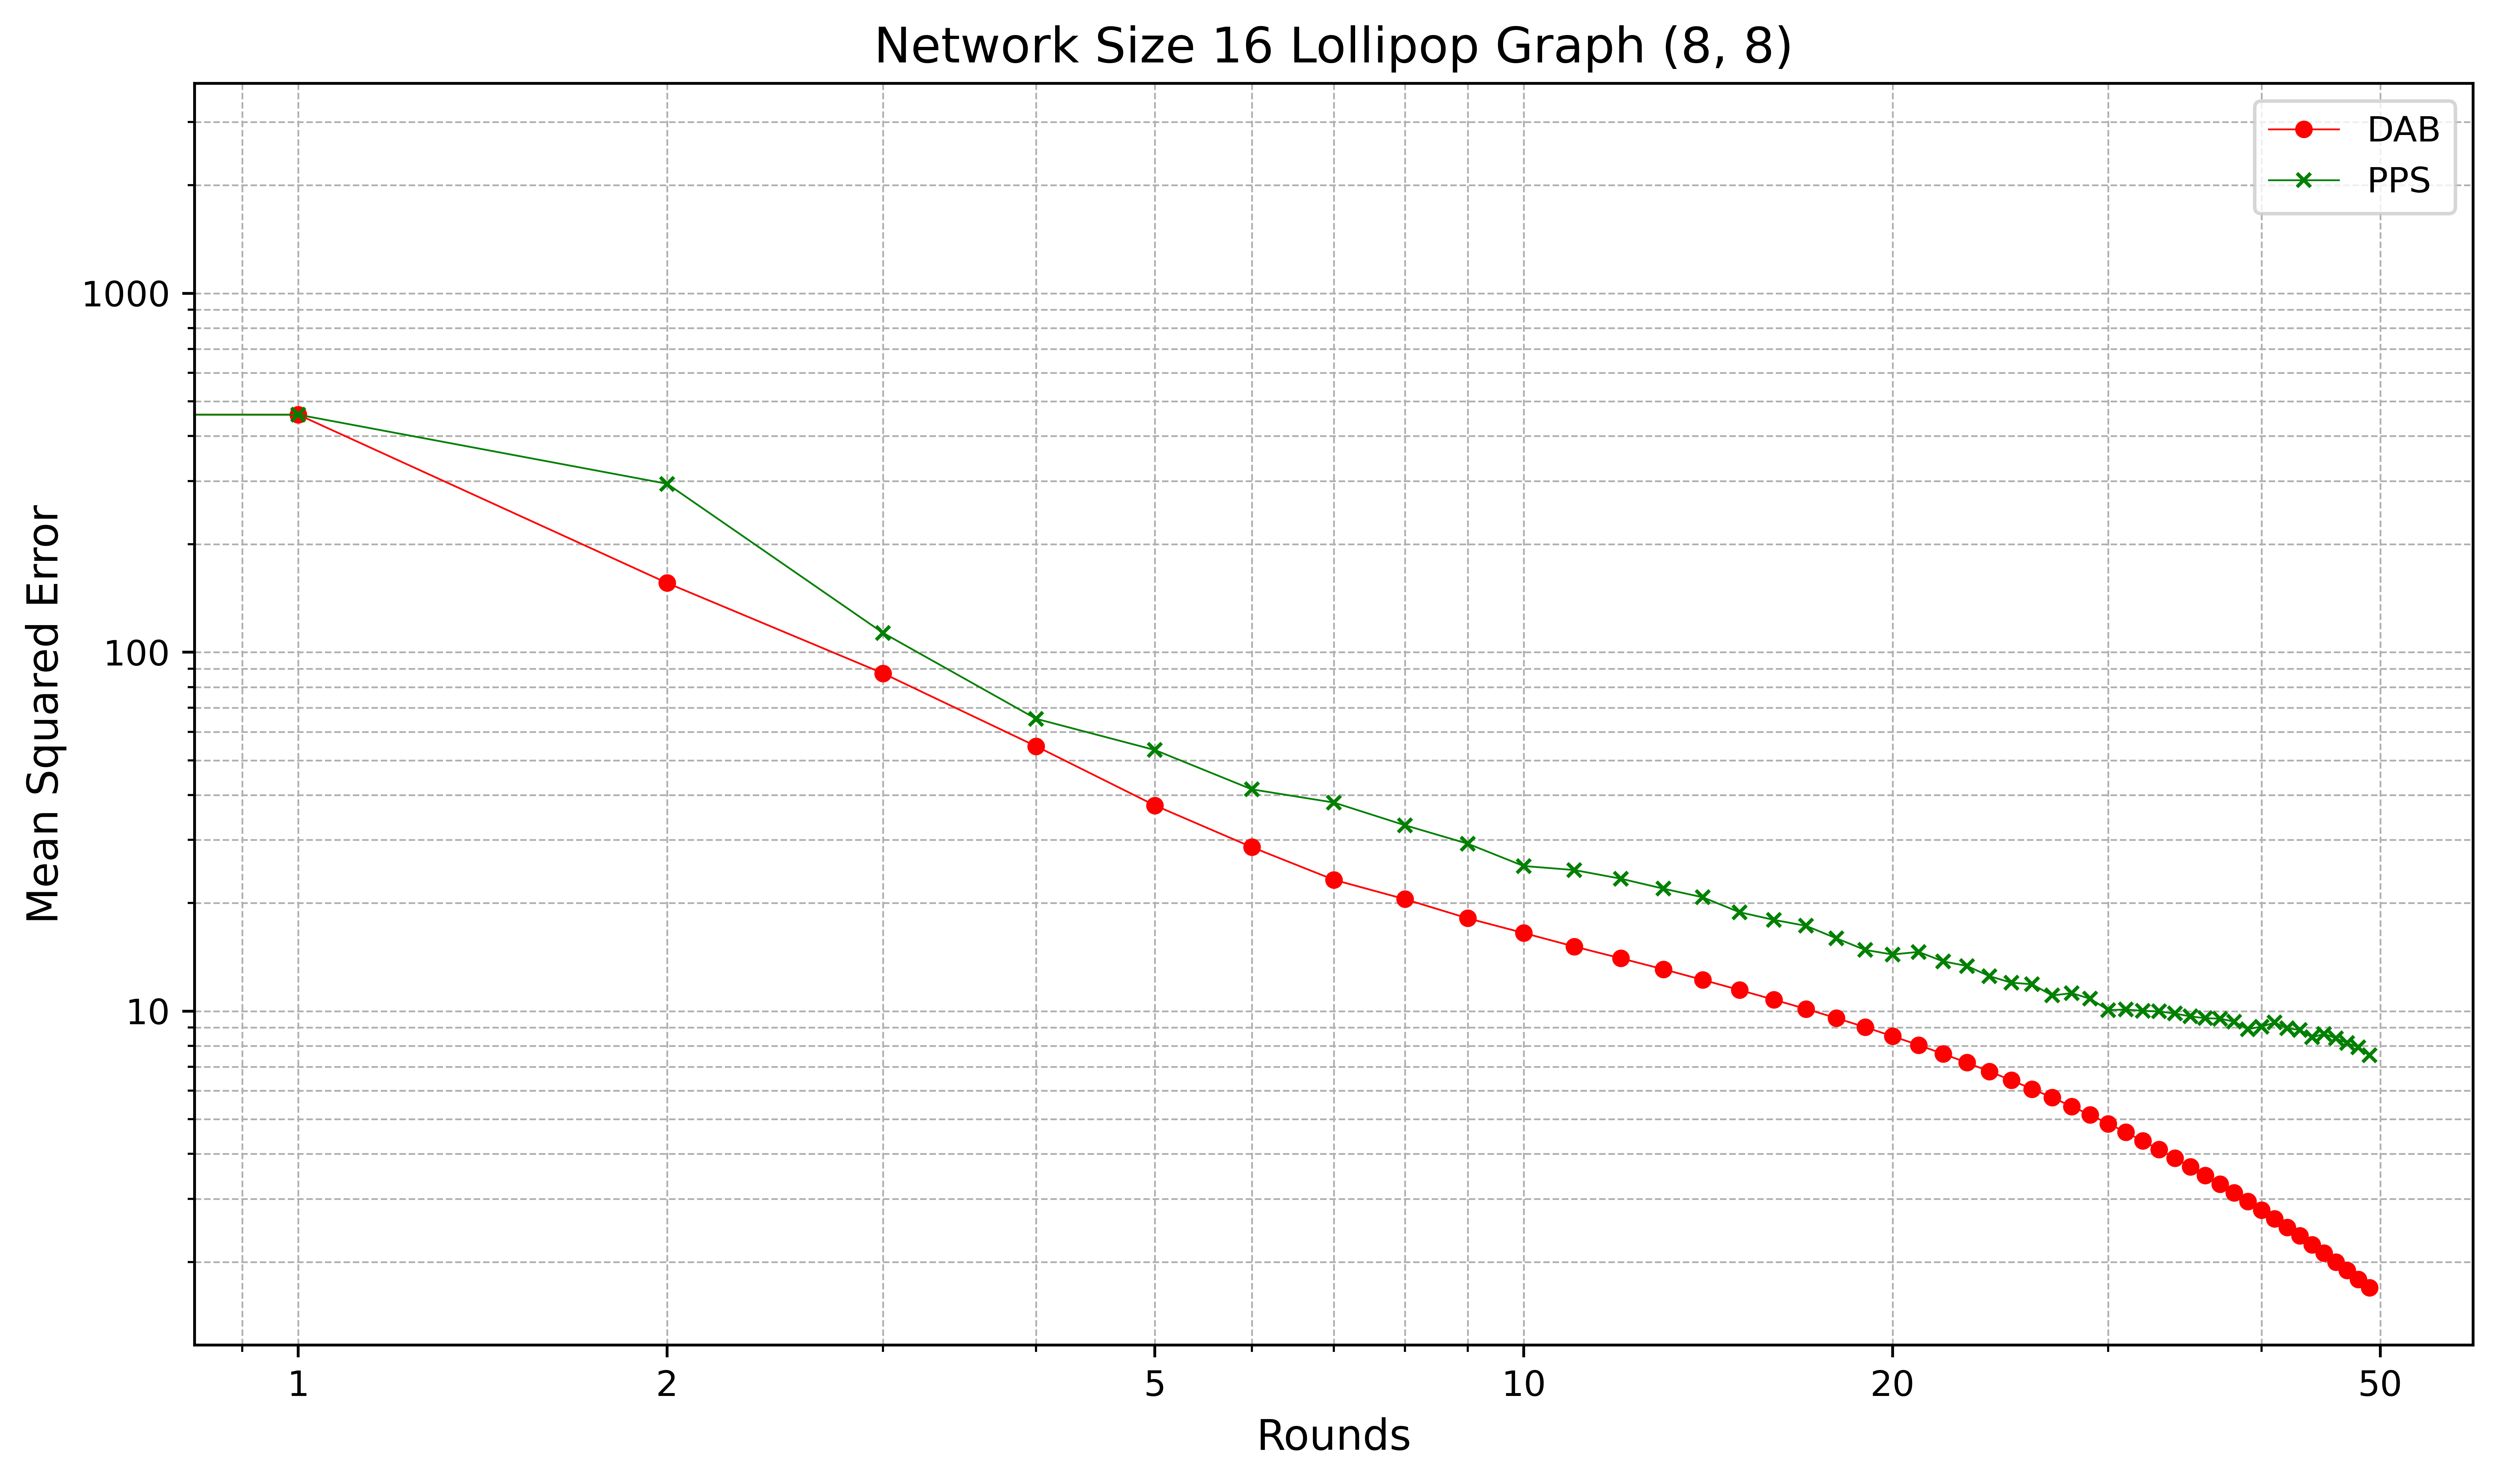
\includegraphics[scale=0.5]{figures/lollipopGraphSimulations/DAB_vs_PPS_LG_r50_n16.png}
    \caption{Lollipop graph: network size $2^{4}$ $(8, 8)$}
    \label{fig:8+8lollipop}
\end{figure}

\begin{figure}[H]
    \centering
    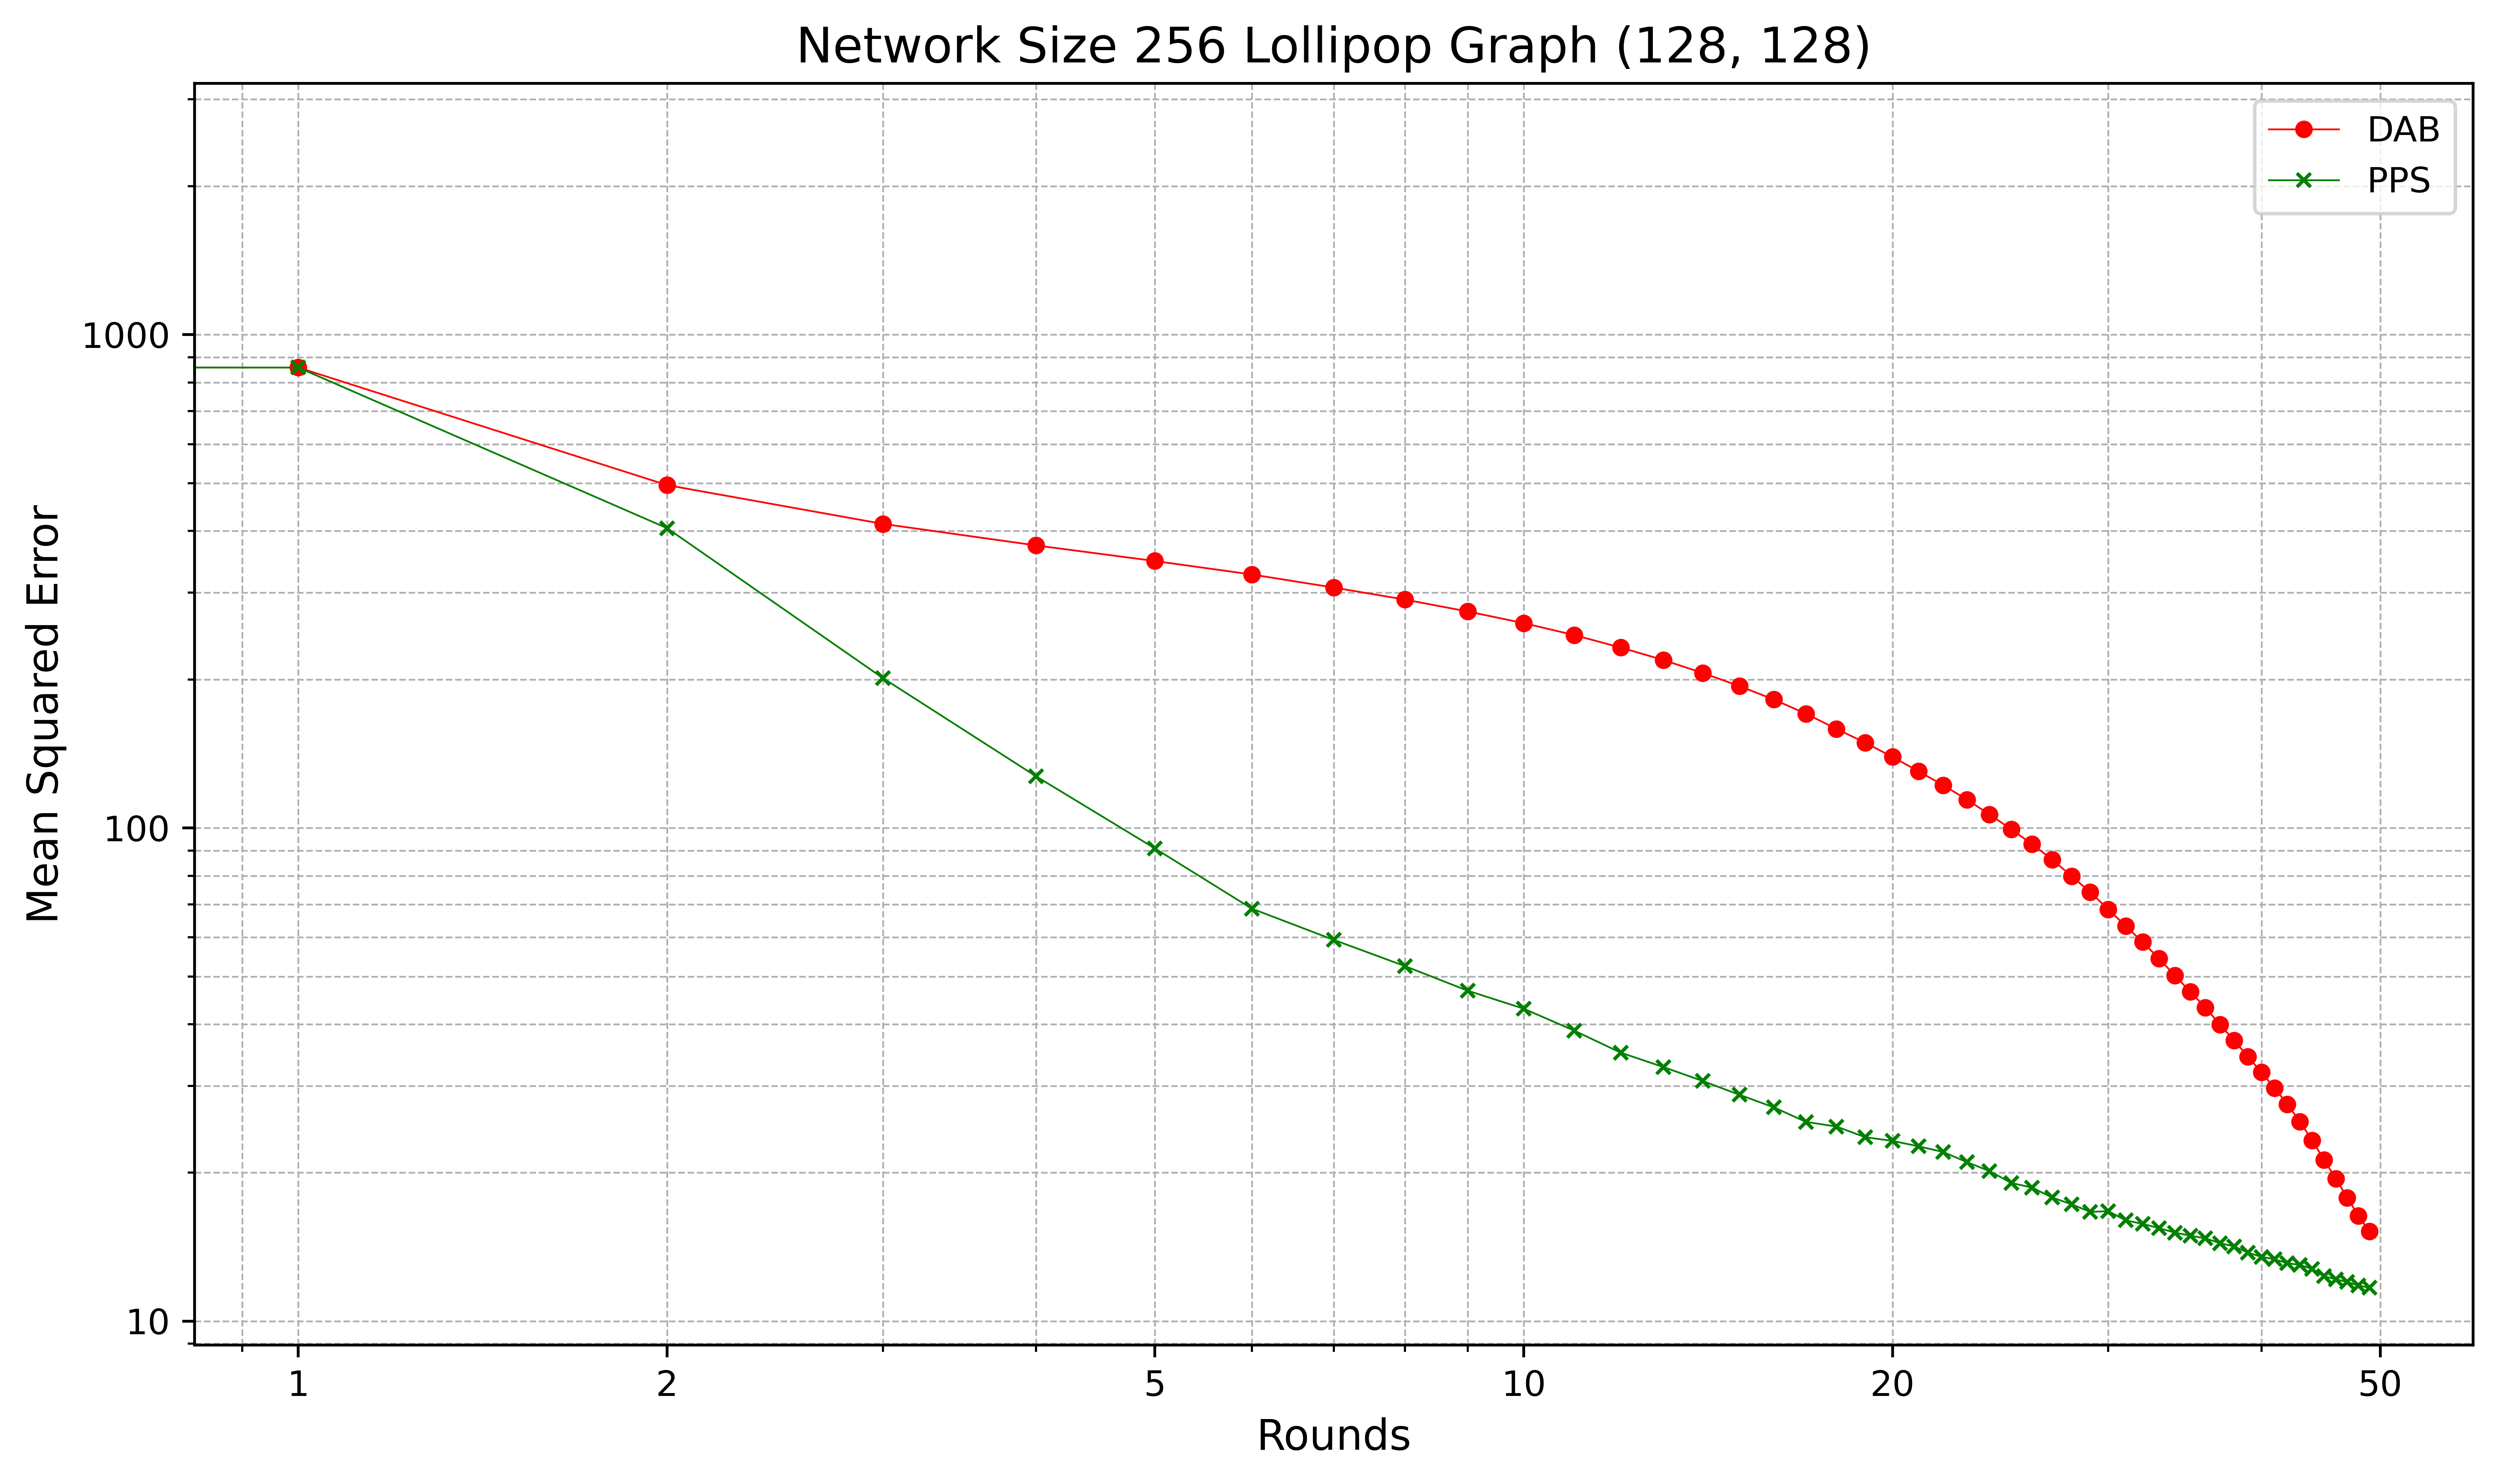
\includegraphics[scale=0.5]{figures/lollipopGraphSimulations/DAB_vs_PPS_LG_r50_n256.png}
    \caption{Lollipop graph: network size $2^{8}$ $(128, 128)$}
    \label{fig:128+128lollipop}
\end{figure}

\begin{figure}[H]
    \centering
    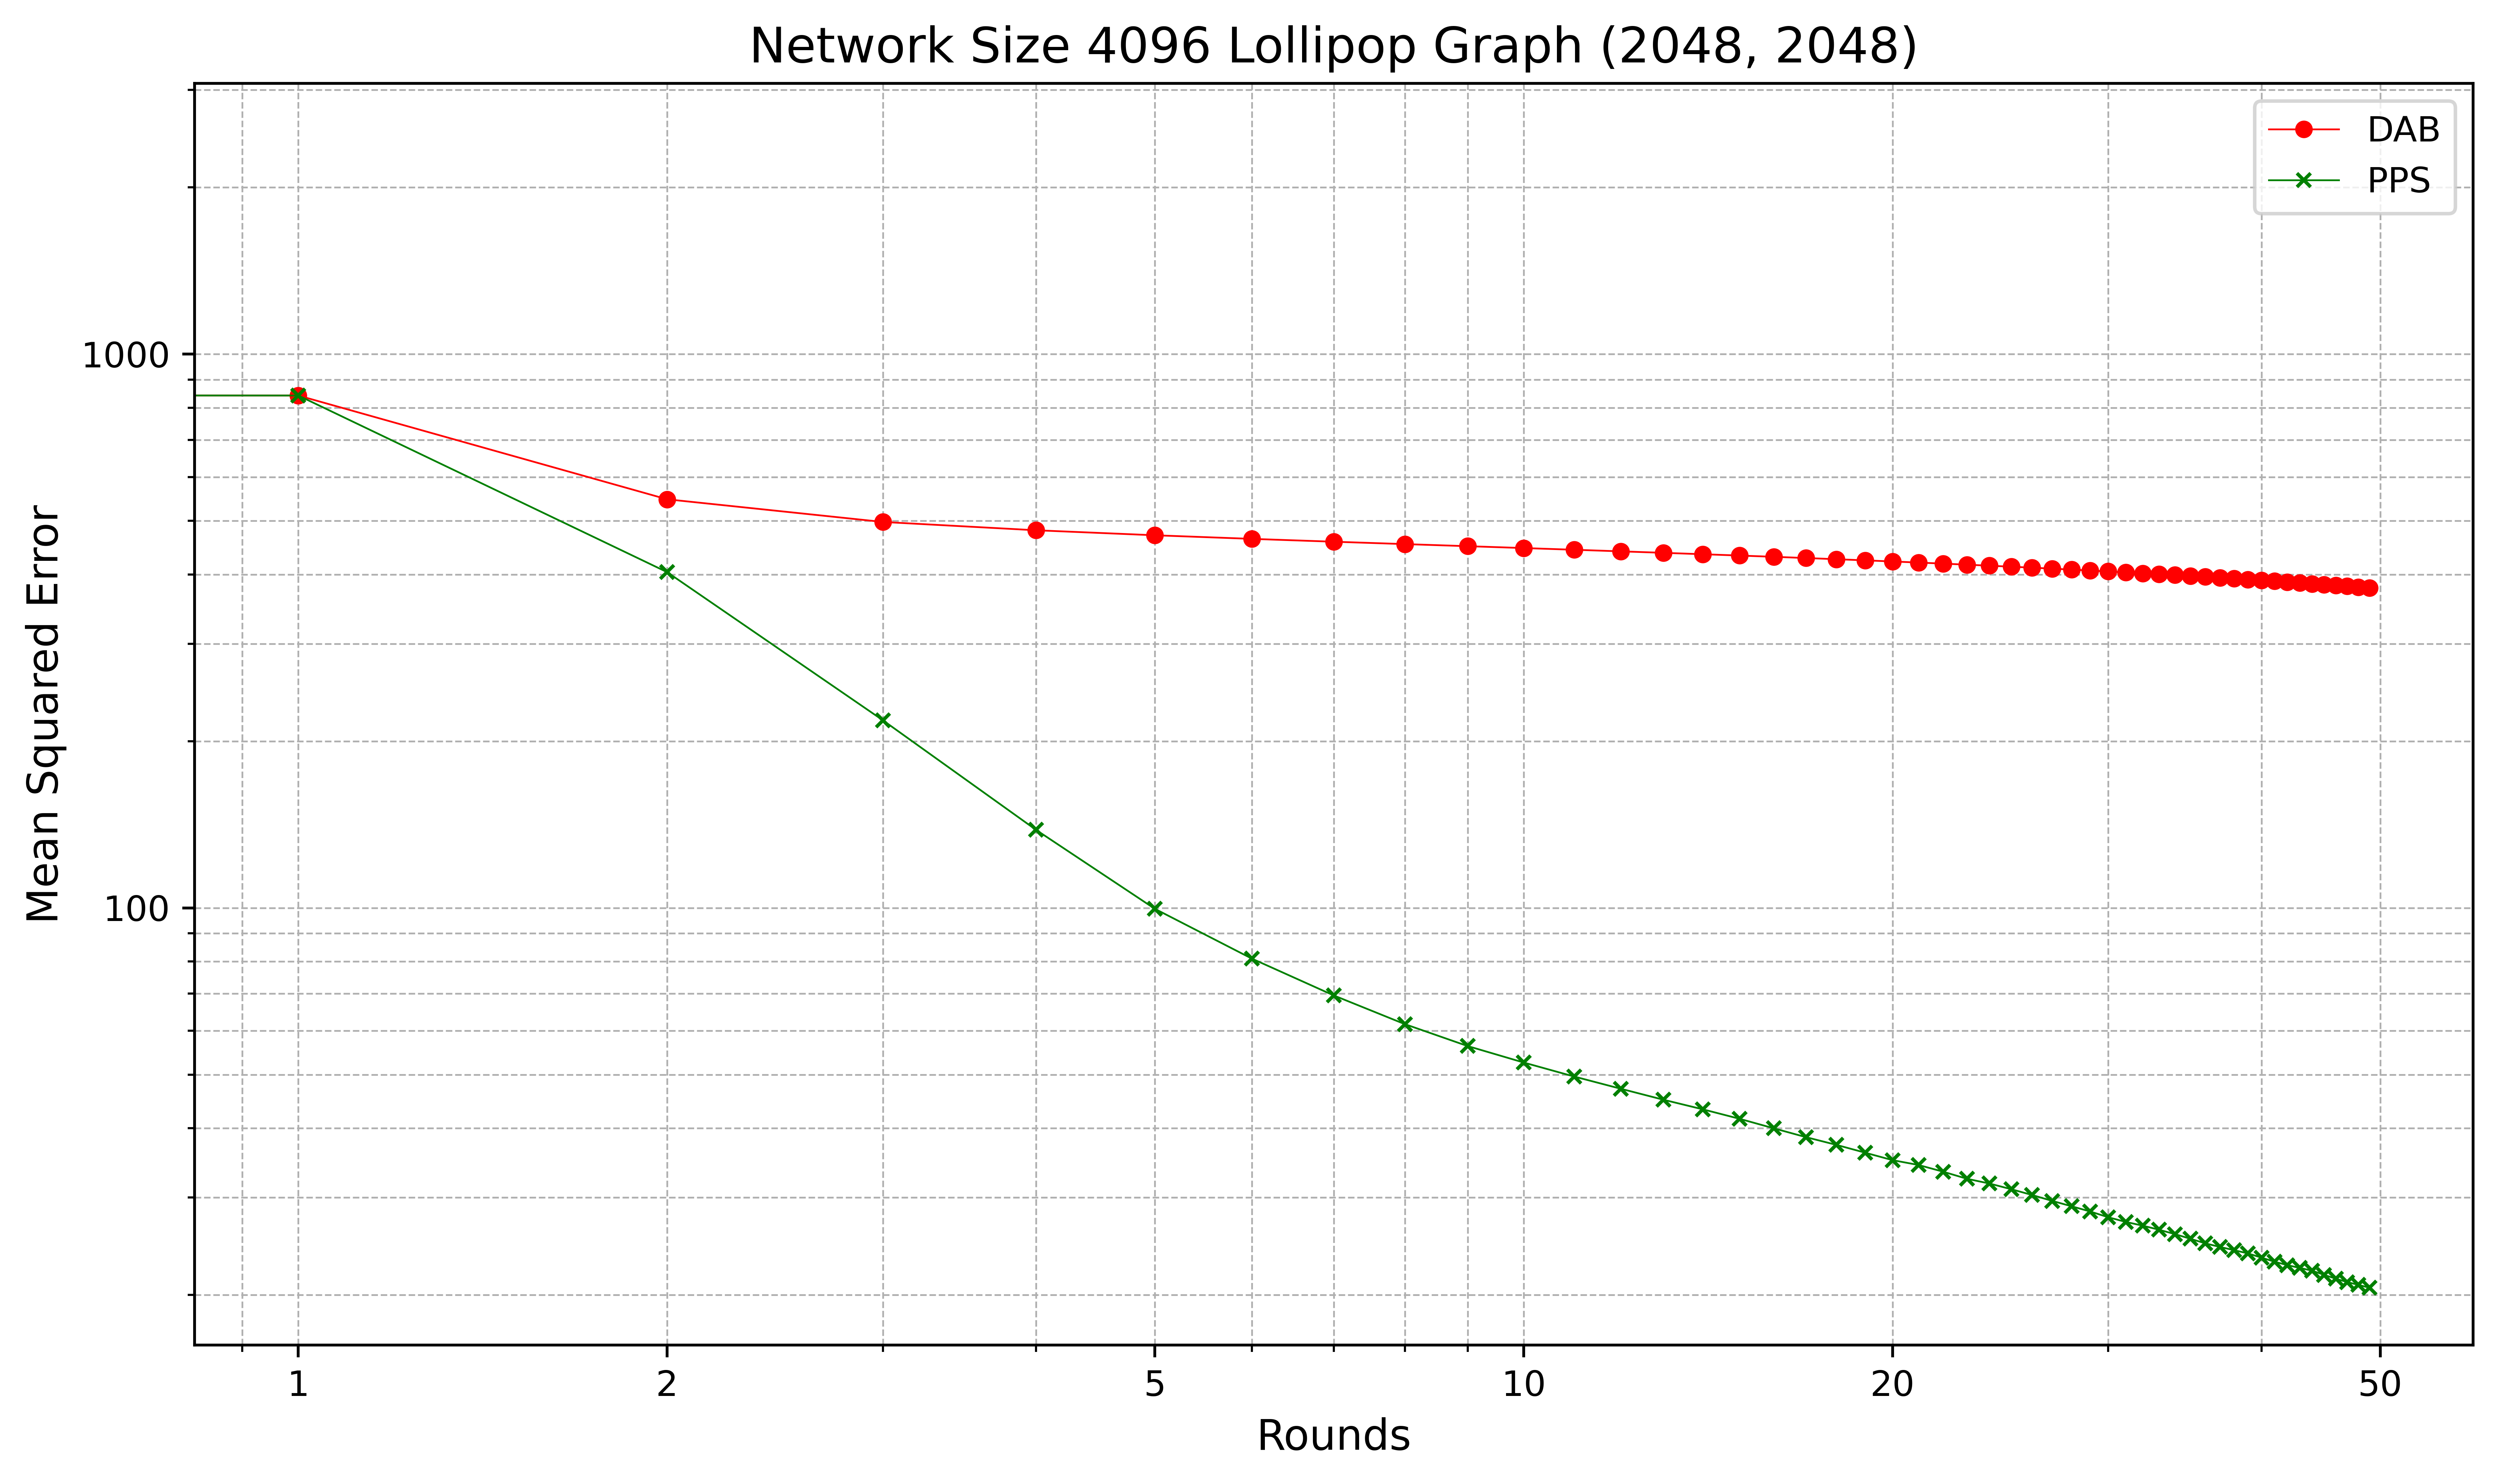
\includegraphics[scale=0.5]{figures/lollipopGraphSimulations/DAB_vs_PPS_LG_r50_n4096.png}
    \caption{Lollipop graph: network size $2^{12}$ $(2048, 2048)$}
    \label{fig:2048+2048lollipop}
\end{figure}

Note: For the Lollipop graph, no simulations were conducted for the network size $2^{14}$ due to the time required to obtain reliable results. That is why we decided to simulate for at most $10^{4}$ (in the \hyperref[chap:appendix]{Appendix}) nodes.
